%loads the class that provides the titlepage and some general packages.
\documentclass{UniVieCS_Thesis} 

%add the additional packages and macros that you want to use
\input{packages_macros}

% important update for glossaries, before document 
\loadglsentries{C) Back Matter/acronyms.tex}
\loadglsentries{C) Back Matter/glossary.tex} 
\makeglossaries %https://www.overleaf.com/learn/latex/glossaries

%shows fixme notes
%\fxsetup{status=draft} % comment/delete this line if you want to your final output

\usepackage[british]{babel} %if changed to \usepackage[ngerman]{babel} "Table of contents" changes to "Inhaltsverzeichnis", "abstract" becomes "Zusammenfassung" and "references" is translated to "Literatur".


%remove all the things you don't need and add all the things you need. you can also change the order of the elements at your will.
\begin{document}
    % set depth of subsubsection 
    \setcounter{secnumdepth}{3}
    
    %Start with front matter
    
    %Choose the titlepage you want to use
    
    \input{A) Front Matter/titlepage} %Creates the titlepage
    %\input{A) Front Matter/titlepage_bsc} %Creates the titlepage
    %\input{A) Front Matter/titlepage_phd} %Creates the titlepage
    
    \clearpage
	\frontmatter{}
	%\input{A) Front Matter/acknowledgements} %adds the aknowledgements
			%Please consider the following section of the "Formvorschriften für die gedruckte Version"
	%Im Anhang ist eine Zusammenfassung (Abstract) mitzubinden. 
	%Ist die Arbeit in einer Fremdsprache verfasst, ist im Anhang jedenfalls eine deutsche Zusammenfassung mitzubinden.
\chapter{Abstract}

Accurately inferring cryptocurrency prices is paramount for informed decision-making by traders and investors. This research introduces an innovative framework that unites advanced machine learning techniques, comprehensive data analysis, and a robust technological infrastructure to forecast hourly closing prices of cryptocurrencies. \\

The framework operates a continuous data pipeline, collecting, pre-processing, and analyzing real-time market data from the Kraken crypto exchange API. Data is transformed into Open-, High-, Low-, Close-Price (OHLC) formats, integrating volume and trade count metrics for a comprehensive analysis. \\

At the core is a Long Short-Term Memory (LSTM) algorithm, enriched with traditional financial indicators, trained and fine-tuned to infer hourly closing prices. The employment of TimescaleDB ensures efficient data storage and retrieval, while MLflow provides rigorous tracking of model metrics and architectures, paving the way for continuous refinement. Additionally, MinIO offers a scalable solution for secure artifact storage. \\

The architecture, with a Rust-based backend and Python-based web server, ensures high performance and real-time model execution. A user-friendly frontend offers traders and investors intuitive access to analytical insights and predictions. \\

Although promising, the framework remains in a stage of continuous improvement, serving as a solid foundation for advancing cryptocurrency price prediction models. This research represents a contribution to the field, providing a sophisticated toolset designed to assist traders, investors, and researchers in refining their decision-making process. \\ 
 % adds the abstract
	\chapter{Kurzfassung}

Die genaue Vorhersage von Kryptowährungspreisen ist entscheidend um eine informierte Entscheidungsfindung für Händler und Investoren zu ermöglichen. Diese Arbeit präsentiert einen innovativen Ansatz, der fortschrittliche Techniken des maschinellen Lernens, umfassende Datenanalysen und eine starke technologische Basis kombiniert, um stündliche Schlusskurse von Kryptowährungen vorherzusagen. \\

Das System nutzt eine durchgehende Datenpipeline, die Marktinformationen in Echtzeit von der Kraken Kryptobörse aufzeichnet, vorverarbeitet und analysiert. Diese Daten werden in ein Open-, High-, Low-, Close-Preis (OHLC)-Format umgewandelt und um Volumen- sowie Handelszahlenmetriken ergänzt, um eine ganzheitliche Analyse möglichen zu machen. \\

Im Mittelpunkt dieses Systems wird ein Long Short-Term Memory (LSTM)-Algorithmus eingesetzt, der mit traditionellen Finanzindikatoren angereichert ist. Dieser wird trainiert und genau abgestimmt, um die stündlichen Schlusskurse vorherzusagen. Der Einsatz von TimescaleDB sorgt für eine effiziente Datenspeicherung und -abfrage, während MLflow die Überwachung der Modellmetriken und -architekturen ermöglicht und so den Grundstein für kontinuierliche Verbesserungen legt. Zusätzlich bietet MinIO eine skalierbare Lösung für die sichere Speicherung von Artefakten. \\

Durch eine Architektur, die ein Rust-basiertes Backend und einen Python-basierten Webserver kombiniert, wird eine hohe Leistung und die Echtzeitausführung des Modells gewährleistet. Eine benutzerfreundliche Oberfläche ermöglicht es Händlern und Investoren, intuitiv auf analytische Einblicke und Prognosen zuzugreifen. \\

Obwohl das System vielversprechende Ansätze aufweist, befindet es sich in einer Phase, in der kontinuierliche Verbesserungen möglich sind und bietet dadurch eine solide Grundlage für zukünftige Entwicklungen in der Erstellung von Modellen zur Vorhersage von Kryptowährungspreisen. Diese Forschungsarbeit leistet einen Beitrag zu diesem Feld und stellt ein ausgefeiltes Werkzeug-Set zur Verfügung, das Händlern, Investoren und Forschern helfen kann, ihren Entscheidungsprozess zu verbessern. %adds the "Kurzfassung"in german.
	%\pagebreak
	
    \microtypesetup{protrusion=false}
    \tableofcontents{}
    % Use an optional list of tables / figures / algorithms / listings(code).
    \listoftables 
    \listoffigures
    %\cleardoublepage{}
    %\clearpage
    %\listofalgorithms
    %\addcontentsline{toc}{chapter}{List of Algorithms} 
    %\cleardoublepage{}
    %\clearpage
    \lstlistoflistings
    %\cleardoublepage{}
    \microtypesetup{protrusion=true}
    
	\pagebreak
	
	%add your chapters here
	\mainmatter{}
    \chapter{Introduction}

This thesis is dedicated to the design of a robust system architecture, specifically tailored for the collection and pre-processing of time series financial data. The ultimate goal is to efficiently channel this processed data into a prediction model.
It further endeavors to furnish users with straightforward access to these predictions and to generalize the system to accommodate integration with multiple models for various cryptocurrencies.

\section{Motivation}
The primary motivation behind this thesis is to lay the foundational groundwork for the subsequent creation of a sophisticated automated trading system. The system will leverage technical indicators and utilize the robust system architecture designed for collecting and pre-processing time series financial data. The intention is to harness this data, along with advanced prediction models, to inform and automate trading decisions for various cryptocurrency pairs, ultimately enhancing trading efficacy and decision-making precision.

\section{Requirements}
\begin{itemize}
    \item \textbf{Data Collection via WebSocket Connection:} Establish a WebSocket connection to the Kraken cryptocurrency exchange \cite{kraken_homepage} for real-time financial data collection, ensuring a robust and reliable source of time series financial data.
    
    \item \textbf{Data Storage:} Implement an efficient storage system for time-series data, ensuring the data's integrity and accessibility for processing and analysis. 
    
    \item \textbf{Data Aggregation:} Process and aggregate individual trades into hourly OHLC (Open, High, Low, Close) statistics, including volume and trade count, to create a comprehensive dataset for analysis and prediction.
    
    \item \textbf{Model Development and Feature Engineering:} Support for in-depth model development with a focus on feature engineering for the creation of prediction models. This includes the sophisticated transformation of financial indicators into valuable features.
    
    \item \textbf{Training Prediction Models:} Training of prediction models using the engineered features. The framework should create or make use of a sophisticated system for tracking model training and performance and ensure the models are fine-tuned for effective forecasting of cryptocurrency market movements.
    
    \item \textbf{Object Store Integration:} An object store, such as S3, should be incorporated to serve as an artifact store for the created prediction models. This integration will facilitate the efficient storage, retrieval, and management of prediction models.
    
    \item \textbf{Model Execution Service:} Design and implement a backend service for executing prediction models.
    
    \item \textbf{Backend:} Design a Backend that serves the frontend with all the necessary data.

    \item \textbf{Frontend:} Develop a user-friendly frontend that not only displays aggregated data and predictions but also allows users to manage WebSocket subscriptions for various cryptocurrency pairs, for example \texttt{ETH/USD}, \texttt{XRP/USD}, \texttt{BTC/USD}, enhancing user interaction and system adaptability.
\end{itemize}

    \chapter{State of the Art}
\section{Time Series Forecasting}
Time series forecasting is a critical component in numerous fields including economics, meteorology, and business analytics. It involves predicting future values based on previously observed values, allowing for informed decision-making. The significance of time series analysis lies in its ability to identify patterns and trends over time, making it indispensable for planning, budgeting, and risk management in various sectors. \\

The following sections should provide an overview of the State of the Art in Time Series Forecasting, tracing its evolution from traditional statistical methods to modern machine learning and deep learning techniques. It aims to delineate the historical development of the field, highlighting pivotal advancements and their impact on the practice of forecasting. \\

\subsection{Pre Machine Learning Era}

\subsubsection{Statistical Methods \cite{cowpertwait2009introductory}}
In the era preceding the widespread adoption of machine learning, time series forecasting was primarily rooted in statistical methods. Some foundational techniques include:

\begin{itemize}
    \item \textbf{Moving Averages}: This method involves calculating the average of data points within a specific window that moves along with the time series. This helps smooth out short-term fluctuations and highlights long-term trends or cycles.
    
    \item \textbf{Exponential Smoothing}: A refinement of moving averages, exponential smoothing assigns exponentially decreasing weights to older observations. This method is particularly effective for data with no clear trend or seasonal pattern.
    
    \item \textbf{Autoregressive (AR) Models}: These models predict future behavior based on past values. An autoregressive model of order \( p \), denoted as AR(p), uses the past \( p \) observations to make forecasts.

     \item \textbf{Moving Average (MA) Models}: MA models focus on the concept of white noise. An MA model of order \( q \), denoted as MA(q), uses the past \( q \) white noise terms (random shocks) in the time series for forecasting.
    
    \item \textbf{Autoregressive Integrated Moving Average (ARIMA)}: ARIMA models represent a synthesis and extension of AR and MA models. They are denoted as ARIMA(p, d, q), where \( p \) is the order of the autoregressive part, \( d \) is the degree of differencing needed to make the time series stationary, and \( q \) is the order of the moving average part. The key feature of ARIMA is its ability to integrate differencing into the forecasting model, making it suitable for non-stationary data, a common characteristic in real-world time series. This ability to handle non-stationary data directly, without the need for transformation, makes ARIMA one of the most versatile and widely used forecasting methods. Stationary time series has statistical properties (e.g., mean and variance) that do not vary over time, where as in non-stationarity time series data the underlying statistical properties are changing over time.
\end{itemize}

These methods laid the groundwork for more advanced forecasting techniques and were fundamental in handling time series data before the advent of machine learning.

\subsection{Machine Learning Era}
\subsubsection{Early Adoption of Machine Learning}
The introduction of machine learning into time series forecasting marked the beginning of a significant shift from traditional statistical methods. Initially this field started out with:

\begin{itemize}
    \item \textbf{Support Vector Machines (SVM)}: SVMs were among the first machine learning techniques applied to time series forecasting, prized for their ability to handle both linear and non-linear relationships in data.
    \item \textbf{Random Forests}: This method employs an ensemble of decision trees to produce more accurate and robust forecasting results than a single model, especially effective in capturing complex, non-linear relationships in time series data.
\end{itemize}

\subsubsection{Advancements in Deep Learning}
Following the early adoption of machine learning, the field witnessed a surge in more advanced techniques, particularly with the introduction of deep learning:

\begin{itemize}
    \item \textbf{Neural Networks}: The use of various neural network architectures, initially simple feedforward networks, and later more complex designs, marked a significant advancement in forecasting accuracy and capability.
    \item \textbf{Recurrent Neural Networks (RNN)}: Designed to process sequential data, RNNs were a natural fit for time series forecasting, handling temporal dynamics effectively.
    \item \textbf{Long Short-Term Memory (LSTM)}: LSTMs, an evolution of RNNs, were particularly impactful in overcoming the challenge of learning long-term dependencies, making them a popular choice for complex time series forecasting tasks.
\end{itemize}


\subsubsection{Autoformer \cite{wu2022autoformer}}

The \textbf{Autoformer} model is an advanced adaptation of the Transformer architecture, specifically designed for time series forecasting. Its main features include:

\begin{itemize}
    \item \textbf{Self-Attention Mechanism}: Transformers use a self-attention mechanism that allows them to consider the entire input sequence at once and weigh the importance of different parts, facilitating the capture of long-range dependencies within the data.
    
    \item \textbf{Parallel Processing}: Unlike traditional sequential models, Transformers process entire data sequences in parallel, significantly improving training efficiency and model scalability.
\end{itemize}

\paragraph{Key Innovations:}
\begin{itemize}
    \item \textbf{Autocorrelation Mechanism}: Substitutes standard dot-product self-attention with a mechanism adept at identifying frequency-based dependencies, ideal for periodic time series.
    
    \item \textbf{Time Delay Aggregation}: Aligns value states across time delays, merging them with autocorrelations for refined temporal information synthesis.
    
    \item \textbf{Efficient Computations}: Employs Fast Fourier Transformations (FFT) in auto-correlation calculations, optimizing performance for extensive time series.
    
    \item \textbf{Customizable Parameters}: Allows precise model tuning through adjustable prediction length, context length, and attention dropout, catering to specific forecasting requirements.
\end{itemize}

These advancements in Autoformer models represent the cutting edge in time series forecasting, capable of handling complex patterns and dependencies.

\subsection{Conclusion}
The integration of machine learning into time series forecasting has triggered a remarkable evolution, transitioning from initial techniques like SVM and Random Forests to highly sophisticated deep learning architectures. This journey underscores the dynamic and ever-evolving nature of the field, reflecting the escalating complexity and nuanced capabilities required for modern time series analysis. Notably, the adoption of Transformer models, and the subsequent development of the Autoformer, represent a significant leap forward. These advancements showcase the field's progression towards models capable of capturing intricate patterns and long-term dependencies with unprecedented efficiency and accuracy. As time series forecasting continues to advance, it is poised to tackle increasingly complex challenges, demonstrating the pivotal role of machine learning and deep learning in shaping the future of this domain.

% Source
% https://huggingface.co/blog/autoformer

\section{Technology Stack}

\subsection{Introduction}
In the realm of time series forecasting, the establishment of a comprehensive technology stack is pivotal. It should orchestrate the seamless flow of data from its initial collection through to the final predictive analysis, ensuring efficiency and accuracy at each stage of the process. Equally crucial is the scalability of these systems, as they must be adept at handling the escalating volumes of data, as well as the ever-increasing inflow without compromising on performance or accuracy.

\subsection{Micro-Services}
A typical approach to handling time series data is the micro service architecture, with a central focus on the database, serving as the hub for data storage, aggregation, and processing. This method involves:

\begin{itemize}
    \item \textbf{Database-Centric}: The database not only stores data but also often handles key aspects of data processing. This includes tasks like data aggregation and transformation and therefore plays a key role in the technology stack. 
    \item \textbf{Surrounding Micro-services}: A suite of micro-services is typically built around the database. These services handle specific tasks such as:
    \begin{itemize}
        \item Data Collection: Gathering time series data from various sources and feeding it into the database.
        \item Data Transformation and Pre-processing: Cleaning and preparing the data for analysis, which might involve normalization, handling missing values, and time alignment.
        \item Additional Analytics: Performing more complex analytics that are not suitable for in database processing.
    \end{itemize}

    \item \textbf{Data Pipeline Tools}: For data processing, there are distinct categories of tools optimized for specific tasks. On one hand, there are tools designed for batch processing, such as Apache Airflow \cite{apache_airflow}, which are ideal for orchestrating and automating workflows in a scheduled, sequential manner. On the other hand, for real-time data streaming, tools like Apache Kafka \cite{kafka_website} are preferred, facilitating continuous, instantaneous processing and transmission of data streams. These tools ensure that both batch and streaming data needs are efficiently addressed, maintaining data integrity and ensuring timely data availability for diverse applications.

    \item \textbf{Challenges and Limitations}: While this approach offers flexibility and a unified data repository, it might face challenges in scalability and the ever growing complexity, especially with the growing volume of data and micro-services. Another aspect that should not be overlooked is the overhead from data transfers. As data moves between various stages of the pipeline, such as from collection to storage to processing, these transfers can introduce significant latency and resource consumption, impacting the overall system efficiency and performance.

\end{itemize}

This approach has been the backbone of many machine learning systems, providing a stable and reliable framework. However, as more advanced technologies and approaches emerge, there could be a shift towards more sophisticated architectures. While the micro-service architecture offers a high degree of control and coordination in managing data flows, it also brings forth challenges in terms of setup complexity and the need for specialized expertise to optimize their functionality and the flow of data.

\subsection{Databricks and MLFlow}

Databricks \cite{databricks_website} in conjunction with MLFlow \cite{MLflowWeb} stands as a pivotal component in the contemporary technology stack for machine learning. A key strength of Databricks is its compatibility and ease of integration with existing infrastructure, allowing organizations to leverage their current investments effectively. MLFlow complements this by offering a robust suite of tools for experiment tracking, model management, and deployment. Together, Databricks and MLFlow enable:

\begin{itemize}
    \item \textbf{Scalable Machine Learning Pipelines:} Databricks excels in handling large-scale data operations, offering seamless integration with a variety of data sources and processing frameworks. This scalability is crucial for businesses looking to expand their machine learning capabilities without overhauling their existing systems.
    \item \textbf{Advanced Analytics with Infrastructure Compatibility:} Databricks facilitates the development of complex models, harnessing its optimized Spark \cite{ApacheSpark} environment for high-performance analytics, while ensuring compatibility with the existing infrastructure.
    \item \textbf{Streamlined Workflow and Infrastructure Synergy}: MLFlow's tracking and management tools, along with Databrick's unified analytics platform, ensure smooth development-to-production transitions, enhancing reproducibility and governance, all while aligning with the organization's existing tech stack.
\end{itemize}

This combination of Databricks and MLFlow empowers organizations to accelerate their machine learning lifecycle, from experimentation to deployment, harmonizing new technological capabilities with their established infrastructure.

\subsection{PostgresML}

PostgresML \cite{postgresml_website} is at the forefront of innovative machine learning solutions. It  notably excels in the efficient training, deployment, and prediction processes associated with large language models (LLMs). Although time series forecasting is not currently supported, it is on the road-map, promising further versatility. The recent advancements of PostgresML offer a valuable insight and foreshadow its expanding role in the field. Key aspects include:

\begin{itemize}
    \item \textbf{In-Database Machine Learning Potential}: The successful training of complex models such as LLMs directly within the database environment showcases PostgresML’s potential for more advanced applications, including time series forecasting. This in-database approach paves the way for more sophisticated machine learning tasks, directly leveraging the power of the underlying database system.
    \item \textbf{Streamlining of Data Operations}: PostgresML's proficiency in managing and processing large datasets for LLMs is indicative of its future capabilities in handling time series data. This demonstrates the system's readiness to accommodate complex, data-intensive operations, streamlining the pathway from data storage to insightful analytics.
    \item \textbf{Accessible Machine Learning}: By providing a SQL interface for model training and deployment, PostgresML introduces access to advanced machine learning techniques. This user-friendly approach is poised to transform time series forecasting, making it more accessible to a broader range of users.
\end{itemize}

This evolution of PostgresML signifies a paradigm shift in integrating machine learning with conventional data management systems. Such integration is going to streamline analytical workflows significantly, enhancing efficiency by minimizing network transfer overhead and simplifying the coordination of various data sources.

\subsection{Conclusion}
The exploration of various technology stacks in the domain of time series forecasting highlights an evolving landscape in data processing and machine learning. 
Significant transformations are reshaping the field, transitioning away from traditional micro-service architectures known for their flexibility but hampered by challenges in orchestration, scalability, and data transfer overheads. Instead, the focus is shifting towards innovative frameworks such as Databricks and MLFlow, which provide scalable, high-performance solutions tailored for complex machine learning task. Additionally, the emergence of innovative platforms like PostgresML, with its potential for in-database machine learning, signifies a paradigm shift towards more integrated and user-friendly systems. These developments not only enhance the capabilities in time series forecasting but also pave the way for more efficient, accessible, and powerful machine learning architectures. As technology continues to advance, the focus will increasingly be on optimizing these stacks for greater performance, flexibility, and ease of use, ensuring that they can meet the growing demands of data-driven insights in various sectors.


    \chapter{Technology Stack}
\section{Docker}
\subsection{Introduction}
Docker is an open-source platform for developing, shipping, and running applications. Docker enables the separation of the applications from the host system this enables it to deliver software quickly. By taking advantage of Docker's methodologies for shipping, testing, and deploying code, it can significantly reduce the delay between writing code and running it in production \cite{docker_get_started}.

\paragraph{Advantages of Containerization with Docker \cite{iseLecture}:}
\begin{itemize}
    \item \textbf{Flexibility:} Complex applications can be easily containerized, showcasing Docker's ability to handle a wide range of application types.
    \item \textbf{Lightweight:} Containers share the host system's kernel, making them more efficient and less resource-intensive than traditional virtual machines.
    \item \textbf{Interchangeability:} Docker facilitates on-the-fly updates and upgrades, allowing for continuous integration and deployment.
    \item \textbf{Portability:} Applications can be built locally, deployed to the cloud, and run consistently across various environments.
    \item \textbf{Scalability:} Enables easy scaling of applications by allowing automatic distribution of container replicas across different environments.
    \item \textbf{Stackability:} Services can be vertically stacked and dynamically adjusted, enhancing the manageability of multi-service applications.
\end{itemize}

\paragraph{Reason for Choosing Docker:} The choice of Docker for this project stems from its exceptional portability and scalability. Its ability to ensure consistent performance across diverse computing environments, coupled with the ease of application deployment and scaling, aligns seamlessly with the thesis's objectives of achieving robust operability and flexibility in hosting solutions. These containerization benefits make Docker an indispensable tool in the development and deployment phases of this thesis.

\section{Timescale and PostgreSQL}
\label{section:timescale_docker}

Timescale \cite{Timescale} is an open-source time-series database optimized for fast ingestion and complex queries. It is built as an extension of PostgreSQL \cite{PostgreSQL}, a open source relational database, which is is highly performant and scalable. 

\paragraph{Key Features of Timescale:}
\begin{itemize}
    \item \textbf{Optimized for Time-Series Data:} Timescale has been specifically designed for time-series data, it supports high-speed data ingestion, compression, and real-time analysis.
    \item \textbf{Scalability:} Offers horizontal scalability, making it well-suited for handling large datasets and high-velocity data streams.
    \item \textbf{Full SQL Support:} As an extension of PostgreSQL, Timescale offers full SQL support, enabling complex queries and easy integration with existing applications.
    \item \textbf{Reliability:} Inherits the robustness and reliability of PostgreSQL, ensuring data integrity and security.
    \item \textbf{Flexibility:} Allows for the use of PostgreSQL extensions and tools, making it a versatile choice for a wide range of applications.
    \item \textbf{Ease of Use:} Simplifies time-series data management by providing functionalities like automated partitioning and efficient indexing. 
\end{itemize}

\paragraph{Alternatives:} \mbox{} \\ 
\textbf{InfluxDB} \cite{InfluxDataDocs} is a high-performance time-series database, renowned for its speed in data ingestion and querying. However, it may not be the optimal choice for this project due to its specialized query language (InfluxQL) which has a considerable learning curve and lacks the flexibility and widespread support of SQL. This could pose integration challenges with existing systems that predominantly use SQL. \\

\textbf{Prometheus} \cite{PrometheusDocs} is primarily a monitoring tool with time-series data capabilities. While it excels in real-time monitoring and alerting, it is not inherently designed for complex data analytics and lacks the relational data management features provided by SQL-based systems, potentially limiting its utility in diverse data analysis scenarios. \\

\textbf{Apache Cassandra} \cite{ApacheCassandraDocs} offers high scalability and fault tolerance, making it suitable for very large datasets. However, its data model is significantly different from traditional SQL databases, which might complicate the integration with tools that expect a SQL-like interface. Its query capabilities are also less flexible compared to Timescale, especially for complex time-series data queries. \\

\textbf{MongoDB} \cite{MongoDBDocs}, a general-purpose NoSQL database, which has recently added support for time-series data. While it offers a flexible schema and scalability, its time-series capabilities are not as mature or specialized as those in dedicated time-series databases. Additionally, the lack of native SQL support may limit its compatibility with traditional data analytics tools and workflows. \\

These alternatives, while powerful in their respective domains, present challenges in terms of integration, query flexibility, and specialized time-series functionalities. InfluxDB, for instance, requires adapting to a unique query language, Prometheus is tailored more towards monitoring than complex analytics, Cassandra's non-SQL data model complicates integration, and MongoDB's time-series capabilities are just not mature enough. These limitations make them less suitable for the specific requirements and goals of this project. \\

In contrast, the selection of Timescale for this project is driven by its seamless integration with MLflow, which utilizes PostgreSQL. This synergy provides a streamlined data flow and management system, facilitating effective data storage, retrieval, and analysis. Moreover, Timescale's continuous aggregates feature is ideally suited for efficiently processing high-frequency trade data into manageable forms, such as hourly aggregated OHLC (open-, high-, low-, close-price) statistics. The blend of these advanced features with PostgreSQL compatibility positions Timescale as the optimal choice for managing the financial data essential for this framework.

\subsection{Docker Setup}
The Docker service configuration (Listing \ref{lst:timescale_docker}) is used to setup \texttt{Timescale} \cite{Timescale}, which will be the core data storage system. The setup has the following specifications:

\begin{itemize}
  \item \textbf{Image:} The service uses \texttt{timescale/timescaledb-ha:pg16.1-ts2.13.1-all} as the base image. This image of Timescale uses the version 16 of PostgreSQL at it's core and version 2.13.1 for the Timescale Extension. 
  \item \textbf{Ports:} The port defined by the environment variable \texttt{\$\{PG\_PORT\}} is exposed and mapped to the same port on the host, allowing external access to the database. The port is defined in the \texttt{config.env} (Section \ref{docker_config_env}).
  \item \textbf{Networks:} The container is assigned a static IP address by the environment variable \texttt{\$\{TIMESCALE\_IP\}} (\texttt{172.1.0.10}) on a user-defined network named \texttt{network}. This network will be used for all services.
  \item \textbf{Restart Policy:} The container is configured to always restart unless manually stopped, ensuring high availability.
  \item \textbf{Environment Variables:} Several environment variables are set for the PostgreSQL configuration, including database name (\texttt{\$\{PG\_DATABASE\}}), user (\texttt{\$\{PG\_USER\}}), and password (\texttt{\$\{PG\_PASSWORD\}}). Timezone settings for both the host and PostgreSQL are set to \texttt{GMT+0}. The PostgreSQL data directory is specified as \\ \texttt{'/var/lib/postgresql/data/pgdata/'}, this is important as the database will be mapped to a local directory to ensure there is no data-loss when rebuilding the container.
  \item \textbf{Volumes:} The configuration maps three volumes for data persistence and initialization:
    \begin{itemize}
      \item The Timescale data directory to a local directory \texttt{./data/timescale/}. This will hold the contents stored in the database.
      \item A directory for importing data \texttt{/import/} , this is used for importing historical data.
      \item An SQL script \texttt{create\_tables.sql} for database initialization placed in \\
      \texttt{/docker-entrypoint-initdb.d/}, which PostgreSQL executes during container startup if the database has not yet been initialized. This creates the necessary tables and materialized views necessary for the systems core functionality (Section \ref{section:timescale_system_architecture}).
    \end{itemize}
\end{itemize}

\begin{lstlisting}[language=bash, caption=Timescale Docker Setup, label={lst:timescale_docker}]
timescaledb:
    image: timescale/timescaledb-ha:pg16.1-ts2.13.1-all
    container_name: timescaledb
    ports:
      - "${PG_PORT}:${PG_PORT}"
    networks:
      network:
        ipv4_address: ${TIMESCALE_IP} # 172.1.0.10
    restart: always
    environment:
      POSTGRES_DB: ${PG_DATABASE} # 'db'
      POSTGRES_USER: ${PG_USER} # 'admin'
      POSTGRES_PASSWORD: ${PG_PASSWORD} # 'password'
      TZ: 'GMT+0'
      PGTZ: 'GMT+0'
      PGDATA: '/var/lib/postgresql/data/pgdata/'
    volumes:
      - ./data/timescale/:/var/lib/postgresql/data
      - ./data/import/:/import/
      - ./data/sql/create_tables.sql:/docker-entrypoint-initdb.d/create_tables.sql
\end{lstlisting}

\subsection{Optimization Tools for Timescale}

In addition to the basic configuration, there are specialized tools available that can further optimize the Timescale setup:

\begin{itemize}
  \item \textbf{timescaledb-tune:} This tool automates the tuning of the PostgreSQL configuration settings for Timescale, based on the system's available resources. It simplifies the process of configuring PostgreSQL for optimal performance with Timescale. More information and usage guidelines can be found on its GitHub repository \cite{TimescaleDBTune}.
  \item \textbf{timescaledb-parallel-copy:} For efficient bulk data loading, this tool is invaluable. It enables parallelization of the data import processes using PostgreSQL's COPY command across multiple workers. This approach significantly speeds up the initial bulk loading of data into the database \cite{TimescaleDBParallelCopy}.
\end{itemize}

Utilizing these tools can enhance the performance and efficiency of Timescale, especially in environments with large volumes of data and high throughput requirements, although these tools have not been utilized in this setup.

\section{PgAdmin}

\textbf{pgAdmin} \cite{pgAdminWeb} is a prominent open-source administration tool for PostgreSQL databases, known for its effectiveness in development environments due to the following features:

\begin{itemize}
    \item \textit{Graphical Interface}: Provides an intuitive and user-friendly interface, crucial for efficient database management during development.
    \item \textit{SQL Editor}: Features an advanced SQL query tool with syntax highlighting and auto-completion, enhancing coding efficiency.
    \item \textit{Database Management}: Facilitates comprehensive database management capabilities including table operations and user management.
    \item \textit{Web-Based Access}: Offers cross-platform support as a web-based application, ensuring flexibility in diverse development environments.
    \item \textit{Visualization Tools}: Includes data visualization for analyzing query results and database statistics.
    \item \textit{Scalability}: Capable of managing large databases, which is essential for complex and enterprise-level system development.
    \item \textit{Data Export}: Provides the ability to export datasets efficiently. This feature was extensively used for extracting model training data, highlighting its utility in the data preparation phase.
\end{itemize}

\paragraph{Reason for Choosing PgAdmin:}
These features made pgAdmin an integral tool during the system's development phase. Hosted in a Docker container, it provided flexibility and ease of integration, and could be seamlessly removed when transitioning to a productive environment. The ability to export datasets directly from pgAdmin significantly streamlined the process of preparing data for model training by making use of the data export feature.

\subsection{Docker Setup}
\begin{lstlisting}[language=bash, caption=PgAdmin Docker Setup, label={lst:pgadmin_docker}]
pgadmin4: 
    image: dpage/pgadmin4
    container_name: pgadmin4
    restart: always
    ports:
      - "${PGADMIN_PORT}:80"
    networks:
      network:
        ipv4_address: ${PG_ADMIN_IP} # 172.1.0.11
    environment:
      PGADMIN_DEFAULT_EMAIL: ${PGADMIN_DEFAULT_EMAIL} # 'some@email.com'
      PGADMIN_DEFAULT_PASSWORD: ${PGADMIN_DEFAULT_PASSWORD} # 'password'
\end{lstlisting}

The pgAdmin docker configuration (Listing \ref{lst:pgadmin_docker}) has the following key aspects: 

\begin{itemize}
  \item \textbf{Image:} The service uses \texttt{dpage/pgadmin4} as the Docker image, which is the latest official image for pgAdmin4.
  \item \textbf{Container Name:} The container is named \texttt{pgadmin4}, facilitating easy identification and management within Docker.
  \item \textbf{Restart Policy:} Set to \texttt{always}, this policy ensures that the pgAdmin4 container is automatically restarted in case of crashes or if the docker daemon restarts.
  \item \textbf{Ports:} The container's port 80, where pgAdmin's web server runs, is mapped to a host port specified by the environment variable \texttt{\$\{PGADMIN\_PORT\}} (5050). This mapping allows access to pgAdmin through the designated host port and ensures that it does not conflict with port 80 on the host as this is a commonly used port. 
  \item \textbf{Networks:} The container joins the same user-defined network named \texttt{network}, with a static IPv4 address assigned as \texttt{172.1.0.11}, which is configured using the environment variable \texttt{\$\{PG\_ADMIN\_IP\}}. This setup enables communication with other containers on the same network, in this case the timescale database.

  \item \textbf{Environment Variables:}
    \begin{itemize}
      \item \texttt{PGADMIN\_DEFAULT\_EMAIL}: Sets the default email for the pgAdmin login, sourced from the \texttt{config.env} file (Section \ref{docker_config_env}), and is set to \texttt{some@email.com}.
      \item \texttt{PGADMIN\_DEFAULT\_PASSWORD}: Determines the default password for pgAdmin login, again taken from the \texttt{config.env} file, with the default value being \texttt{password}.
    \end{itemize}
\end{itemize}

This Docker configuration provides a streamlined and efficient approach to deploying pgAdmin, ensuring easy access and compatibility with the PostgreSQL database, which is also containerized on the same network. 


\section{MLflow}
\label{section:mlflow_docker}



\subsubsection{MlFlow}

\textbf{MLflow} \cite{MLflowWeb} is an open-source platform designed for the machine learning lifecycle, including experimentation, reproducibility, and deployment. Some of the key features are: 

\begin{itemize}
    \item \textit{Experiment Tracking}: MLflow provides robust tracking of experiments. It records and compares parameters, code versions, metrics, and artifacts, making it easier to keep track of various trials and models.
    \item \textit{Model Versioning}: Offers version control for machine learning models, allowing for easy tracking of iterations and improvements over time.
    \item \textit{Reproducibility}: By tracking each step in the machine learning process, MlFlow ensures experiments are reproducible, which is crucial for validating and sharing results.
    \item \textit{Collaboration}: Facilitates collaboration among team members by providing a central repository for experiments, promoting transparency and collective analysis.
    \item \textit{Integration with ML Libraries}: Seamlessly integrates with most machine learning and deep learning frameworks, enhancing its versatility in various ML projects.
    \item \textit{Deployment Tools}: Includes tools to simplify the deployment of models across diverse platforms, ensuring a smooth transition from development to production.
\end{itemize}


\paragraph{Alternatives:} \mbox{}\\
\textbf{TensorBoard} \cite{TensorBoardWeb} is an integrated visualization toolkit developed for TensorFlow. It specializes in providing insights into machine learning experiments, such as visualizing metrics like loss and accuracy, and displaying detailed graphs of the model. TensorBoard excels in its deep integration with TensorFlow, offering intuitive and detailed visualizations for TensorFlow projects. \\

\textbf{Comet.ml} \cite{CometMLWeb} offers a comprehensive platform for tracking ML experiments, visualizing data, and managing the machine learning lifecycle. It is known for its robust feature set that includes experiment tracking, model optimization, and dataset versioning. Comet.ml stands out for its extensive collaboration features, making it ideal for teams working on complex machine learning projects. \\

\textbf{Guild AI} \cite{GuildAIWeb} is an open-source tool that focuses on simplifying and automating the experiment tracking and model development process. It emphasizes reproducibility and version control without requiring significant changes to existing code. Guild AI is suitable for those looking for an easy-to-use tool that integrates seamlessly into the machine learning workflow. \\

\textbf{MLflow} emerges as the superior choice for model tracking and management, especially if there is already an existing PostgreSQL installation available. 
The key aspects are: 
\begin{enumerate}
    \item \textbf{Integration with PostgreSQL:} MLflow provides seamless integration with PostgreSQL. This allows the existing database infrastructure to store metadata and artifacts, thereby avoiding the need for another database system or the reliance on local storage. Such an integration is not only efficient but also enhances data security and access control.
    \item \textbf{Open Source and Established:} Being an open-source platform, MLflow offers transparency and a wide community support. Its established presence in the industry ensures reliability and continuous development, a crucial aspect for long-term projects.
    \item \textbf{S3 Model Storage Compatibility:} MLflow excels in its ability to store models in S3, catering to cloud-based storage requirements. This compatibility with S3 ensures that MLflow can efficiently handle large-scale model storage and retrieval, which is a capability not uniformly matched by alternatives such as TensorBoard, Comet ML, and Guild AI.
\end{enumerate}

In conclusion, the synergy between MLflow's PostgreSQL integration, its open-source nature, and its established reputation make it an unrivaled choice for model tracking and management, especially in environments prioritizing centralized, non-localized data storage solutions.  \\


\subsection{Docker Setup}
\subsubsection{Dockerfile for MlFlow}
The Dockerfile (Listing \ref{lst:mlflow_dockerfile}) is designed to set up an environment suitable for running MLflow with PostgreSQL and AWS S3 integration. The specific instructions are explained below:

\begin{itemize}
    \item \textbf{Base Image:} \verb|FROM python:3.10-slim| \\
    The Dockerfile starts from the \verb|python:3.10-slim| image. This image provides a lightweight Python 3.10 environment, which is ideal for Python-based applications while keeping the overall size of the image minimal.

    \item \textbf{Installing Dependencies:} \\
    \verb|RUN apt-get update && apt-get install -y curl| \\
    The image is updated and \verb|curl| is installed. Curl is a versatile tool used for transferring data with various protocols and is commonly used in installation scripts.

    \item \textbf{Installing Python Packages:} \\
    \verb|RUN pip install mlflow[extras] psycopg2-binary boto3 cryptography| \\
    This command installs several key Python packages:
    \begin{itemize}
        \item \verb|mlflow[extras]|: Installs MLflow with additional dependencies that provide extended functionalities.
        \item \verb|psycopg2-binary|: This package is essential for enabling MLflow to establish a connection with the PostgreSQL database. 
        \item \verb|boto3|: The AWS SDK for Python, used for interacting with AWS services like S3.
        \item \verb|cryptography|: A package that provides cryptographic recipes and primitives. It is often required for secure data handling.
    \end{itemize}

    \item \textbf{Exposing Port:} The \verb|EXPOSE 5000| instruction exposes port 5000 in the Docker container, which is the default port that MLflow uses to run its server. Exposing this port allows network access to the MLflow server from outside the container.
\end{itemize}

This Dockerfile efficiently sets up an environment for MLflow, facilitating its integration with PostgreSQL and AWS S3, while ensuring that all necessary dependencies are installed for optimal functionality.

\begin{lstlisting}[language=bash, caption=Dockerfile MlFlow,  label={lst:mlflow_dockerfile}]
FROM python:3.10-slim

RUN apt-get update && apt-get install -y curl
RUN pip install mlflow[extras] psycopg2-binary boto3 cryptography 

EXPOSE 5000
\end{lstlisting}


\subsubsection{Docker Compose}

The Docker service configuration (Listing \ref{lst:mlflow_docker}) sets up an MLflow server with specific environment settings and dependencies. The key elements of this configuration are explained below:

\begin{itemize}
    \item \textbf{Restart Policy:} \\
    \verb|restart: always| \\
    This setting ensures that the MLflow service will always restart automatically if it stops for any reason, such as a crash or system reboot.

    \item \textbf{Building the Image:} \\
    \verb|build: ./mlflow| \\
    This command specifies that the Docker image for the MLflow server should be built from the Dockerfile located in the \texttt{./mlflow} directory (Listing \ref{lst:mlflow_dockerfile}).

    \item \textbf{Image and Container Naming:} \\
    \verb|image: mlflow_server| \\
    \verb|container_name: mlflow_server| \\
    These settings define the name of the Docker image as \texttt{mlflow\_server} and also set the name of the container to \texttt{mlflow\_server}.

    \item \textbf{Dependency on other Services:} \\
    \verb|depends_on: - timescaledb| \\
    Ensures that the MLflow service only starts after the \texttt{timescaledb} service has started. Otherwise MlFlow will encounter connection issues (errors) until timescale has started successfully.

    \item \textbf{Port Configuration:} \\
    \verb|ports: - "${MLFLOW_PORT}:5000"| \\
    The MLflow server's port 5000 is mapped to a host port specified by the environment variable \texttt{\$\{MLFLOW\_PORT\}}, allowing for external access.

    \item \textbf{Network Configuration:} \\
    \verb|networks: network: ipv4_address: ${MLFLOW_IP} # 172.1.0.13| \\
    The MLflow service is assigned a static IP address \texttt{172.1.0.13}, which is set using the environment variable \texttt{\$\{MLFLOW\_IP\}} within the user-defined network \texttt{network}. Therefor the communication with other services is possible (e.g., timescale, minio).

    \item \textbf{Environment Variables:} \\
    Several environment variables are set for AWS credentials, S3 endpoint configuration, and to handle TLS for S3 connections. These are critical for enabling MLflow to interface with an S3-compatible storage service for model artifacts.

    \item \textbf{Volumes:} \\
    \verb|volumes: - ./data/mlruns/models:/data| \\
    This command maps a volume from the host \texttt{./data/mlruns/models} to the container \texttt{/data} and is used for persistent storage of MLflow data.

    \item \textbf{Command to Start MLflow Server:} \\
    The \texttt{command} specifies the parameters to start the MLflow server, including the URI for the PostgreSQL database, which is used to store experiment and model metadata, the server's host address, artifact serving option, and the default root location for artifacts in an S3 bucket.
\end{itemize}

The configuration effectively sets up an MLflow server, integrating it with Timescale for metadata storage and AWS S3, in this case MinIO (Section \ref{section:minio}), for storing model artifacts, making it a comprehensive setup for MLflow-based machine learning workflows.  \newpage

\begin{lstlisting}[language=bash, caption=Docker Compose MlFlow, label={lst:mlflow_docker}]
mlflow:
    restart: always
    build: ./mlflow
    image: mlflow_server
    container_name: mlflow_server
    depends_on:
      - timescaledb
    ports:
      - "${MLFLOW_PORT}:5000"
    networks:
      network:
        ipv4_address: ${MLFLOW_IP} # 172.1.0.13
    environment:
      - AWS_ACCESS_KEY_ID=${MINIO_ACCESS_KEY}
      - AWS_SECRET_ACCESS_KEY=${MINIO_SECRET_ACCESS_KEY}
      - MLFLOW_S3_ENDPOINT_URL=${MLFLOW_S3_ENDPOINT_URL}
      - MLFLOW_S3_IGNORE_TLS=true
    volumes:
      - ./data/mlruns/models:/data
    command: >
      mlflow server 
        --backend-store-uri postgresql://${PG_USER}:${PG_PASSWORD}@${TIMESCALE_IP}:${PG_PORT}/${PG_DATABASE_MLFLOW} 
        --host 0.0.0.0 
        --serve-artifacts 
        --default-artifact-root s3://${MLFLOW_BUCKET_NAME}
\end{lstlisting}


% maybe this should be a subsection of MLFlow 
\section{MinIO}
\label{section:minio}


\subsubsection{MinIO}

\textbf{MinIO} \cite{MinIODocs} is an open-source high performance and distributed object storage system. It plays a crucial role in the machine learning infrastructure, particularly with MLflow and as a model storage solution.

\begin{itemize}
    \item \textit{High-Performance Storage}: Offers high-speed, scalable, and secure storage, ideal for handling large datasets and machine learning models.
    \item \textit{Compatibility with MLflow}: Serves as a dependable backend storage for MLflow, facilitating efficient experiment tracking and model versioning.
    \item \textit{S3-Compatible API}: Provides an Amazon S3-compatible API, ensuring easy integration with existing tools and cloud-based services.
    \item \textit{Data Security}: Features robust security mechanisms, including encryption and access management, essential for sensitive data and model security.
    \item \textit{Scalability}: Easily scales to accommodate growing data and model storage needs, making it suitable for both development and production environments.
    \item \textit{Data Redundancy and Reliability}: Ensures high availability and data redundancy, crucial for maintaining uninterrupted access to models and data.
\end{itemize}

\paragraph{Alternatives:} \mbox{} \\ 

\textbf{Amazon Simple Storage Service (S3)} \cite{AmazonS3Docs} is a widely used object storage service provided by Amazon Web Services (AWS). It offers high scalability, data availability, and security. However, for projects requiring cost-effective solutions or data sovereignty, relying on a commercial cloud provider like Amazon S3 might not be ideal due to potential higher costs and data residency concerns. \\

\textbf{Google Cloud Storage:} Google Cloud Storage \cite{GoogleCloudStorageDocs} is another major cloud storage service, known for its high performance and integration with Google Cloud's suite of services. While it provides robustness and advanced features, the costs and complexity of integration with non-Google services might be prohibitive. \\

\textbf{Microsoft Azure Blob Storage} \cite{AzureBlobStorageDocs} is a scalable and secure object storage solution. It excels in enterprise environments, especially those already using other Microsoft Azure services. However, its cost and potential complexity in integration with open-source tools could be a drawback for projects with limited budgets or those heavily relying on open-source ecosystems. \\

\textbf{Ceph} \cite{CephDocs} is an open-source storage platform that provides scalable object, block, and file storage. While it offers flexibility and is cost-effective, its setup and maintenance are more complex compared to MinIO, which can be a significant factor for smaller teams with limited resources or expertise in storage systems. \\

These alternatives, each with their distinct advantages, also come with challenges that might not align with the specific needs of this project. Amazon S3, Google Cloud Storage, and Azure Blob Storage, while robust, might impose higher costs and complexity, particularly in projects emphasizing open-source solutions or data sovereignty. Ceph, albeit open-source and versatile, requires a more complex setup and maintenance efforts. \\

In contrast, MinIO was chosen for its simplicity, high performance, and compatibility with the S3 API, making it well-suited for a variety of storage needs. Its lightweight nature allows for easy deployment and scaling, and its open-source model ensures cost-effectiveness and adaptability. Furthermore, MinIO's compatibility with a wide range of existing applications and tools, particularly those in the MLflow ecosystem, streamlines integration and operational efficiency. These qualities make MinIO an optimal choice for this project's storage requirements, balancing performance, ease of use, and cost considerations.

\subsection{Docker Setup}
The Docker Compose file (Listing \ref{lst:minio_docker}) is configured to set up and run a MinIO server (S3 storage service). A breakdown of the key elements in this configuration can be found below:

\begin{itemize}
    \item \textbf{Restart Policy:} \\ \verb|restart: always| \\ This directive ensures that the container restarts automatically if it stops.
    \item \textbf{Image:} \\ \verb|minio/minio| \\
    Specifies the MinIO Docker image to be used for the container.
    \item \textbf{Container Name: } \\ \verb|mlflow_minio| \\ 
    Sets a custom name for the container.
    \item \textbf{Volumes:} \\ \verb|./data/minio:/data| \\ 
    Mounts a volume from the host system \texttt{./data/minio} to the container \texttt{/data}, which is used for persistent storage of the MinIO data.
    \item \textbf{Ports:} \\ \verb|"${MINIO_PORT}:9000", "${MINIO_CONSOLE_PORT}:9001"| \\
    Maps the MinIO service port and console port from the container to the host. These ports are set through environment variables.
    \item \textbf{Networks:}  Specifies the network configuration, which assigns a static IPv4 address \texttt{172.1.0.12} using the environment variable \verb|${MINIO_IP}|. Note that this service is on the same network as the other services.
    \item \textbf{Environment:} Defines several environment variables used by MinIO, such as root user, root password, address, port, HTTPS usage, and console address.
    \item \textbf{Command:} \\ \verb|server /data| \\ Is the command that is executed inside the container, which starts the MinIO server and points it to use the \verb|/data| directory for storage.
\end{itemize}

This configuration is an essential part of setting up a MinIO server within a Docker container, providing object storage services for applications such as MLflow.

\begin{lstlisting}[language=bash, caption=Docker Compose Minio, label={lst:minio_docker}]
s3:
    restart: always
    image: minio/minio
    container_name: mlflow_minio
    volumes:
      - ./data/minio:/data
    ports:
      - "${MINIO_PORT}:9000"
      - "${MINIO_CONSOLE_PORT}:9001"
    networks:
      network:
        ipv4_address: ${MINIO_IP} # 172.1.0.12
    environment:
      - MINIO_ROOT_USER=${MINIO_ROOT_USER}
      - MINIO_ROOT_PASSWORD=${MINIO_ROOT_PASSWORD}
      - MINIO_ADDRESS=${MINIO_ADDRESS}
      - MINIO_PORT=${MINIO_PORT}
      - MINIO_STORAGE_USE_HTTPS=${MINIO_STORAGE_USE_HTTPS}
      - MINIO_CONSOLE_ADDRESS=${MINIO_CONSOLE_ADDRESS}
    command: server /data
\end{lstlisting}

\section{Backend}

\subsubsection{Rust Ecosystem}

The Rust ecosystem is rapidly growing, bringing together a large collection of libraries and tools that facilitate efficient backend development. Its package manager and build system, Cargo, simplifies dependency management and streamlines the build process. The availability of high-quality crates (Rust packages) allows developers to integrate functionality such as web server frameworks, database connectors, and an asynchronous runtime with relative ease.
\begin{itemize}
    \item \textbf{Resource Footprint and Performance:} Rust is known for its low resource footprint and high performance, comparable to that of C and C++. It achieves this by providing fine-grained control over memory usage and system resources without the overhead of a garbage collector. This makes Rust particularly suited for services where performance and resource efficiency are paramount.
    \item \textbf{Memory Safety Guarantees:} One of Rust’s most significant advantages is its promise of memory safety. Rust’s ownership model, along with its borrow checker, ensures that programs are free from common bugs such as null pointer dereferences, buffer overflows, and race conditions in concurrent code. This leads to a reduction in runtime errors and security vulnerabilities, a crucial aspect for any system, especially those handling privacy sensitive data.
    \item \textbf{Interfacing with Python for Machine Learning:} While Rust provides the foundation for a solid and efficient backend, Python remains a dominant language in the machine learning domain due to its rich ecosystem of data science libraries and tools. Rust offers the possibility to interface seamlessly with Python, which allows for the combination of Rust's performance and safety with Python's expansive machine learning capabilities. Libraries such as PyO3 \cite{PyO3PythonFromRust} allow Rust applications to embed Python interpreters or build native Python modules, enabling a symbiotic relationship where computationally intensive tasks are handled by Rust, while Python focuses on higher-level algorithmic logic.
\end{itemize}

In conclusion, Rust presents itself as a modern, reliable, and efficient choice for backend development. Its combination of safety features, performance, and interoperability with Python creates a compelling case for its adoption in the system architecture of machine learning platforms.


\subsection{Docker Setup}
The backbone of this thesis's architecture is its robust backend, acting as a pivotal turntable for all services. Developed in Rust the backend serves as a critical bridge linking the user interface with the underlying data storage, managed by Timescale, and the model execution service. A noteworthy aspect of this implementation is the isolated connectivity between the frontend and other components. The frontend is exclusively connected to the backend, ensuring no direct interaction with either the model service or the database. This design choice not only encapsulates the system's complexity but also enhances security and maintainability. \\

The Docker configuration makes use of the multi-stage builds, which allow for an optimized compilation of the Rust source code. Resulting in a leaner final image, devoid of unnecessary build-time dependencies and thus enhancing the deployment efficiency. The dockerized backend seamlessly integrates with the frontend and other services, ensuring a cohesive and responsive system architecture. In summary, this part of the technology stack forms the bedrock of a reliable, scalable, and maintainable backend infrastructure for the project.

\subsubsection{Dockerfile}
\paragraph{Building Phase} \mbox{} \\
The building phase (Listing \ref{lst:backend_builder_dockerfile}) is separated into the following steps:
\begin{enumerate}
    \item Pulling the latest rust docker image (Line 4)
    \item Updating dependencies (apt) and installing tools that are necessary for compiling the source code (Line 6-7)
    \item Adding the correct target using the rustup command (Line 8) 
    \item Updating certificates (Line 9)
    \item Setting working directory (Line 11) 
    \item Copying source code into the container (Line 13)
    \item Compiling the backend using cargo build (Line 15)
\end{enumerate}

\begin{lstlisting}[language=bash, caption=Dockerfile Builder for Backend, label={lst:backend_builder_dockerfile}]
#####################################################################
## Builder
#####################################################################
FROM rust:latest AS builder

RUN apt update && apt install -y musl-tools musl-dev
RUN apt-get install -y pkg-config make g++ libssl-dev 
RUN rustup target add x86_64-unknown-linux-musl
RUN update-ca-certificates

WORKDIR /backend

COPY ./ .

RUN cargo build --target x86_64-unknown-linux-musl --release --jobs 8
\end{lstlisting}

\paragraph{Final Image Phase}
After the building phase  is complete the final image (Listing \ref{lst:backend_final_dockerfile}) is created: 
\begin{enumerate}
    \item Pulling the latest alpine image (Linux distribution with a very small footprint) (Line 20)
    \item Setting the working directory (Line 22)
    \item Copying the compiled backend (executable) from the builder (Line 24)
    \item Copying the production .env file (Line 26)
    \item Exposing the port 8000 (Line 28) 
    \item The starting command is defined, which is essential to start the service when the final image is started (Line 30) 
\end{enumerate}


\begin{lstlisting}[language=bash, caption=Dockerfile Final Image for Backend, label={lst:backend_final_dockerfile}]
#####################################################################
## Final image
#####################################################################
FROM alpine

WORKDIR /backend

COPY --from=builder /backend/target/x86_64-unknown-linux-musl/release/server ./
#copying the .env file for docker 
COPY --from=builder /backend/env/.env ./

EXPOSE 8000

CMD ["/backend/server"]
\end{lstlisting}

\subsubsection{Docker Compose}

The Docker Compose file (Listing \ref{lst:backend_docker_compose}) for the backend service is designed to build and run the backend application. 

\begin{lstlisting}[language=bash, caption=Docker Compose Backend, label={lst:backend_docker_compose}]
backend: 
    build: ./backend
    container_name: backend
    restart: always
    depends_on:
      - timescaledb
    ports:
      - "${BACKEND_PORT}:8000"
    volumes:
      - ./data/import/:/import/
    networks:
      network:
        ipv4_address: ${BACKEND_IP} # 172.1.0.14
    environment:
      - WEBSERVER_IP=${BACKEND_IP}
      - WEBSERVER_PORT=${BACKEND_PORT}
      - MODELSERVICE_ENDPOINT=http://${MODELSERVICE_IP}:${MODELSERVICE_PORT}/${MODELSERVICE_ENDPOINT}
      - DATABASE_URL=postgres://${PG_USER}:${PG_PASSWORD}@${TIMESCALE_IP}:${PG_PORT}/${PG_DATABASE}
\end{lstlisting}

\begin{itemize}
    \item \textbf{Build:} \\ \verb|./backend| \\ Specifies the location of the Dockerfile and associated files for building the backend container image (Listing \ref{lst:backend_builder_dockerfile} \& \ref{lst:backend_final_dockerfile}).
    \item \textbf{Container Naming:} \\ \verb|backend| \\ Sets the name of the container to \texttt{backend} for easier identification.
    \item \textbf{Restart Policy:} \\ \verb|always| \\ Ensures that the container will restart automatically if it stops for any reason.
    \item \textbf{Dependency on another Service} \\ \verb|timescaledb| \\ Indicates that the backend service depends on the \texttt{timescaledb} service, ensuring that \texttt{timescaledb} starts before the backend.
    \item \textbf{Ports:} \\ \verb|"${BACKEND_PORT}:8000"| \\ Maps the internal port 8000 of the container to an external port specified by the \texttt{\$\{BACKEND\_PORT\}} environment variable.
    \item \textbf{Volumes:} \\ \verb|./data/import/:/import/| \\ Mounts a volume from the host system \texttt{./data/import/} to the container \texttt{/import/}. It is used for data import operations within the backend service. Timescale uses the same directory, this allows the backend to make use of the PostgreSQL COPY command for importing historical data. 
    \item \textbf{Networks:} \\ Specifies the network configuration for the container, including setting a static IPv4 address \texttt{172.1.0.14} to ensure consistent networking. This is configured using the environment variable \texttt{\$\{BACKEND\_IP\}}.
    \item \textbf{Environment Variables:} \\ Sets critical environment variables for the backend service, including endpoints for the model service, database URL, and webserver configurations.
\end{itemize}

Vital for deploying the backend service in a Dockerized environment this configuration provides the essential tools such as build context, dependency management, port mapping, volume mounting for data imports, network configuration and all the necessary environment variables.


\section{Model Service}
Central to this project's functionality is the Model Service, a sophisticated component designed for data preparation and execution of machine learning models. The service is crucial as it processes input data, runs predictive models, and returns valuable insights in the form of predictions to the backend.\\

The core of the Model Service is built using Python, renowned for its extensive libraries and frameworks in data science and machine learning. To encapsulate the service and ensure a consistent and lightweight execution environment a Python slim image has been utilized. This choice not only reduces the overall footprint of the service but also aligns with best practices in deploying Python applications in production environments. \\

The Docker setup for the Model Service is configured as follows:

\begin{itemize}
  \item \textbf{Base Image:} The Python slim Docker image provides a minimalistic yet fully-functional Python runtime environment. This image is optimized for size and performance, ideal for the model execution needs.
  \item \textbf{Gunicorn Integration:} To manage the web server requirements of the Model Service an efficient and robust WSGI HTTP (Web Server Gateway Interface) server for Python applications, Gunicorn \cite{GunicornWebsite} has been employed. It offers seamless handling of concurrent requests, making it well-suited for high-load scenarios.
  \item \textbf{Service Isolation:} Similar to the backend setup, the Model Service runs in its own Docker container. This isolation facilitates independent scaling and deployment, ensuring minimal impact on other services.
\end{itemize}

In conclusion, the Model Service, with its Python-based architecture, Docker containerization, and Gunicorn web server integration, forms an integral part of the infrastructure. 

\subsection{Docker Setup}
\subsubsection{Dockerfile}

The Dockerfile (Listing \ref{lst:model_service_dockerfile}) outlines the steps for creating a Docker image for the model service. Each command in the Dockerfile has a specific purpose, as detailed below:

\begin{itemize}
    \item \textbf{FROM python:3.10.13-slim}: This line specifies the base image to be used. In this case, it is a slim version of Python 3.10.13, which is a lightweight image containing the minimal packages necessary to run Python.

    \item \textbf{WORKDIR}: Sets the working directory inside the container to \texttt{/usr/src/app}. All subsequent commands will be executed in this directory.

    \item \textbf{COPY . /usr/src/app}: Copies everything from the current directory in the host (where the Dockerfile is located) into the \texttt{/usr/src/app} directory in the container.

    \item \textbf{RUN pip install -{}-upgrade pip}: Upgrades pip, Python's package installer, inside the container to ensure that the latest version is used.

    \item \textbf{RUN pip install -{}-no-cache-dir -r requirements.txt}: Installs the Python dependencies specified in \texttt{requirements.txt} (Listing \ref{lst:model_service_requirements}) without using the cache directory, to reduce the image size.

    \item \textbf{RUN mkdir model}: Creates a directory named \texttt{model} inside the container, which is used for temporary model storage.

    \item \textbf{CMD ["gunicorn", "-b", "0.0.0.0:7000", "wsgi:app"]}: Sets the default command to be executed when the container starts. In this case, it launches a Gunicorn server hosting the application defined in the \texttt{wsgi:app} module. The server listens on port 7000, and \texttt{0.0.0.0} ensures it's bound to all network interfaces inside the container. 
\end{itemize}

This Dockerfile is structured to provide a lightweight, efficient, and secure environment for running a Python web application, with dependencies managed via pip and serving the application using Gunicorn. \\

\begin{lstlisting}[language=bash, caption=Model Service Dockerfile, label={lst:model_service_dockerfile}]
FROM python:3.10.13-slim 

WORKDIR /usr/src/app

# copy directory contents into the container
COPY . /usr/src/app

RUN pip install --upgrade pip
# install requirements.txt
RUN pip install --no-cache-dir -r requirements.txt

RUN mkdir model # temporary model storage

# launch model service 
CMD ["gunicorn", "-b", "0.0.0.0:7000", "wsgi:app"]
\end{lstlisting}

\begin{lstlisting}[language=bash, caption=Dependency Requirements Model Service, label={lst:model_service_requirements}]
python-dotenv
pandas
numpy
holidays
requests
boto3 
flask
cloudpickle
scikit-learn
scipy==1.9.3
tensorflow==2.14.0
gunicorn
\end{lstlisting}

\subsubsection{Docker Compose}

The Docker Compose file (Listing \ref{lst:model_service_docker_compose}) configures the deployment of the prediction model execution service. Each directive plays a specific role in this configuration:

\begin{itemize}
    \item \textbf{Build:} \\ \verb|./prediction-model-execution| \\ Specifies the directory containing the Dockerfile and related files which are necessary to build the image for the model service. This directive tells Docker to build the image using the Dockerfile in the \texttt{./prediction-model-execution} directory.

    \item \textbf{Container Naming:} \\ \verb|modelservice| \\ Sets a custom name for the container and is used to identify the container on the Docker network.

    \item \textbf{Restart Policy:} \\ \verb|always| \\ Ensures that the container restarts automatically if it stops. If the container stops for any reason other than being explicitly stopped, it will restart.

    \item \textbf{Ports:} \\ \verb|"${MODEL_EXECUTION_PORT}:7000"| \\ Maps the port 7000 from inside the container to a host port defined by the \texttt{\$\{MODEL\_EXECUTION\_PORT\}} environment variable. This allows external access to the service running inside the container.

    \item \textbf{Networks:} Configures the network settings for the container.  Assigns the container to the user-defined network named \texttt{network}, while also setting a static IPv4 address. The specific address is defined by the \texttt{\$\{MODELSERVICE\_IP\}} environment variable in this case \texttt{172.1.0.15}.

     \item \textbf{Environment Variables:} Configures environment variables critical for the model service, including AWS credentials for S3 storage, S3 endpoint URL, bucket name, and the backend service endpoint.
\end{itemize}

The configuration enables the deployment of the model service in a Dockerized environment with specific network settings, ensuring consistent and predictable networking, and allowing for scalable and maintainable service management. \\

\begin{lstlisting}[language=bash, caption=Model Service Docker Compose, label={lst:model_service_docker_compose}]
modelservice: 
    build: ./prediction-model-execution
    container_name: modelservice
    restart: always
    ports:
      - "${MODELSERVICE_PORT}:7000"
    networks:
      network:
        ipv4_address: ${MODELSERVICE_IP} # 172.1.0.15
    environment:
      - AWS_ACCESS_KEY_ID=${MINIO_ACCESS_KEY}
      - AWS_SECRET_ACCESS_KEY=${MINIO_SECRET_ACCESS_KEY}
      - S3_ENDPOINT_URL=http://${MINIO_IP}:${MINIO_PORT}
      - S3_BUCKET=${MLFLOW_BUCKET_PROD}
      - BACKEND_ENDPOINT=http://${BACKEND_IP}:${BACKEND_PORT}/
\end{lstlisting}

\section{Frontend}


\subsubsection{Angular 17 and Node.js}
\textbf{Angular 17} is at the forefront of modern web application frameworks, offering a robust set of tools and features for developing comprehensive web applications. The frontend leverages several key aspects of Angular:

\begin{itemize}
    \item \textbf{Component-Based Architecture}: Facilitates building reusable UI components, enhancing the maintainability and testability of the frontend.
    \item \textbf{Two-Way Data Binding}: Ensures a seamless synchronization between model and view components for efficient data management.
    \item \textbf{Dependency Injection}: Angular's dependency injection system simplifies the development and testing process by efficiently managing dependencies.
    \item \textbf{Routing and Navigation}: Empowers the creation of navigable and interactive single-page applications (SPAs) with powerful routing capabilities.
    \item \textbf{Expansive Ecosystem}: Angular has a large ecosystem, including a wide range of libraries, tools, and community support, which enhances development capabilities and offers solutions for a variety of use cases.
\end{itemize}
\mbox{}\\
\textbf{Node.js} is a important part of the frontend ecosystem, particularly in the development environment, offering:

\begin{itemize}
    \item \textbf{Efficient JavaScript Execution}: Facilitates server-side JavaScript execution, enabling consistent use of JavaScript throughout the stack.
    \item \textbf{Package Management}: With npm, Node.js's package manager, the management and installation of Angular and other frontend-related packages are streamlined.
    \item \textbf{Development Tools}: Supports a wide array of development tools and plugins that enhance the development process, including testing, linting, and building.
\end{itemize}

In conclusion, Angular 17 and Node.js for frontend development stand out not only for their powerful features but also for the vibrant communities supporting these technologies. The wealth of information, resources, and community-driven initiatives make this duo an excellent choice for building modern, scalable, and maintainable web applications.

\subsection{Docker Setup}

The Docker-based deployment of the frontend is designed to be lightweight and efficient. Alpine Linux, known for its minimal footprint, has been chosen as the base image for the Docker container. The docker image makes use of Nginx \cite{NGINX}, a open source web server software that performs reverse proxy, load balancing, email proxy and HTTP cache services, which is used route requests to the frontend correctly. The frontend is a crucial component in the overall system, bridging the gap between the backend services and the end-users through a responsive and intuitive user interface.

\subsubsection{Dockerfile}

The Dockerfile (Listing \ref{lst:frontend_builder_dockerfile} \& \ref{lst:frontend_final_image_dockerfile}) used to build the frontend is structured in two stages, a build stage and a final image stage, that creates a Docker container for the Angular application served by Nginx.

\paragraph{Build Stage (Builder)}

\begin{itemize}
    \item \textbf{Base Image}: Starts with \texttt{node:20-alpine} as the base image, providing Node.js on an Alpine Linux distribution.
    \item \textbf{Directory Setup}: Creates a directory \texttt{/app} inside the container to hold the application files.
    \item \textbf{Working Directory}: Sets \texttt{/app} as the working directory.
    \item \textbf{Copying Files}: 
    \begin{itemize}
        \item Copies \texttt{package.json} and \texttt{angular.json} to \texttt{/app}.
        \item Copies the entire contents of the current directory into \texttt{/app}.
        \item Copies a custom Nginx configuration file from \texttt{nginx/nginx.conf} to \texttt{/app/nginx.conf}.
    \end{itemize}
    \item \textbf{NPM Installations}: 
    \begin{itemize}
        \item Runs \texttt{npm install -{}-legacy-peer-deps}.
        \item Installs Angular CLI version 17.0.7 and \texttt{@angular-devkit/build-angular@17.0.7} globally.
    \end{itemize}
    \item \textbf{Angular Build}:  By executing this command the frontend is built. \\
    \texttt{ng build ---configuration=production ---output-path=/dist/frontend/browser ---verbose}.
\end{itemize}

\begin{lstlisting}[language=bash, caption=Frontend Builder Dockerfile, label={lst:frontend_builder_dockerfile}]
#####################################################################
## Builder
#####################################################################
FROM node:20-alpine as build-step

RUN mkdir -p /app

WORKDIR /app

COPY package.json /app
COPY angular.json /app
COPY . /app
COPY /nginx/nginx.conf /app/nginx.conf

RUN npm install --legacy-peer-deps  
RUN npm install -g @angular/cli@17.0.7
RUN npm install -g @angular-devkit/build-angular@17.0.7

RUN ng build --configuration=production --output-path=/dist/frontend/browser --verbose
\end{lstlisting}

\paragraph{Final Image Stage}

\begin{itemize}
    \item \textbf{Base Image}: Uses \texttt{nginx:1.25.2-alpine} as the base image.
    \item \textbf{Copying Build Artifacts}:
    \begin{itemize}
        \item Copies the built Angular application to \texttt{/usr/share/nginx/html}.
        \item Copies the custom Nginx configuration file to \texttt{/etc/nginx/conf.d/default.conf}.
    \end{itemize}
    \item \textbf{Start Nginx}: The command \texttt{CMD ["nginx", "-g", "daemon off;"]} starts Nginx with the daemon turned off.
\end{itemize}

\begin{lstlisting}[language=bash, caption=Frontend Final Image Dockerfile, label={lst:frontend_final_image_dockerfile}]
#####################################################################
## Final image
#####################################################################
FROM nginx:1.25.2-alpine

COPY --from=build-step /app/dist/frontend/browser/browser/ /usr/share/nginx/html
COPY --from=build-step /app/nginx.conf /etc/nginx/conf.d/default.conf

CMD [ "nginx", "-g", "daemon off;"]
\end{lstlisting}


\subsubsection{Docker Compose}
The \texttt{frontend} service in the Docker Compose file (Listing \ref{lst:frontend_docker_compose}) is configured to deploy the frontend in a containerized setup. Each directive in this section is tailored to ensure the efficient operation of the frontend service:

\begin{itemize}
    \item \textbf{Build:}: \\ \verb|./frontend| \\ This command indicates that the Docker image for the frontend service should be built using the Dockerfile located in the \texttt{./frontend} directory. This directory contains all necessary files for building the Docker image of the frontend application.

    \item \textbf{Container Naming:} \\ \verb|frontend| \\ Assigns the name \texttt{frontend} to the container. This name is used to identify and reference the container within the Docker environment.

    \item \textbf{Restart Policy:} \\ \verb|always| \\ Specifies that the container should automatically restart if it ever stops unexpectedly. This setting is crucial for maintaining the availability of the frontend service.

    \item \textbf{Port:} \\ \verb|"${FRONTEND_PORT}:80"| \\ Maps the internal port 80 of the container to an external port defined by the \texttt{\$\{FRONTEND\_PORT\}} environment variable. Port 80 is the default port for HTTP.

    \item \textbf{Networks:} Places the container on the user-defined network named \texttt{network} and sets a static IPv4 address for the container, defined by the \texttt{\$\{FRONTEND\_IP\}} environment variable. In this case \texttt{172.1.0.17} is specified as the container's IP address.
\end{itemize}

Through this configuration the \texttt{frontend} service is set up to provide the user interface of the application. It ensures the service's accessibility over the network and maintains consistent networking configuration for better service management and reliability.


\begin{lstlisting}[language=bash, caption=Frontend Docker Compose, label={lst:frontend_docker_compose}]
frontend: 
    build: ./frontend
    container_name: frontend
    restart: always
    ports:
      - "${FRONTEND_PORT}:80"
    networks:
      network:
        ipv4_address: ${FRONTEND_IP} # 172.1.0.17
\end{lstlisting}

\subsection{Nginx Configuration}

The Nginx configuration (Listing \ref{lst:frontend_nginx_configuration}) is set up as basic web server and is made up of these key components:

\begin{itemize}
    \item \textbf{Server Block}: The configuration defines a server block.
    \begin{itemize}
        \item \texttt{listen 80;}: Specifies that the server listens on port 80, the default port for HTTP.
        \item \texttt{server\_name localhost;}: Sets the server name that matches the \texttt{localhost} domain.
    \end{itemize}
    \item \textbf{Location Block} (\texttt{location /}):
    \begin{itemize}
        \item \texttt{root /usr/share/nginx/html;}: Specifies the root directory for requests, where Nginx will look for files to serve.
        \item \texttt{index index.html index.htm;}: Sets the index file that Nginx will serve if a directory is requested. It tries \texttt{index.html} first, then \texttt{index.htm}.
        \item \texttt{try\_files \$uri \$uri/ /index.html;}: The directive checks for the existence of files in the order listed. It first tries the exact URI, then the URI as a directory, and finally falls back to \texttt{/index.html}. This is useful for single-page applications that handle routing on the client side.
    \end{itemize}
    \item \textbf{Error Page Handling}:
    \begin{itemize}
        \item \texttt{error\_page 500 502 503 504 /50x.html;}: Specifies the error page for HTTP errors 500, 502, 503, and 504, pointing to \texttt{/50x.html}.
        \item The subsequent \texttt{location} block for \texttt{/50x.html} defines the root directory for the specific error page.
    \end{itemize}
\end{itemize}

\begin{lstlisting}[language=bash, caption=Frontend Nginx Configuration, label={lst:frontend_nginx_configuration}]
server {
    listen 80;
    server_name localhost;

    location / {
        root   /usr/share/nginx/html;
        index  index.html index.htm;
        try_files $uri $uri/ /index.html;
    }

    error_page   500 502 503 504  /50x.html;
    location = /50x.html {
        root   /usr/share/nginx/html;
    }
}
\end{lstlisting}

\section{Model Tuning}
The model tuning jupyter notebook is currently only executed locally, mainly due to challenges in hosting a jupyter notebook server which is able to integrate with the Nvidia CUDA Toolkit \cite{NVIDIACUDAToolkit}. The complexity arises from the intricate setup and configuration required for CUDA within containers, ensuring compatibility and performance. Local execution sidesteps these hurdles, offering a more direct and stable environment for model tuning, especially where precise control over GPU resources and dependencies is crucial. While this approach is not ideal it proved effective during the development phase.


\section{Docker Environment Configuration}
\label{docker_config_env}

In the context of Dockerized applications, the implementation of a centralized configuration management system is crucial. The architecture employs a \texttt{config.env} file (Listing \ref{lst:docker_config_env}) to manage environment variables and settings across various services including PostgreSQL, pgAdmin4, MLflow, MinIO, and the frontend and backend components.

\begin{itemize}
    \item \textbf{Centralized Configuration:} The use of a single \texttt{config.env} file enables centralization of configuration settings for the entire application, which significantly eases the management and review process of settings across diverse components (\textit{PostgreSQL, pgAdmin4, MLflow, MinIO}), thereby streamlining the configuration process.
    \item \textbf{Security Considerations:} Sensitive data such as usernames, passwords, and access keys are securely stored within the \texttt{config.env} file. This method is a pivotal security measure as it prevents the inclusion of sensitive data directly in image builds or source code repositories, thus safeguarding the information.
    \item \textbf{Maintenance Efficiency: } Maintenance and updates of configurations are simplified as modifications are consolidated to a single file. The centralization proves advantageous over the alteration of multiple docker-compose files or Dockerfiles, particularly in complex applications.
    \item \textbf{Environment Specific Configurations: } The architecture allows for seamless transitions between different operational environments (development, testing, production) by employing distinct configuration files for each environment (e.g., \texttt{config.dev.env}, \texttt{config.prod.env}). Flexibility is instrumental in maintaining environment-specific settings without disrupting the overall configuration structure.
    \item \textbf{Integration with Docker-compose:} The integration of the \texttt{.env} file with Docker-compose is a notable feature, because it allows for the direct integration of the environment variables into the containers.
    \item \textbf{Clarity and Documentation:} The \texttt{config.env} file not only serves as a configuration tool but also as a form of documentation. It clearly delineates the configurations in use and can include annotations explaining the purpose and function of each variable.
    \item \textbf{Scalability:} As the application evolves, the centralized configuration file adeptly accommodates the complexity of additional services or components. Scalability is paramount in managing more intricate setups efficiently.    
\end{itemize}

\begin{lstlisting}[language=bash, caption=Docker Configuration File, label={lst:docker_config_env}]
# Docker Config File 

# network
TIMESCALE_IP=172.1.0.10
PG_ADMIN_IP=172.1.0.11
MINIO_IP=172.1.0.12
MLFLOW_IP=172.1.0.13
BACKEND_IP=172.1.0.14
MODELSERVICE_IP=172.1.0.15
FRONTEND_IP=172.1.0.17

# Backend
BACKEND_PORT = 8000

# Frontend
FRONTEND_PORT=4200

# Model Execution Service 
MODELSERVICE_PORT=7000
MODELSERVICE_ENDPOINT = execute

# postgres configuration
PG_USER='admin'
PG_PASSWORD='password'
PG_DATABASE='db'
PG_DATABASE_MLFLOW='mlflow'
PG_PORT=5432

# pgadmin4 configuration
PGADMIN_DEFAULT_EMAIL=some@email.com
PGADMIN_DEFAULT_PASSWORD=password
PGADMIN_PORT=5050

# MLflow configuration
MLFLOW_PORT=5000
MLFLOW_BUCKET_NAME=mlflow-models
MLFLOW_BUCKET_PROD=prod-model
MLFLOW_S3_ENDPOINT_URL=http://s3:2000

# MinIO access keys 
MINIO_ACCESS_KEY=eITEO5kyE7hccuy7UTHv
MINIO_SECRET_ACCESS_KEY=5KBCscit30Z70bSVGIMvMBBoqV8ydn232o2MW9RA

# MinIO configuration
MINIO_ROOT_USER=minio_root_user
MINIO_ROOT_PASSWORD=minio_password
MINIO_ADDRESS=':2000'
MINIO_STORAGE_USE_HTTPS=False
MINIO_CONSOLE_ADDRESS=':2001'
MINIO_PORT=2000
MINIO_CONSOLE_PORT=2001


\end{lstlisting}

In conclusion the adoption of a \texttt{config.env} file in a Dockerized environment is a strategic approach that enhances security, simplifies maintenance, and provides a clear, scalable method for managing configurations across all components of the application. 
    \chapter{Design and Implementation}
\section{Timescale}
\label{section:timescale_system_architecture}

\subsection{Entity-Relationship (ER) diagram}
\begin{figure}[h]
    \centering
    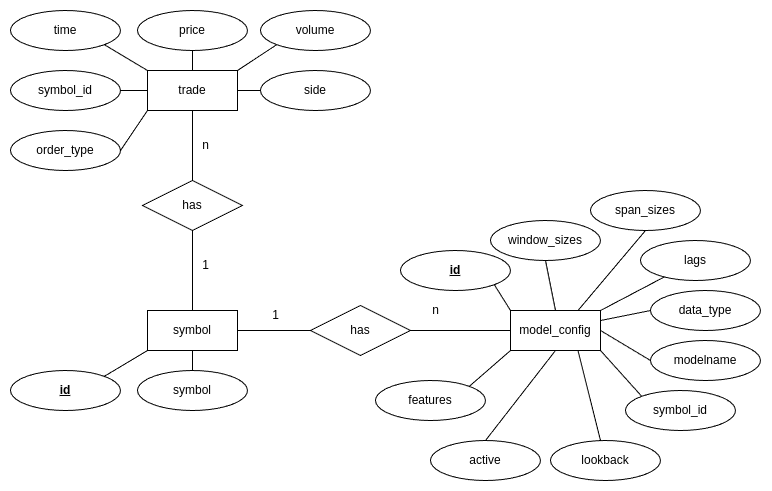
\includegraphics[width=\textwidth]{figures/ER-diagram.png}
    \caption{ER Diagram}
    \label{fig:er_diagram}
\end{figure}

The Entity-Relationship (ER) diagram establishes the database schema, which is designed for the storage and analysis of financial transactions. At its core is the \texttt{trade} entity essential for the transactional attributes: time, price, volume, linked via a \texttt{symbol\_id} to the corresponding currency pair in the \texttt{symbol} entity. This entity, with its unique identifier and descriptive nomenclature, categorizes the trades according to the traded financial instruments.

Accompanying the transactional data is the \texttt{model\_config} entity, which contains the configuration parameters critical for the predictive models utilized by the model service. Attributes defining the data's dimensions and historical scope, such as \texttt{span\_sizes}, \texttt{window\_sizes}, and \texttt{lags}, are specified to define the data features fed into the prediction models. The \texttt{model\_config's} direct association with the \texttt{symbol\_id} provides a unique configuration for each currency pair, facilitating the direct link between the predictive model and the financial instrument.

\subsection{Symbol Table}
The \texttt{symbol} table is defined as followed (Listing \ref{lst:symbol_table}), capturing the currency pairs.

\begin{lstlisting}[language=sql, caption=Symbol Table Structure, label=lst:symbol_table]
CREATE TABLE IF NOT EXISTS symbol (
    id SERIAL PRIMARY KEY,
    symbol TEXT NOT NULL UNIQUE
);

CREATE INDEX idx_symbol_symbol ON symbol (symbol);
\end{lstlisting}

This standard PostgreSQL table maintains a list of currency pairs like \texttt{ETH/USD}. An index is constructed to enhance the efficiency of queries, particularly when determining the associated \texttt{symbol\_id}.

\subsection{Model Configuration Table}
The structure of the \texttt{model\_config} table is delineated below (Listing \ref{lst:model_config_table}), encompassing the predictive model configurations:

\begin{lstlisting}[language=sql, caption=Model Configuration Table Structure, label=lst:model_config_table]
CREATE TABLE model_config (
    id SERIAL PRIMARY KEY,
    symbol_id SERIAL REFERENCES symbol(id),
    modelname TEXT,
    data_type TEXT,
    lookback INTEGER,
    lags INTEGER[],
    window_sizes INTEGER[],
    span_sizes INTEGER[],
    active BOOLEAN,
    features TEXT[]
);

ALTER TABLE model_config ADD CONSTRAINT model_config_constraint
UNIQUE (symbol_id, active);
\end{lstlisting}

This table not only records the configurations but also establishes a foreign key to the \texttt{symbol} table. A significant addition to the table is the unique constraint \texttt{model\_config\_constraint}, ensuring that only one configuration per \texttt{symbol\_id} can be marked as active at any given time. This enforces the exclusivity of active configurations, preventing conflicts and ambiguity in the model service operation. \\

The structure of the \texttt{trade} table  will be discussed in Section \ref{section:trade_table}, which focuses on hypertables. \\

In summary, the presented schema combines the transactional data with the intricacies of analytical model configurations, constructing a sophisticated data infrastructure for comprehensive financial analysis within the database.

\subsection{Hypertables}
Timescale introduces the concept of hypertables, a sophisticated abstraction over regular PostgreSQL tables specifically designed to enhance the management of time-series data. 

\begin{itemize}
    \item \textbf{Seamless Integration:} Hypertables blend in seamlessly with standard PostgreSQL tables, offering a dual-structure setup where each serves its distinct purpose. Users interact with hypertables just like regular tables, ensuring a familiar interface. This setup allows for efficient management of time-based data while maintaining the integrity and functionality of standard relational data storage.
    \item \textbf{Performance Optimization:} One of the primary advantages of hypertables is their ability to significantly improve insert and query performance. This is achieved through partitioning the time-series data based on the time dimension. Timescale efficiently manages the partitioning process behind the scenes, thereby abstracting the complexities involved in maintaining the hypertable's partitions.
\end{itemize}

In summary, hypertables in Timescale represent a pivotal innovation in the realm of time-series data management. They blend the familiarity of PostgreSQL tables with advanced time-based partitioning features, resulting in a powerful tool for efficient and effective time-series data handling.

\subsubsection{Trade Table:}
\label{section:trade_table}
\begin{lstlisting}[language=sql, caption=Trade Hypertable, label={lst:trade_hypertable}]
CREATE TABLE IF NOT EXISTS trade (
    time TIMESTAMPTZ NOT NULL,
    price DOUBLE PRECISION NOT NULL,  
    volume DOUBLE PRECISION NOT NULL, 
    side VARCHAR(1),
    order_type VARCHAR(1),
    symbol_id SERIAL NOT NULL
);

CREATE INDEX idx_trade_symbol_id ON trade (time, symbol_id);

SELECT create_hypertable('trade', 'time', migrate_data => true);
\end{lstlisting}

\begin{itemize}
\item \textbf{time}: The timestamp of the trade, essential for time-series analysis.
\item \textbf{price}: The price at which the trade occurred.
\item \textbf{volume}: The volume of the trade.
\item \textbf{side}: A variable indicating the trade side (e.g. buy or sell).
\item \textbf{order\_type}: The type of order executed in the trade (e.g. limit or market order).
\item \textbf{symbol\_id}: A unique identifier for the traded symbol.
\end{itemize}

In the early stages of this project the price and volume were stored using the PostgreSQL Numeric type. This choice was initially made due to the high precision of the Numeric type, which is particularly suitable for financial data where accuracy is paramount. However, it was observed that while the Numeric type ensures precision, it is not the optimal choice to use in Timescale, especially in the context of time-series data \cite{timescale_best_practices}. \newline

The primary challenge with the Numeric type in Timescale arises from its impact on performance. The performance impact is particularly noticeable when executing continuous aggregates on larger datasets. Continuous aggregates are fundamental in time-series databases for efficient data analysis, but the use of the Numeric type significantly hampers the performance of these operations. The larger storage size and processing requirements of the Numeric type, as compared to \texttt{DOUBLE PRECISION}, contribute to this performance degradation. \newline

As a result of these insights, the data type for price and volume was transitioned to \texttt{DOUBLE PRECISION}. This change strikes a balance between the need for precision and performance, which is crucial for time-series analysis in Timescale. \newline

Furthermore, the choice of \texttt{TIMESTAMPTZ} for time-stamping the data aligns with the best practices recommended for Timescale hypertables. The \texttt{TIMESTAMPTZ} data type, which stores both timestamp and timezone information, is particularly well suited for time-series data as it ensures accurate representation and manipulation of time, considering the time zone differences. This is essential in financial applications where transactions may span multiple time zones and accurate time-stamping is critical for analysis and reporting. \newline

Another optimization was storing only the \texttt{symbol\_id} instead of the full symbol (e.g., \texttt{ETH/USD}) in the database, as it significantly reduces data redundancy and optimizes query performance by referencing a compact, unique identifier for each trading pair.  

% see source https://www.timescale.com/blog/best-practices-for-picking-postgresql-data-types/  

\paragraph{Rationale for using a Hypertable:}
\begin{itemize}
\item \textbf{Time-based Partitioning}: As trades are inherently time-stamped the hypertable efficiently partitions data based on time, facilitating faster query performance, especially for time-bound data retrievals.
\item \textbf{Scalability}: With continuous growth in the trade data table, hypertables offer scalable solutions to manage large volumes of data without compromising on performance.
\item \textbf{Optimized Queries}: The creation of an index on the time and symbol\_id columns significantly enhances the query performance, especially for operations like range queries, which are common in financial analyses.
\item \textbf{Aggregation Support}: Hypertables are adept at handling aggregations, which are crucial for calculating OHLC (open, high, low, close) metrics, volume, and trade counts from raw trade data.
\end{itemize}

In essence, the utilization of a hypertable for the trade table in Timescale aligns with the requirements of time-series data handling in financial contexts. It provides an efficient, scalable, and performance-optimized framework for storing and querying trade data, thereby supporting intricate financial analysis and reporting.

\subsection{Materialized Views and Continuous Aggregates}

In the realm of time-series data management, especially in financial databases where data is voluminous and frequently accessed, optimizing query performance is crucial. Materialized Views and Continuous Aggregates in Timescale offer a potent solution for this challenge. These tools enable efficient data aggregation and faster retrieval by storing query results and refreshing them at regular intervals. This approach is particularly beneficial in scenarios involving repetitive and computationally intensive queries, such as aggregating trade data into OHLC (Open, High, Low, Close) metrics.

\subsubsection{OHLC Hourly Aggregation}
\label{section:ohlc_hourly_agg}
A materialized view named \texttt{ohlc\_hour} (Listing \ref{lst:ohlc_hour_materialized_view}) is utilized to aggregate trade data into hourly OHLC metrics. The view is created with the following characteristics:

\begin{lstlisting}[language=sql, caption=OHLC Materialized View, label={lst:ohlc_hour_materialized_view}]
CREATE MATERIALIZED VIEW ohlc_hour
WITH (timescaledb.continuous, timescaledb.create_group_indexes=TRUE, timescaledb.finalized=TRUE) AS
    SELECT
        time_bucket('1 hour', time) AS bucket,
        symbol_id,
        FIRST(price, time) AS open_price,
        MAX(price) AS high, 
        MIN(price) AS low,
        LAST(price, time) AS close_price,
        SUM(volume) AS volume,
        CAST(COUNT(*) AS INTEGER) AS count 
    FROM trade
GROUP BY bucket, symbol_id; 
\end{lstlisting}
\mbox{} \\
Key aspects of this view include:
\begin{itemize}
\item \textbf{Time Bucketing}: Aggregating trades into one-hour intervals.
\item \textbf{Data Accuracy}: The \texttt{finalized=TRUE} setting ensures that only fully aggregated data (complete hours) are returned.
\item \textbf{Trade Metrics}: Calculating open-, high-, low-, close-price, total volume, and trade count for each symbol within each time bucket.
\item \textbf{Overflow Consideration}: The trade count is cast to an integer, which has the potential for an overflow if the trade volume is exceedingly high, but after the analysis of the \texttt{ETH/USD} trades from the last couple of years the highest trade count in one hour was 25.000 trades which is nowhere close to the largest integer value of 2147483647.
\end{itemize}

Overall this materialized view reduces the raw trade data into a more manageable presentation, which will be utilized as a dataset for training the prediction models. 

\subsubsection{Continuous Aggregate Policy}
To maintain and update the \texttt{ohlc\_hour} view, a continuous aggregate policy is implemented (Listing \ref{lst:ohlc_hour_continuous_aggregate_policy}).

\begin{lstlisting}[language=sql, caption=OHLC Continuous Aggregate Policy, label={lst:ohlc_hour_continuous_aggregate_policy}]
SELECT add_continuous_aggregate_policy('ohlc_hour',
    start_offset => INTERVAL '3 hour', 
    end_offset => INTERVAL '1 hour',
    schedule_interval => INTERVAL '1 hour');
\end{lstlisting}
\mbox{} \\
This policy dictates:
\begin{itemize}
\item \textbf{Data Freshness}: Data is aggregated and refreshed every hour.
\item \textbf{Time Offsets}: Determines the range of data being aggregated, ensuring timely updates without processing very recent data that may still be incomplete.
\end{itemize}

Through the implementation of Materialized Views and Continuous Aggregates, the database efficiently processes and provides quick access to vital financial metrics, enhancing the system's performance and responsiveness for time-series analysis.

\subsection{Procedures and Functions}
\subsubsection{Symbol}
Efficient symbol management within the database is facilitated through the implementation of specialized functions, particularly the \texttt{insert\_symbol} function (Listing \ref{lst:insert_symbol_function}). This function is pivotal for insertion of new symbols into the \texttt{symbol} table and retrieving their identifiers.

\begin{lstlisting}[language=SQL, caption={Function for Inserting New Symbols}, label={lst:insert_symbol_function}]
CREATE OR REPLACE FUNCTION insert_symbol(input_symbol TEXT)
RETURNS TABLE(out_id INTEGER, out_symbol TEXT)
LANGUAGE plpgsql AS $$
BEGIN
    -- Attempt to insert the new symbol
    INSERT INTO symbol (symbol)
    VALUES (input_symbol)
    ON CONFLICT (symbol) DO NOTHING
    RETURNING id INTO out_id;
    -- If insertion did not occur due to a conflict, select the existing symbol
    IF NOT FOUND THEN
        RETURN QUERY SELECT id, symbol FROM symbol WHERE symbol = input_symbol;
    ELSE
        -- Set output symbol as the input symbol and return the record
        out_symbol := input_symbol;
        RETURN NEXT;
    END IF;
END;
$$;
\end{lstlisting}
\mbox{} \\
The function operates under two scenarios:
\begin{itemize}
    \item On receiving a new symbol, it attempts an insertion. If successful, the function returns the identifier of the newly inserted symbol.
    \item If the symbol pre-exists, indicated by a conflict, the function refrains from insertion and instead queries the identifier of the existing symbol.
\end{itemize}

Utilizing the \texttt{ON CONFLICT} clause ensures that the database maintains unique symbols, thus preserving data integrity. This function exemplifies the database's capability to manage symbols efficiently by preventing duplicate entries and streamlining the insertion process.


\subsubsection{Insert Trade Procedure}
To facilitate the addition of new trade data into the database, the \texttt{insert\_trade} procedure (Listing \ref{lst:insert_trade_procedure}) is implemented, which  is crucial for the collector service to insert trade transactions efficiently. 
\begin{lstlisting}[language=SQL, caption={Procedure for Inserting Trade Data}, label=lst:insert_trade_procedure]
CREATE OR REPLACE PROCEDURE insert_trade (
    _time TIMESTAMPTZ,
    _price DOUBLE PRECISION,  
    _volume DOUBLE PRECISION, 
    _side VARCHAR(1),
    _order_type VARCHAR(1),
    _symbol_id INTEGER 
)
LANGUAGE plpgsql AS $$
BEGIN
    INSERT INTO trade (time, price, volume, side, order_type, symbol_id) 
    VALUES (_time, _price, _volume, _side, _order_type, _symbol_id);
END;
$$;
\end{lstlisting}

This procedure requires trade-related parameters such as the timestamp, price, volume, trade side, order type, and the associated symbol identifier. Upon invocation, it performs a straightforward insertion of the provided data into the \texttt{trade} table. \\

Key Features:
\begin{itemize}
    \item \textbf{Efficiency in Data Entry}: By encapsulating the insertion logic within a procedure, the process of adding new trades to the database is streamlined, ensuring rapid and error-free data entry.
    \item \textbf{Parameterized Inputs}: The procedure utilizes parameterized inputs, which not only enhance the clarity of the data being inserted but also aid in maintaining consistency and data integrity.
\end{itemize}

The \texttt{insert\_trade} procedure plays an integral role in managing the influx of trade data, ensuring that the database is continuously updated with the latest transaction information.

\subsubsection{Get Trades Range Function}
The \texttt{get\_trades\_range} function (Listing \ref{lst:get_trades_range_function}) is an essential component of the database, designed to query trade data within a specified time range for a particular symbol. This function is particularly useful for analysis and reporting purposes where data needs to be filtered based on the time and symbol\_id. 
\begin{lstlisting}[language=SQL, caption={Function for Retrieving Trades Within a Specified Range}, label={lst:get_trades_range_function}]
CREATE OR REPLACE FUNCTION get_trades_range (
    input_from_date TIMESTAMPTZ,
    input_to_date TIMESTAMPTZ,
    input_symbol_id INTEGER 
)
RETURNS TABLE (
    time_ TIMESTAMPTZ,
    price DOUBLE PRECISION,
    volume DOUBLE PRECISION,
    side VARCHAR(1),
    order_type VARCHAR(1), 
    symbol_id INTEGER
)
LANGUAGE plpgsql AS $$
BEGIN
    RETURN QUERY
    SELECT
        trade.time,
        trade.price,
        trade.volume,
        trade.side,
        trade.order_type, 
        trade.symbol_id
    FROM trade 
    WHERE trade.symbol_id = input_symbol_id 
    AND trade.time >= input_from_date
    AND input_to_date >= trade.time
    ORDER BY trade.time; 
END;
$$;
\end{lstlisting}
\mbox{} \\
Features of the \texttt{get\_trades\_range} function include:
\begin{itemize}
    \item \textbf{Time-Range Query}: Allows querying of trade data between \texttt{input\_from\_date} and \texttt{input\_to\_date}, enabling precise temporal data retrieval.
    \item \textbf{Symbol-Specific Retrieval}: By accepting \texttt{input\_symbol\_id} as a parameter, the function filters trades related to a specific symbol, making it highly efficient for focused data analysis.
    \item \textbf{Structured Output}: A table consisting of trade timestamps, prices, volumes, sides, order types, and symbol\_ids is returned, offering a comprehensive view of the trade data.
    \item \textbf{Ordered Results}: The output is ordered by trade time, providing a chronological sequence of trades.
\end{itemize}

The \texttt{get\_trades\_range} function thus serves as a powerful tool for extracting relevant trade data, tailored to specific analytical requirements, and contributes significantly to the overall data querying capabilities of the database.

\subsubsection{Get OHLC Hour Range Function}
In order to facilitate the retrieval of aggregated trade data, specifically for OHLC (Open, High, Low, Close) metrics over hourly intervals, the \texttt{get\_ohlc\_hour\_range} function (Listing \ref{lst:get_ohlc_hour_range_function}) is implemented, which is crucial for analyzing the hourly price movements of different trading symbols.
\begin{lstlisting}[language=SQL, caption={Function for Retrieving Hourly OHLC Data}, label={lst:get_ohlc_hour_range_function}]
CREATE OR REPLACE FUNCTION get_ohlc_hour_range (
    input_from_date TIMESTAMPTZ,
    input_to_date TIMESTAMPTZ,
    input_symbol_id INTEGER 
)
RETURNS TABLE (
    bucket TIMESTAMPTZ,
    close_price DOUBLE PRECISION,
    volume DOUBLE PRECISION,
    count INTEGER, 
    symbol_id INTEGER
)
LANGUAGE plpgsql AS $$
BEGIN
    RETURN QUERY SELECT 
        ohlc_hour.bucket,
        ohlc_hour.close_price,
        ohlc_hour.volume,
        ohlc_hour.count,
        ohlc_hour.symbol_id
    FROM ohlc_hour
    WHERE ohlc_hour.symbol_id = input_symbol_id
    AND ohlc_hour.bucket >= input_from_date  
    AND input_to_date >= ohlc_hour.bucket 
    ORDER BY ohlc_hour.bucket; 
END;
$$;
\end{lstlisting}
\mbox{} \\
Key functionalities of the \texttt{get\_ohlc\_hour\_range} function include:
\begin{itemize}
    \item \textbf{Time Interval Selection}: It allows querying of OHLC data between \texttt{input\_from\_date} and \texttt{input\_to\_date}, providing flexibility in selecting specific time ranges for analysis.
    \item \textbf{Symbol-Specific Aggregation}: Filters the data for a particular symbol, as specified by \texttt{input\_symbol\_id}, enabling focused examination of a single trading entity.
    \item \textbf{Data Aggregation}: Retrieves hourly aggregated data including the closing price, total volume, trade count, and the timestamp of each aggregation interval (`bucket`) from the materialized view \texttt{ohlc\_hour} (Listing \ref{lst:ohlc_hour_materialized_view})
    \item \textbf{Chronological Ordering}: The results are ordered by the \texttt{bucket} timestamp, offering a sequential view of the OHLC data for comprehensive analysis.
\end{itemize}

The \texttt{get\_ohlc\_hour\_range} function is thus instrumental in providing access to hourly aggregated trade data, a vital resource for detailed financial market analysis and trend identification. This function is also essential for the model service as this data is needed for the prediction model.

\subsubsection{Get Model Configuration Function}
Playing a crucial role for the model service, the \texttt{get\_model\_config} function (Listing \ref{lst:get_model_config_function}) is specifically designed to retrieve the configuration settings of predictive models associated with a given \texttt{symbol\_id}, which is essential for accessing model parameters that are active and relevant to a particular symbol. 
\begin{lstlisting}[language=SQL, caption={Function for Retrieving Model Configuration}, label={lst:get_model_config_function}]
CREATE OR REPLACE FUNCTION get_model_config (
    input_symbol_id INTEGER 
)
RETURNS TABLE (
    id INTEGER,
    symbol_id INTEGER,
    modelname TEXT,
    data_type TEXT,
    lookback INTEGER,
    lags INTEGER[],
    window_sizes INTEGER[],
    span_sizes INTEGER[],
    active BOOLEAN,
    features TEXT[]
)
LANGUAGE plpgsql AS $$
BEGIN
    RETURN QUERY SELECT 
        model_config.id,
        model_config.symbol_id,
        model_config.modelname,
        model_config.data_type,
        model_config.lookback,
        model_config.lags,
        model_config.window_sizes,
        model_config.span_sizes,
        model_config.active,
        model_config.features
    FROM model_config
    WHERE model_config.symbol_id = input_symbol_id 
    AND model_config.active IS TRUE;
END;
$$;
\end{lstlisting}
\mbox{} \\
Features and functionalities of the \texttt{get\_model\_config} function include:
\begin{itemize}
    \item \textbf{Symbol-Specific Retrieval}: It filters the model configurations based on the \texttt{input\_symbol\_id}, ensuring that the returned settings are specific to the requested symbol.
    \item \textbf{Active Configurations}: Only returns configurations that are marked as active (\texttt{active IS TRUE}), thereby providing parameters that are currently in use.
    \item \textbf{Comprehensive Configuration Data}: The returned table includes a wide range of configuration parameters such as model name, data type, lookback period, lags, window sizes, span sizes, and the features array, offering a detailed overview of the model settings.
\end{itemize}

\subsection{MlFlow Database}
For the integration of MLflow into the Timescale database, a separate database has been established specifically for storing model-related information generated by MLflow. This approach ensures that the data is organized and the system's components are neatly compartmentalized. The creation of this dedicated MLflow database is handled in the \texttt{create\_tables.sql} script (Listing \ref{lst:mlflow_database}).

\begin{lstlisting}[language=python, caption={Create MlFLow Datavase}, label={lst:mlflow_database}]
CREATE DATABASE mlflow;
\end{lstlisting}

\section{Model Development: Long Short-Term Memory}
\label{section:model_dev}

This section delves into the utilization of Long Short-Term Memory (LSTM) networks for time series forecasting, a topic that has attracted considerable attention in predictive analytics. As a specialized subclass of Recurrent Neural Networks (RNNs), LSTM networks are selected for their ability to effectively capture temporal dependencies in time series data. \\

While advanced deep learning techniques like Transformers and Autoformers are available, the choice to employ a LSTM model is influenced by its relative simplicity and straightforward setup process. Such an approach strikes a balance between complexity and performance, providing a feasible gateway to exploring deep learning methods in time series analysis. Nonetheless, it is crucial to recognize that LSTMs, despite being a notable improvement over traditional methods, is no silver bullet for time series forecasting and has it's own set of limitations. \\

A primary challenge encountered with LSTM is the handling of exceedingly long sequences, which may be hindered by memory and computational constraints. Moreover, although LSTMs are adept at identifying temporal dependencies, their effectiveness can vary across different time series datasets, especially those with intricate patterns or nonlinear relationships. \\

\subsection{Model Selection:}
The decision to employ Long Short-Term Memory (LSTM) networks for this thesis was driven by several key factors that align closely with the objectives and constraints of this framework. \\

\begin{itemize}
    \item \textbf{Proven Effectiveness in Time-Series Prediction:} LSTM networks are renowned for their ability to capture long-term dependencies and patterns in time-series data, a characteristic crucial for analyzing financial markets. Their architecture is specifically designed to address the challenges of sequential data, making them out to be the right tool for tasks like predicting cryptocurrency prices, which involve complex and time-sensitive patterns.
    \item \textbf{Widespread Usage and Community Support:} LSTM's popularity in various applications, especially in financial forecasting, means there is a wealth of literature, tutorials, and community support available. This abundance of resources facilitates easier implementation, troubleshooting, and optimization, which is particularly beneficial for newly emerging projects.
    \item \textbf{Simplicity and Accessibility:} Despite being a powerful deep learning tool, LSTMs are relatively straightforward to implement, especially with the availability of high-level machine learning libraries. This ease of use allows for quick setup and iteration, enabling the project to progress rapidly from the conceptual stage to practical testing and refinement.
    \item \textbf{Adaptability and Scalability:} LSTM networks are adaptable to a range of data inputs and structures, making them suitable for the diverse and evolving nature of cryptocurrency data. Additionally, their scalability ensures that the model can handle increasing data volumes and complexity as the framework evolves.
    \item \textbf{Strong Baseline for Future Enhancements:} Starting with a well-understood and established model like LSTM provides a solid foundation. It allows for the establishment of a reliable baseline, from which more complex or specialized models can be explored in future iterations.\\
\end{itemize}

In summary, the selection of LSTM is anchored in its proven track record in time-series analysis, its widespread adoption and support in the machine learning community, and its balance between sophistication and user-friendliness. These attributes made LSTM an ideal choice for this initial foray into the intricate world of cryptocurrency price prediction, providing a strong and adaptable platform for ongoing research and development. \\

\subsection{Data Preparation}
\label{section:data_preparation}
The foundation of an effective forecasting model lies in the quality and structure of the dataset used. For the development of the LSTM forecasting model, historical data from the Kraken cryptocurrency exchange for the currency pair \texttt{ETH/USD} has been utilized \cite{Kraken2023}. The initial dataset comprises of epoch millisecond timestamps, trading prices, and volumes. This format is consistent with the data collected by the collector (Section \ref{section:collector}), yet using such raw data presents challenges. Firstly, the considerable size of the raw dataset (33.9MB for only Q4 2023) makes processing cumbersome. Secondly, raw data often contains a significant amount of noise.  To address these issues, the data was aggregated into an hourly OHLC (open-, high-, low-, close-price) format. In addition to these metrics, volume and trade count were also included. This aggregation reduces noise and condenses the dataset into a more manageable form. \\ \mbox{} \\
The dataset was created using the \texttt{ohlc\_hour} materialized view (Section \ref{section:ohlc_hourly_agg}). First the historical data was imported through the frontend's data import functionality (Section \ref{section:frontend_upload}). For model training, the data was exported via pgAdmin (Section \ref{section:pgadmin_user_guide}), encompassing a limited time range, which best reflects the latest market patterns. This timeframe also limited the data set size to 32361 time-steps, which resulted in the following dataset structure (Table \ref{table:extended_time_series_data}): 
\mbox{}
\begin{table}[H]\small    
\centering
\begin{tabular}{|l|l|l|l|l|l|l|l|}
\hline
\textbf{bucket} & \textbf{id} & \textbf{open} & \textbf{high} & \textbf{low} & \textbf{close} & \textbf{volume} & \textbf{count} \\ \hline
2020-01-01 00:00:00+00 &1& 128.66 & 128.66 & 128.19 & 128.42 & 515.78081605 & 112 \\ \hline
2020-01-01 01:00:00+00 &1& 128.33 & 130.05 & 128.3 & 130.05 & 555.0542868099997 & 159 \\ \hline
... & ... & ... & ... &...& ... & ... & ...  \\ \hline
2023-09-30 22:00:00+00 &1& 1674.72 & 1677.35 & 1674.24 & 1675.23 & 95.91776195 & 201 \\ \hline
2023-09-30 23:00:00+00 &1& 1674.94 & 1674.95 & 1669.62 & 1671.01 & 158.58122506 & 210 \\ \hline
\end{tabular}
\caption{Training Dataset ETH/USD}
\label{table:extended_time_series_data}
\end{table}

\begin{figure}[H]
    \centering
    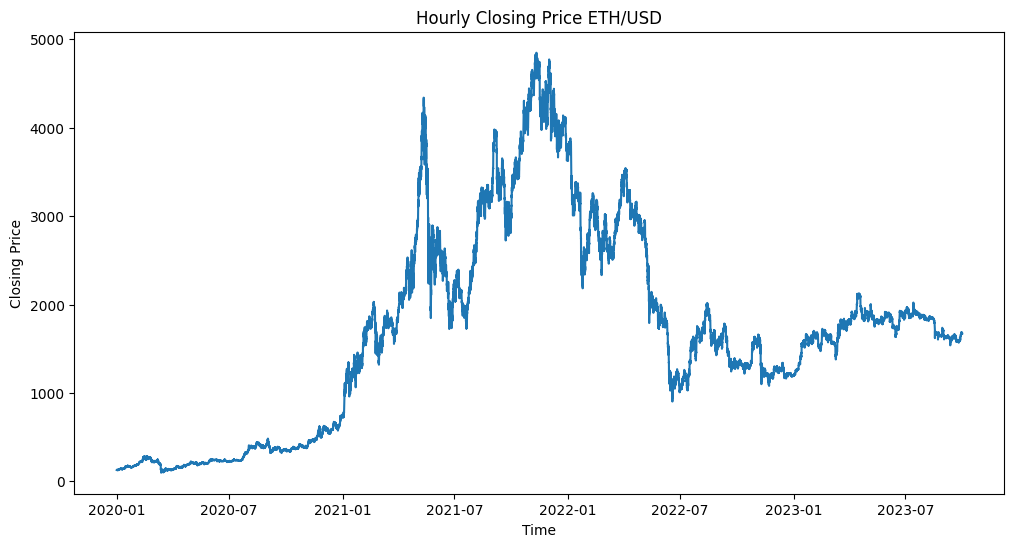
\includegraphics[width=0.93\textwidth]{figures/training_dataset_plot.png}
    \caption{Training Dataset (ETH/USD)}
    \label{fig:training_dataset_plot}
\end{figure}

The created dataset was then used for model tuning (Section \ref{section:model_tuning}), where it was loaded into a Pandas DataFrame. Pandas is a powerful data manipulation and analysis library for Python, which offers an extensive set of tools ideal for manipulating time series data \cite{PandasDocs}, providing a solid foundation for the subsequent feature engineering. 

\subsubsection{Date Time Feature}
\label{section:datetime_feature}

The \texttt{process\_timestamp} function (Listing \ref{lst:process_timestamp}) is designed to perform two key operations on the \texttt{bucket} column of the training dataset:

\begin{enumerate}
    \item \textbf{Conversion to Datetime Objects:}  The function starts by converting the values in the \texttt{bucket} column into datetime objects using the pandas \texttt{to\_datetime()} function. 
    \item \textbf{Handling Missing Data Points (Optional):} Offers an optional feature to handle gaps in the dataset. If the fill parameter is set to True, the function will execute a series of steps to fill in gaps. The dataset is resampled into one-hour intervals using \texttt{data.resample('h').asfreq()}. This step ensures that the time series data is uniformly spaced, creating a consistent time frame for analysis. The function then fills missing values in the \texttt{close\_price} column by carrying forward the last available value (forward fill). This method is chosen as it is a common practice in time series analysis, especially for financial data, where the most recent known value is often the best estimate for missing data. For the \texttt{volume} and \texttt{count} columns, missing values are filled with zeros. This choice reflects the assumption that a lack of data implies no trades or countable events occurred during that time period. 
\end{enumerate}

Finally, the dataset is sorted and reset to ensure that it is ordered correctly and the indices are consistent. \\

\begin{lstlisting}[language=python, caption={Processing timestamp}, label=lst:process_timestamp]
def process_timestamp(data, fill=False): 
    data['bucket'] = pd.to_datetime(data['bucket'])
    data.set_index('bucket', inplace=True)
    if fill: 
        data = data.resample('h').asfreq()
        data['close_price'] = data['close_price'].fillna(method='ffill')
        data['volume'] = data['volume'].fillna(0) 
        data['count'] = data['count'].fillna(0)
    data.sort_values('bucket', inplace=True)
    data.reset_index(inplace=True)
    return data
\end{lstlisting}

After preprocessing the timestamp is split up into hour, day of the week, day of the month, month and year using the \texttt{add\_feature\_date} function (\ref{lst:split_timestamp}. \\

\begin{lstlisting}[language=python, caption={Splitting timestamp}, label=lst:split_timestamp]
def add_feature_date(data):
    # time-based features
    data['hour'] = data['bucket'].dt.hour
    data['day_of_week'] = data['bucket'].dt.dayofweek #Monday=0, Sunday=6
    data['day_of_month'] = data['bucket'].dt.day
    data['month'] = data['bucket'].dt.month
    data['year'] = data['bucket'].dt.year
\end{lstlisting}

The reason for splitting the date and time is because LSTM networks require input features that effectively represent the temporal dynamics in the data. Cyclic encoding is a method used to transform time-related features into a format that preserves their cyclical nature, which is crucial for accurate time series forecasting. The functions \texttt{apply\_cyclic\_encoding} and \texttt{encode\_cyclic\_feature} are instrumental in this process. \\ 
% add a source here to back up why this is good

The \texttt{apply\_cyclic\_encoding} function (Listing \ref{lst:apply_cyclic_encoding}) applies cyclic encoding to specified time-related columns in the dataset. This function takes two parameters: the dataset and a list of columns to apply the encoding to. For each column, it uses the \texttt{get\_distinct\_count} function to determine the length of the cycle (e.g., 24 for hours, 7 for days of the week) and then applies the \texttt{encode\_cyclic\_feature} function to create two new columns for each feature, representing the sine and cosine components of the cyclic encoding.

\begin{lstlisting}[language=python, caption={Applying cyclic encoding}, label=lst:apply_cyclic_encoding]
def apply_cyclic_encoding(data, columms=['hour','day_of_week','month']): 
    for column in columms: 
        cycle_length = get_distinct_count(data, column)
        data[column + "_cos"] = data[column].apply(lambda x: encode_cyclic_feature(x, cycle_length, type='cos')).astype(float)
        data[column + "_sin"] = data[column].apply(lambda x: encode_cyclic_feature(x, cycle_length, type='sin')).astype(float)
    return data
\end{lstlisting}

The \texttt{encode\_cyclic\_feature} function (Listing \ref{lst:encode_cyclic_feature}) takes a single value, the cycle length of the feature, and the type of encoding (sin or cos). It converts the value into radians and then applies either the sine or cosine function. This conversion to a circular format enables the model to recognize that the end of one cycle connects back to the beginning (e.g., the 23rd hour connects back to the 0th hour). The encoding's outcome is illustrated with the \texttt{day\_of\_the\_month} feature, displaying data for the entire year of 2016, as seen in Figure \ref{fig:day_month_encoding}. \\

\begin{lstlisting}[language=python, caption={Encoding cyclic feature}, label=lst:encode_cyclic_feature]
def encode_cyclic_feature(value, cycle_length, type):
    value_rad = (value / cycle_length) * 2 * np.pi
    if type == 'sin':
        return np.sin(value_rad) 
    else: 
        return np.cos(value_rad)
\end{lstlisting}

This encoding is important because for example, hours of the day or days of the week recur in a predictable pattern. By encoding these features as sine and cosine values (Figure \ref{fig:day_month_encoding}), the LSTM can better understand and utilize the periodicity in the data, which in turn should lead to more accurate time series predictions. \\

\textbf{Special Cyclic Encoding for Day of the Month:} \\
The functions \texttt{encode\_day\_of\_month} and \texttt{apply\_day\_of\_month\_encoding} (Listings \ref{lst:encode_day_of_month_feature} \& \ref{lst:apply_day_of_month_feature}) are designed to address the cyclic nature of days in a month, considering the varying lengths of different months. \\

The \texttt{encode\_day\_of\_month} function (Listing \ref{lst:encode_day_of_month_feature}) takes the day of the month, month, and year as inputs and normalizes the day of the month based on the total number of days in a given month. This normalization accounts for the alternating number of days in different months and the edge case of February. The function then applies a cyclic encoding (sine and cosine) to this normalized value. This encoding effectively maps each day to a point on a circle, thus preserving the cyclical pattern of days within a month.

\begin{lstlisting}[language=python, caption={Encoding Day of the Month feature}, label=lst:encode_day_of_month_feature]
def encode_day_of_month(day_of_month, month, year, type):
    normalized_day = (day_of_month - 1) / get_month_length(month, year)  # Subtract 1 to start from 0
    if type == 'sin': 
        return np.sin(2 * np.pi * normalized_day) 
    else: 
        return np.cos(2 * np.pi * normalized_day) 
\end{lstlisting}

The \texttt{apply\_day\_of\_month\_encoding} function (Listing \ref{lst:apply_day_of_month_feature}) applies the \\\texttt{encode\_day\_of\_month} function to each row in the dataset. It adds two new columns, \texttt{day\_of\_month\_sin} and \texttt{day\_of\_month\_cos}, representing the sine and cosine cyclic encoding of the day of the month. This approach ensures that the model recognizes the continuity from the end of one month to the beginning of the next.

\begin{lstlisting}[language=python, caption={Applying Day of the Month Encoding}, label=lst:apply_day_of_month_feature]
def apply_day_of_month_encoding(data): 
    data["day_of_month_sin"] = data.apply(lambda row: encode_day_of_month(row['day_of_month'], row['month'], row['year'], 'sin'), axis=1)
    data["day_of_month_cos"] = data.apply(lambda row: encode_day_of_month(row['day_of_month'], row['month'], row['year'], 'cos'), axis=1)
    return data
\end{lstlisting}

This specialized encoding is crucial for LSTM models that forecast based on date-time data. Standard representations of dates might not effectively convey the cyclic nature of time, particularly for features like the day of the month that do not have a fixed cycle length. By using this cyclic encoding, LSTM models can better capture and utilize the temporal dynamics inherent in the data, leading to potentially more accurate and meaningful predictions, especially in scenarios where the day of the month has a significant impact on the observed time series data (e.g. consumer behavior, financial market trends, etc.). \\

\begin{figure}[H]
    \centering
    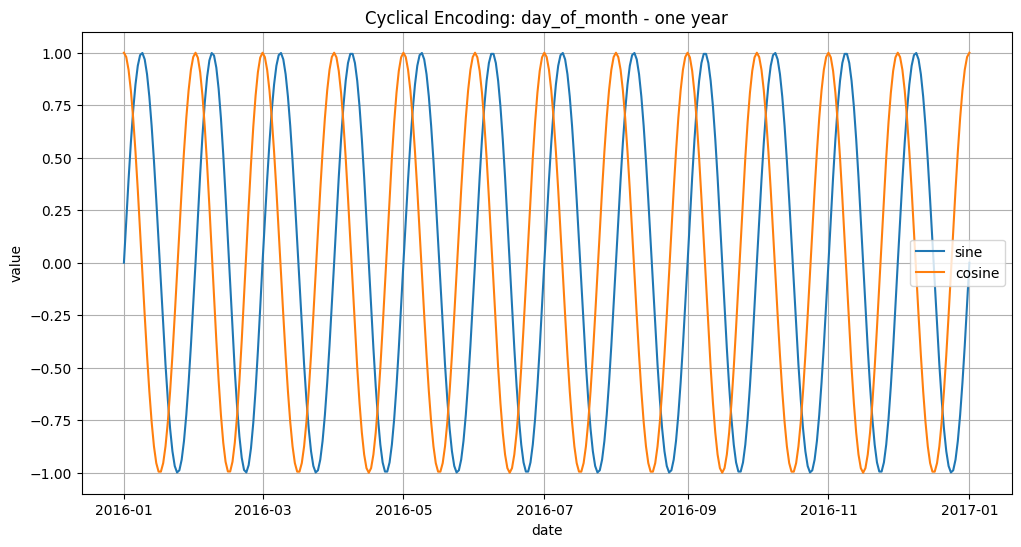
\includegraphics[width=\textwidth]{figures/day_of_the_month_encoding.png}
    \caption{Day of the Month Encoding}
    \label{fig:day_month_encoding}
\end{figure}

\subsubsection{Normalization of the Year Feature}
In time series analysis, particularly when preparing data for LSTM models, normalizing features can be critical to model performance. The function \texttt{normalize\_year} is designed to normalize the \texttt{year} column in the dataset. 
The \texttt{normalize\_year} function (Listing \ref{lst:year_normalization}) takes a dataset and an optional list of column names (defaulting to ['year']). For each specified column, it calculates the minimum and maximum values using the \texttt{get\_min\_max\_value} function. Then, it applies a normalization formula to each value in the column, scaling it to a range between 0 and 1. This normalization is achieved by subtracting the minimum value from the column value and dividing by the range (max - min + 1). The '+1' in the denominator is specifically added to account for the year 2024, ensuring that the scale includes the entire range of years present in the data plus one additional year.

\begin{lstlisting}[language=python, caption={Year normalization}, label=lst:year_normalization]
def normalize_year(data, columns=['year']): 
    for column in columns: 
        min, max = get_min_max_value(data, column)
        data[column+'_normalized'] = data[column].apply(lambda x: normalize_feature(x, min, max+1)) # +1 to account for 2024
    return data
\end{lstlisting}
\mbox{}\\
\paragraph{Importance of Normalization:}
Normalization of the year is crucial for several reasons:
\begin{itemize}
    \item \textbf{Consistency in Scale:} Normalizing ensures that the \texttt{year} feature has a consistent scale compared to other features in the dataset, which is essential for models like LSTMs that are sensitive to the scale of the input data.
    \item \textbf{Improved Model Training:} Features on a similar scale can lead to faster convergence during training, as it helps in maintaining numerical stability and a balanced gradient flow.
\end{itemize}

In summary, the \texttt{normalize\_year} function provides a method to scale the year feature appropriately, enhancing its utility for LSTM models, where scale and continuity of data are key factors for model accuracy and performance.

\subsubsection{US-Holidays Feature}
In the realm of time series forecasting, especially in financial markets, recognizing special calendar events like holidays can be crucial. The function \texttt{add\_holiday\_feature} (Listing \ref{lst:holiday}) is designed to integrate this aspect into the dataset.

\begin{lstlisting}[language=python, caption={US-Holidays feature}, label={lst:holiday}]
def add_holiday_feature(data):
    us_holidays = holidays.UnitedStates()
    data['is_holiday'] = data['bucket'].apply(lambda x: x in us_holidays).astype(int)
    return data
\end{lstlisting}

The \texttt{add\_holiday\_feature} function (Listing \ref{lst:holiday}) introduces a binary feature \\ \texttt{is\_holiday} to the dataset. It utilizes the holidays library to create a list of US holidays and then applies a lambda function to the bucket column, which stores the timestamps. For each timestamp, the function checks whether the date is a US holiday. If so, the \texttt{is\_holiday} column is marked with a 1, otherwise a 0. This binary encoding effectively differentiates regular days from US holidays. 

\paragraph{Potential Impact:}
The inclusion of the \texttt{is\_holiday} feature provides the LSTM model with additional context about the timing of data points. Holidays can impact financial markets in various ways, such as reduced trading volume or closure of markets, which in turn can affect the price movement of assets. By providing this information, the model might be able to better anticipate and account for these irregularities in the data.
However, it is important to consider the global nature of cryptocurrency trading when evaluating the impact of this feature. The \texttt{ETH/USD} market, like other cryptocurrency markets, operates worldwide and is not confined to a single timezone or region. Therefore, while US holidays might have some influence, their impact could be less pronounced compared to traditional markets that are more regionally focused. This means that while the \texttt{is\_holiday} feature could contribute to the model's understanding of certain market behaviors, its overall influence on a global and decentralized market like \texttt{ETH/USD} might be overvalued.

\subsubsection{Logarithmic Scaling}

Applying appropriate transformations to the input features is crucial for optimizing the performance of LSTM models in time series analysis. The \texttt{apply\_log\_scaler} function is designed to apply a logarithmic transformation to specific features in the dataset. \\

The \texttt{apply\_log\_scaler} function (Listing \ref{lst:log_scaler}) takes a dataset and a list of column names (defaulting to ['close\_price', 'volume', 'close\_lag12', 'close\_lag168']). For each column in this list, it applies the natural logarithm transformation using the \texttt{np.log1p} (numpy) function. This function computes the natural logarithm of one plus the input value, effectively scaling the data while also handling zero values gracefully. \\

\begin{lstlisting}[language=python, caption={Logarithmic Scaling Function}, label=lst:log_scaler]
def apply_log_scaler(data, columns=['close_price', 'volume', 'close_lag12', 'close_lag168']): 
    for column in columns:
        data[column] = np.log1p(data[column])
    return data
\end{lstlisting}

\paragraph{Importance of Logarithmic Scaling}
Logarithmic scaling is particularly beneficial in time series forecasting for several reasons:
\begin{itemize}
    \item \textbf{Handling Skewed Data:} A lot of financial time series data, like prices and volumes, can be highly skewed. Logarithmic scaling helps in reducing this skewness, making the data distribution more symmetrical and thus more suitable for LSTM models.
    \item \textbf{Stabilizing Variance:} This transformation tends to stabilize the variance across the data, which can be highly beneficial for models that assume constant variance in the input features.
    \item \textbf{Multiplicative to Additive:} Converts multiplicative relationships into additive ones, which can be easier for models like LSTMs to learn and capture in their predictions.
\end{itemize}

\paragraph{Selection of Features:}
The choice of features for logarithmic scaling (eg.: 'close\_price', 'volume', 'close\_lag12', 'close\_lag168', 'count') is based on their characteristics in financial time series data. These features often exhibit exponential growth or decay, and logarithmic scaling can transform them into a more linear relationship. This can be beneficial for the learning process of LSTM networks. \\

In conclusion, the \texttt{apply\_log\_scaler} function plays a vital role in preprocessing the data for LSTM models, particularly in financial time series analysis, by transforming key features to a form that is more conducive to the learning and predictive capabilities of these models.

\subsubsection{Lag Feature}

Lag features are a critical component in time series forecasting, particularly when using LSTM models that are designed to capture temporal dependencies. The \texttt{add\_feature\_lag} function adds these lag features to the dataset, enhancing the model's ability to learn from past data. \newline

The \texttt{add\_feature\_lag} function (Listing \ref{lst:lag_feature}) takes a dataset and a list of integers representing the lags to be created. For each lag in the list it creates a new column in the dataset, labeled \texttt{close\_lag} followed by the lag number. This new column contains the close\_price feature shifted by the number of time steps specified by the lag. This shift means that each new \texttt{close\_lagX} column contains the close\_price from X time steps in the past.

\begin{lstlisting}[language=python, caption={Lag Feature}, label=lst:lag_feature]
def add_feature_lag(data, lags=[1]): 
    for lag in lags: 
        data['close_lag'+str(lag)] = data['close_price'].shift(lag)
    return data
\end{lstlisting}

\paragraph{Importance of Lag Features}
Lag features are vital in time series analysis for several reasons:
\begin{itemize}
    \item \textbf{Capturing Temporal Dependencies:} They allow the model to access past values of the time series, which is essential for capturing patterns and trends over time.
    \item \textbf{Enhancing Forecast Accuracy:} By providing the model with historical data points, lag features can significantly improve the accuracy of forecasts.
    \item \textbf{Flexibility in Model Design:} Different lags can capture different aspects of temporal dynamics, allowing for a more nuanced and comprehensive model.
\end{itemize}

In summary, the \texttt{add\_feature\_lag} function provides a simple yet powerful way to enrich a time series dataset with past information, enabling LSTM models to make more informed predictions.

\subsubsection{Moving Averages}

Moving averages are a foundational tool in time series analysis, particularly in financial markets where they help in identifying trends and smoothing out short-term fluctuations. The functions \texttt{simple\_moving\_average} and \texttt{exponential\_moving\_average} add these moving average features to the dataset. \\

The \texttt{simple\_moving\_average} function (Listing \ref{lst:sma}) computes the simple moving average (SMA) for specified columns over given window sizes. For each column and window size, it creates a new column in the dataset labeled \texttt{sma\_WINDOWSIZE\_COLUMN}, where \texttt{WINDOWSIZE} is the size of the moving window, and \texttt{COLUMN} is the name of the original column. The SMA is calculated by averaging the values of the column over the specified window size. \\

Similarly, the \texttt{exponential\_moving\_average} function (Listing \ref{lst:ema}) calculates the exponential moving average (EMA) for the specified columns. EMA gives more weight to recent data points, making it more responsive to new information. For each column and span size, it adds a new column labeled \texttt{ema\_SPAN\_COLUMN}. The span size determines the rate at which older observations are weighted down. \\

\begin{lstlisting}[language=python, caption={Simple Moving Average Feature}, label={lst:sma}]
def simple_moving_average(data, window_sizes, columns=['close_price']): 
    for column in columns: 
        for window_size in window_sizes: 
            data['sma_'+str(window_size)+"_"+column] = data[column].rolling(window=window_size).mean()
    return data
\end{lstlisting}

\begin{lstlisting}[language=python, caption={Exponential Moving Average Feature}, label={lst:ema}]
def exponential_moving_average(data, span_sizes,columns=['close_price']):
    for column in columns: 
        for span in span_sizes: 
            data['ema_'+str(span)+"_"+column] = data[column].ewm(span=span).mean()
    return data
\end{lstlisting}

\paragraph{Importance of Moving Averages}
Moving averages are especially useful in the context of LSTM models for several reasons:
\begin{itemize}
    \item \textbf{Data Smoothing:} They help in smoothing out random fluctuations in the data, highlighting underlying trends, which can be beneficial for LSTMs in capturing long-term dependencies.
    \item \textbf{Trend Identification:} Moving averages can assist the model in identifying and adapting to trends in the data, which is vital in forecasting tasks.
    \item \textbf{Re-activeness to Recent Changes:} EMAs can provide a more reactive feature that responds quickly to recent changes in the data, potentially improving the model's ability to predict short-term movements.
\end{itemize}

\paragraph{Application in Financial Time Series:}
In financial time series forecasting, such as stock or cryptocurrency prices, moving averages are instrumental in understanding market behavior. They can act as indicators of potential support and resistance levels, trend directions, and momentum, which can be crucial inputs for an LSTM model aiming to predict future price movements.

In conclusion, the \texttt{simple\_moving\_average} and \texttt{exponential\_moving\_average} functions enrich the dataset with essential trend-based features, enhancing the predictive capabilities of LSTM models in time series analysis.

% dataset: https://support.kraken.com/hc/en-us/articles/360047543791-Downloadable-historical-market-data-time-and-sales-

\subsection{Model Tuning}
\label{section:model_tuning}

Effective model tuning is pivotal in the development of robust and accurate forecasting models. This section delves into the intricate process of fine-tuning the Long Short-Term Memory (LSTM) network, specifically tailored for time series forecasting of the \texttt{ETH/USD} currency pair. The focus is on leveraging a comprehensive parameter grid to systematically explore a multitude of feature combinations and model configurations. This systematic approach ensures a thorough exploration of the parameter space, leading to an optimized model that can effectively capture the complexities of the time series data. \\

Central to this process is the utilization of MLflow, a versatile platform for managing the machine learning lifecycle, including experimentation, reproducibility, and deployment. MLflow plays a critical role in tracking experiments, enabling an organized and efficient review of model performance across different configurations. The ability to log and compare various parameters, metrics, and models streamlines the model selection process and fosters a methodical approach to model tuning. \\

\subsubsection{Setting Up the Model Tuning Environment}

The model tuning process is orchestrated within a Jupyter Notebook, which serves as an interactive computational environment for running the tuning script. This setup not only facilitates an intuitive and flexible way to run complex analyses but also allows for immediate visualization and interaction with the data and models. \\

A crucial aspect of this setup is the integration with various services, managed through Docker containers, to streamline the model tracking and data storage processes. The Jupyter Notebook is configured to interact with the following services. \\

\begin{itemize}
    \item \textbf{MLflow Docker Container:} The MLflow tracking server is set up in a Docker container (Section \ref{section:mlflow_docker}). By setting the MLflow tracking URI to \url{http://127.0.0.1:5000}, the Jupyter Notebook connects to the MLflow server running locally within the Docker container. This connection allows for the systematic tracking of experiments, including logging parameters, metrics, and models.

    \item \textbf{MinIO Docker Container:} MinIO (Section \ref{section:minio}) is utilized for storing artifacts related to the machine learning experiments. The Jupyter Notebook is configured to interact with the MinIO server through specified AWS credentials and the S3 endpoint URL. The AWS credentials \texttt{AWS\_ACCESS\_KEY\_ID} and \texttt{AWS\_SECRET\_ACCESS\_KEY} are set as environment variables. Additionally, the \texttt{MLFLOW\_S3\_ENDPOINT\_URL} environment variable is set to the MinIO server's address, \url{http://172.1.0.12:2000}, enabling the storage and retrieval of MLflow artifacts within the MinIO storage.

    \item \textbf{PostgreSQL Database:} PostgreSQL (Section \ref{section:timescale_docker}) is employed to store model tracking information. The integration with PostgreSQL allows for efficient management and querying of experiment data, enhancing the ability to analyze and compare different model versions and configurations.
\end{itemize}

This environment setup provides a robust and scalable framework for model tuning, ensuring that all aspects of the machine learning process, from experiment tracking to artifact storage, are meticulously managed and easily accessible.\\

\begin{lstlisting}[language=python, caption={Model Tuning Evnironment Setup}, label={lst:model_tuning_environment}]
os.environ["AWS_ACCESS_KEY_ID"] = "eITEO5kyE7hccuy7UTHv"
os.environ["AWS_SECRET_ACCESS_KEY"] = 
    "5KBCscit30Z70bSVGIMvMBBoqV8ydn232o2MW9RA"
os.environ["MLFLOW_S3_ENDPOINT_URL"] = f"http://172.1.0.12:2000"

mlflow.set_tracking_uri(uri="http://127.0.0.1:5000")
\end{lstlisting}

\subsubsection{Construction of the Parameter Grid}

In the model tuning phase, a comprehensive parameter grid is constructed to systematically evaluate different combinations of features and LSTM model hyperparameters, which is essential to optimize the model's performance.

\paragraph{Feature Combinations}
The parameter grid begins with the specification of fixed and optional features. Fixed features include essential time-related attributes like 'hour', 'day of week', 'month', 'day of month', normalized 'year', as well as other relevant features such as 'is\_holiday', 'volume', 'is\_weekend', 'count', and 'close\_price'. These features are considered crucial for capturing the fundamental temporal patterns in the time series data. \\

\begin{lstlisting}[language=python, caption={Model Tuning Fixed and Optional Features}, label={lst:model_tuning_fixed_optional_features}]
fixed_features = ['hour_cos', 'hour_sin', 'day_of_week_cos',
    'day_of_week_sin', 'month_cos', 'month_sin',
    'day_of_month_sin', 'day_of_month_cos', 'year_normalized',
    'is_holiday', 'volume', 'is_weekend', 'count', 'close_price']
    
optional_features = ['close_lag12','close_lag6', 'close_lag168',
    'sma_6_close_price', 'ema_6_close_price', 'ema_12_close_price' ]

# generating all combinations of optional features
all_feature_combinations = []
for r in range(len(optional_features) + 1):
    for subset in itertools.combinations(optional_features, r):
        all_feature_combinations.append(fixed_features + list(subset))

print(len(all_feature_combinations))
\end{lstlisting}
In addition to these fixed features, a set of optional features are defined. These include various lagged values of the closing price (e.g. 'close\_lag12', 'close\_lag6', 'close\_lag168'), simple and exponential moving averages (e.g. 'sma\_6\_close\_price', 'ema\_6\_close\_price', 'ema\_12\_close\_price'). These optional features are intended to capture more nuanced trends and dependencies in the data. \\

A key step in the grid setup involves generating all possible combinations of these optional features using Python's \texttt{itertools.combinations} (Listing \ref{lst:model_tuning_fixed_optional_features}). This ensures that every subset of the optional features, from empty to the full set, is considered, allowing for a thorough exploration of the feature space.

\begin{lstlisting}[language=python, caption={Model Tuning Parameter Grid}, label={lst:model_tuning_parameter_grid}]
param_grid = {
    'features': all_feature_combinations,
    'lookback': [12,16,24],
    'learning_rate': [0.01, 0.001],
    'optimizer': ['adam', 'adagrad'],
    'batch_size': [8,16,32,64],
    'datatype': [np.float16, np.float32],
    'epochs': [75],
    'loss': ['mean_squared_error'],
    'metrics' : [['mean_absolute_error', 'mean_squared_error', 'accuracy']]
    # double list to not alternate between the metrics
}
grid = ParameterGrid(param_grid)
\end{lstlisting}

\paragraph{Hyperparameter Settings}
The parameter grid (Listing \ref{lst:model_tuning_parameter_grid}) includes a range of hyperparameters for the LSTM model. These hyperparameters include:
\begin{itemize}
    \item \textbf{Lookback}: Defines the number of previous time steps to use as input variables. For instance, a lookback of 12 indicates that the model uses data from the past 12 time units for forecasting.
    \item \textbf{Learning Rate}: The step size at each iteration while moving toward a minimum of a loss function.
    \item \textbf{Optimizer}: Sets the method used for updating weights in the network.
    \item \textbf{Batch Size}: Number of samples processed before the model is updated.
    \item \textbf{Datatype}: Defines the data type used for the model, with np.float32 being a common choice for neural network computations.
    \item \textbf{Epochs}: Complete passes through the training dataset.
    \item \textbf{Loss Function}: Evaluating the model's prediction accuracy.
    \item \textbf{Metrics}: Additional metrics for evaluating the model's performance, including 'mean\_absolute\_error', 'mean\_squared\_error', and 'accuracy'.
\end{itemize}

The \texttt{ParameterGrid} from Python's scikit-learn library \cite{ScikitLearnParameterGrid} is utilized to generate a grid of all combinations of these features and hyperparameters. The length of the grid indicates the total number of different configurations that will be evaluated during the model tuning process.  For this configuration '6144' combinations would be evaluated, but evaluating all these combinations in the model tuning process is a demanding endeavor, requiring significant computational resources and time, and therefore might not be feasible. \\

Through this extensive parameter grid, the tuning script is equipped to conduct a detailed and exhaustive search for the optimal model configuration, balancing the richness of features with the model's complexity and performance.

\subsubsection{Data Preparation Function}
The \texttt{data\_prep} function (Listing \ref{lst:model_tuning_data_prep}) encapsulates a series of data pre-processing steps, which have been outlined in the Section \ref{section:data_preparation} and are crucial for molding the raw dataset into a format suitable for LSTM training. \\  

The function begins by removing certain columns deemed unnecessary for the model, specifically open-, high-, and low price. This step focuses the dataset on the most relevant features for forecasting. Next, the \texttt{process\_timestamp} function is applied (see \ref{section:datetime_feature}). \\

Several functions are then used to add new features and apply encodings as outlined earlier:
\begin{itemize}
    \item \texttt{add\_feature\_date} enriches the dataset with date-related features.
    \item \texttt{add\_holiday\_feature} marks US holidays in the dataset, providing additional context that may influence market behavior.
    \item \texttt{apply\_cyclic\_encoding} and \texttt{apply\_day\_of\_month\_encoding} are used to encode time-related features such as hour, day\_of\_week, and month cyclically.
    \item \texttt{normalize\_year} normalizes the year feature, scaling it appropriately for the LSTM model.
\end{itemize}

Further transformations are applied to the data:
\begin{itemize}
    \item The true close\_price is preserved in a new column close\_price\_true before transformations.
    \item \texttt{apply\_log\_scaler} is used to logarithmically scale features like close\_price, volume, and count, stabilizing their variance and reducing skewness.
    \item \texttt{add\_feature\_lag} introduces lag features, providing the model with historical data points.
    \item \texttt{simple\_moving\_average} and \texttt{exponential\_moving\_average} compute moving averages of the close\_price, capturing trends over different time horizons.
\end{itemize}

Finally, columns that are no longer needed, such as symbol\_id, hour, day\_of\_week, day\_of\_month, month and year, are dropped because their information is now encoded in other features. The function concludes by dropping any NaN values, ensuring the dataset is clean and consistent. \\

The \texttt{data\_prep} function is integral to transforming the raw time series data into a rich, feature-enhanced format ready for LSTM modeling. Each step is methodically designed to extract and encode meaningful patterns from the dataset, providing a solid foundation for accurate and insightful time series forecasting (Section \ref{section:model_dev}).

\begin{lstlisting}[language=python, caption={Model Tuning Data Preperation}, label={lst:model_tuning_data_prep}]
def data_prep(data):
    data = data.drop(columns=['open_price', 'high', 'low'], axis=1)
    data = process_timestamp(data, fill=True)
    data = add_feature_date(data)
    data = add_holiday_feature(data)
    data = apply_cyclic_encoding(data, columms=['hour', 'day_of_week', 'month'])
    data = apply_day_of_month_encoding(data)
    data = normalize_year(data) # has to be updated yearly (because of the min-max scaler - max+1 is currently set = 2024)
    data['close_price_true'] = data['close_price'] # save the true price --> for unseen data plot
    data = apply_log_scaler(data, columns=['close_price', 'volume', 'count'])
    data = add_feature_lag(data, lags=[1,4,6,12,24,168])
    data = simple_moving_average(data, window_sizes=[6,12,168], columns=['close_price']) # window sizes are in hours
    data = exponential_moving_average(data, span_sizes=[6,12,24,96,168], columns=['close_price']) # span sizes are in hours
    # not needed as these values are encoded to be cyclic 
    data = data.drop(columns=['symbol_id', 'hour', 'day_of_week', 'day_of_month', 'month', 'year'], axis=1)
    # dropping nan values which are created because of simple_moving_average and lags 
    data = data.dropna()
    return data
\end{lstlisting}


\subsubsection{Loading and Pre-processing the Dataset}
Initially, the raw dataset is loaded from a CSV file, \texttt{ETHUSD.csv}, into a Pandas DataFrame (Listing \ref{lst:model_tuning_data_load}). This DataFrame, \texttt{raw\_data}, contains the unprocessed OHLC time series data for the \texttt{ETH/USD} currency pair. The \texttt{data\_prep} function is then applied to this raw dataset, performing a series of pre-processing steps as previously outlined. The output, stored in the \texttt{data} DataFrame, represents the processed and feature-engineered dataset, ready for use in model training and evaluation.

\paragraph{Splitting the Dataset}
\label{section:splitting_dataset}
In the next step, the dataset is split into training and testing subsets (Listing \ref{lst:model_tuning_data_load}). This split is crucial for validating the model's performance on unseen data and ensuring that it generalizes well beyond the data it was trained on. 
\begin{itemize}
    \item The \texttt{test} subset consists of the last 1\% of the data and this portion is set aside to evaluate the model's performance after training. The choice of the last 1\% of the dataset ensures that the test set is representative of the most recent patterns in the data, which is often critical in time series forecasting.
    \item The \texttt{training} subset contains the remaining 99\% of the data. This larger portion is used to train the models.
\end{itemize}

\begin{lstlisting}[language=python, caption={Model Tuning Loading and Splitting the Dataset}, label={lst:model_tuning_data_load}]
# Prep data once for all models: 
file_path = 'ETHUSD.csv'
raw_data = pd.read_csv(file_path)
data = data_prep(raw_data)

test = data.iloc[int(len(data)*0.99):] 
training = data.iloc[:int(len(data)*0.99)]
training.head()
\end{lstlisting}

\paragraph{Previewing the Training Data}
Finally, the \texttt{head()} method is called on the \texttt{training} DataFrame to preview the first few rows of the training dataset. This step is a standard practice in data analysis, providing a quick snapshot of the dataset's structure and the pre-processing outcomes, ensuring that the data is correctly formatted and ready for the subsequent model tuning process.

In summary, this segment of the code is foundational for setting up the modeling phase. It ensures that the data is not only pre-processed and feature-enriched but also appropriately partitioned into training and testing sets, paving the way for effective and reliable model development and evaluation.

\subsubsection{Model Tuning Routine}

The model tuning routine is a systematic approach to training and evaluating the LSTM model across a range of parameters, which is integral to identifying the optimal model configuration for forecasting the \texttt{ETH/USD} currency pair.

\paragraph{Initialization and Early Stopping}
Before the routine is started a run counter and an early stopping mechanism is initialized (Listing \ref{lst:model_tuning_early_stop}). The early stopping callback is used to halt the training process if the model ceases to show improvement, thereby preventing unnecessary processing time.

\begin{lstlisting}[language=python, caption={Model Tuning Early Stoppping}, label={lst:model_tuning_early_stop}]
run_count = 0
early_stopping = EarlyStopping(monitor='loss', min_delta=0.005, patience=10, verbose=1, mode='min')
\end{lstlisting}

\paragraph{Iterating over the Parameter Grid}
The core of the tuning routine is iterating over the parameter grid, which contains all possible combinations of features and hyperparameters. For each set of parameters in the grid:
\begin{enumerate}
\item A new MLflow run is initiated to track the experiment details, and the current set of parameters and data sizes are logged in MLflow for traceability (Listing \ref{lst:model_tuning_main_loop}).

\begin{lstlisting}[language=python, caption={Model Tuning Main Loop}, label={lst:model_tuning_main_loop}]
for params in grid:
    with mlflow.start_run():
        clear_output(wait=True)
        print(run_count)
        # log the currently used parameters
        mlflow.log_params(params)

        # logging training size 
        mlflow.log_param("training data size", len(training))
        mlflow.log_param("unseen test data size", len(test))
\end{lstlisting}
    
\item The LSTM model is configured based on the parameters, including the lookback period, selected features, and layer configuration. The model's architecture, such as the number of units in LSTM and dropout layers, is dynamically adjusted according to the parameters (Listing \ref{lst:model_tuning_lstm_layers}) or could be statically defined to be the same for all iterations.
    
\begin{lstlisting}[language=python, caption={Model Tuning Setting up the LSTM Layers}, label={lst:model_tuning_lstm_layers}]
lookback = params['lookback']
features = params['features']
n_features = len(features)           

model_layers_config = [
    {'type': 'LSTM', 'units': lookback * n_features, 'return_sequences': True, 'input_shape': (lookback, n_features)},  
    {'type': 'LSTM', 'units': lookback * n_features, 'return_sequences': True},  
    {'type': 'LSTM', 'units': lookback * n_features, 'return_sequences': False},      
    {'type': 'Dense', 'units': 1, 'activation': 'selu'}
]

mlflow.log_param("model_layers_config", model_layers_config)

model = create_lstm_model(model_layers_config)
model.compile(optimizer=Adam(learning_rate=params['learning_rate']), loss=params['loss'], metrics=params['metrics'])
\end{lstlisting}


\item The dataset is transformed into sequences suitable for LSTM input, considering the specified lookback period and features. Following this step, the data is split into training and validation sets, with the validation set comprising the latter part of the data (Listing \ref{lst:model_tuning_data_splitting}).

\begin{lstlisting}[language=python, caption={Model Tuning Splitting Dataset into Traning \& Validation}, label={lst:model_tuning_data_splitting}]
# prep data
X, y = create_sequences_np(data=training, features=features, lookback=lookback, datatype=params['datatype'])

training_validation_split = 0.8
split_idx = int(len(X) * training_validation_split)

mlflow.log_param("training_validation_split", training_validation_split)

# validation set with the last 20 percent of the dataset 
X_train, X_val = X[:split_idx], X[split_idx:]
y_train, y_val = y[:split_idx], y[split_idx:]

mlflow.log_param("X_train.shape", X_train.shape)
mlflow.log_param("y_train.shape", y_train.shape)

mlflow.log_param("X_val.shape", X_val.shape)
mlflow.log_param("y_val.shape", y_val.shape)
\end{lstlisting}

\item The model is trained using the training set, with the validation data providing the evaluation of the current performance during training. At the end of the run a plot is created showing the models performance on the validation set, which is saved using MlFlow for the evaluation (Listing \ref{lst:model_tuning_training_validation}).

\begin{lstlisting}[language=python, caption={Model Tuning Traning and Validation}, label={lst:model_tuning_training_validation}]
# train model
model.fit(X_train, y_train, epochs=params['epochs'], batch_size=params['batch_size'], validation_data=(X_val, y_val), callbacks=[early_stopping]) 

# Evaluate your model
# Validation Data
y_pred = model.predict(X_val)

y_val_true = np.expm1(y_val)
y_pred_true = np.expm1(y_pred)

fig, ax = plt.subplots(figsize=(15, 7))
ax.plot(y_val_true, label='Actual Values')
ax.plot(y_pred_true, label='Predicted Values')
ax.set_title('LSTM Model Validation Plot')
ax.set_xlabel('Time')
ax.set_ylabel('Close Price')
ax.set_yscale('log')
ax.legend()
fig.tight_layout()
artifact_path = 'plots'
mlflow.log_figure(fig, artifact_path + '/validation_plot.png')
plt.close(fig)
\end{lstlisting}

\item The model is tested by generating predictions on unseen data. Predicted and actual prices are then plotted against time to visualize the model's performance on data it has not been trained on. The plot is saved using MlFlow. (Listing \ref{lst:model_tuning_unseen_data})

\begin{lstlisting}[language=python, caption={Model Tuning Unseen Data}, label={lst:model_tuning_unseen_data}]
# Unseen Data
predicted_prices = []
actual_prices = test['close_price_true'].values[lookback:] #prices (not log) 
timestamps = test['bucket'].values[lookback:] #timestamps

for i in range(lookback, len(test)):
    last_sequence = test.iloc[i-lookback:i][features].values.reshape((1, lookback, len(features)))
    last_sequence = np.array(last_sequence).astype(np.float16)
    predicted_log_price = model.predict(last_sequence)
    predicted_price = np.expm1(predicted_log_price)[0, 0] # inverse log
    predicted_prices.append(predicted_price)
    
predicted_prices = np.array(predicted_prices)

fig, ax = plt.subplots(figsize=(15, 7))
ax.plot(timestamps, actual_prices, label='Actual Prices', color='blue')
ax.plot(timestamps, predicted_prices, label='Predicted Prices', color='orange')
ax.set_title('LSTM Model Predictions vs Actual Prices')
ax.set_xlabel('Date/Time')
ax.set_ylabel('Close Price')
labels = ax.get_xticklabels()
#ax.set_xticklabels(labels, rotation=45)
ax.legend()
fig.tight_layout()
artifact_path = 'plots'
mlflow.log_figure(fig, artifact_path + '/unseen_test_plot.png')
plt.close(fig)
\end{lstlisting}


\item Several performance metrics, such as mean squared error (MSE), mean absolute error (MAE), root mean squared error (RMSE), mean absolute percentage error (MAPE), R-squared value, and explained variance are calculated and logged in MLflow. These metrics provide a quantitative assessment of the model’s accuracy and reliability. Additionally, the trained model is logged in MLflow, enabling easy retrieval and deployment (Listing \ref{lst:model_tuning_metrics}).

\begin{lstlisting}[language=python, caption={Model Tuning Metrics}, label={lst:model_tuning_metrics}]
# calculate some metrics 
mse_value = mean_squared_error(actual_prices, predicted_prices)
mae_value = mean_absolute_error(actual_prices, predicted_prices)
rmse_value = np.sqrt(mse_value)
mape_value = np.mean(np.abs((actual_prices - predicted_prices) / actual_prices)) * 100
r2_value = r2_score(actual_prices, predicted_prices)
explained_variance = explained_variance_score(actual_prices, predicted_prices)

mlflow.log_metric('mse', mse_value)
mlflow.log_metric('mae', mae_value)
mlflow.log_metric('rmse', rmse_value)
mlflow.log_metric('mape', mape_value)
mlflow.log_metric('r2', r2_value)
mlflow.log_metric('explained_variance', explained_variance)

mlflow.sklearn.log_model(model, "model")

run_count = run_count + 1
\end{lstlisting}
\end{enumerate}

\subsubsection{Overview of MLflow Model Tuning Results}
Throughout the model tuning process, MLflow serves as a centralized platform for monitoring, evaluating, and comparing the performance of various LSTM models.
The MLflow Experiments dashboard (Figure \ref{fig:mlflow_overview}) provides an overview of all the runs conducted during the tuning process. It highlights various runs with unique identifiers and provides a summary of their performance metrics, allowing for an at-a-glance evaluation of which models are performing well according to the chosen criteria. The dashboard enables quick navigation through different runs, facilitating an efficient workflow for identifying the best-performing models. \\

\textbf{MLflow Model Parameters, Architecture and Metrics}
After selecting one of the models from the overview a more detailed view (Figure \ref{fig:mlflow_parameter}) of the model parameters and configuration of the trained model can be viewed. It lists the hyperparameters used in the run, such as batch size, data types, epochs, features selected, learning rate, lookback window, and the specific loss function. Additionally, it includes the model's architecture details, showing the layer configuration with units, activation functions, and other architectural choices. This detailed parameter logging is essential for reproducibility and systematic analysis of the models performance. \\

\begin{figure}[H]
    \centering
    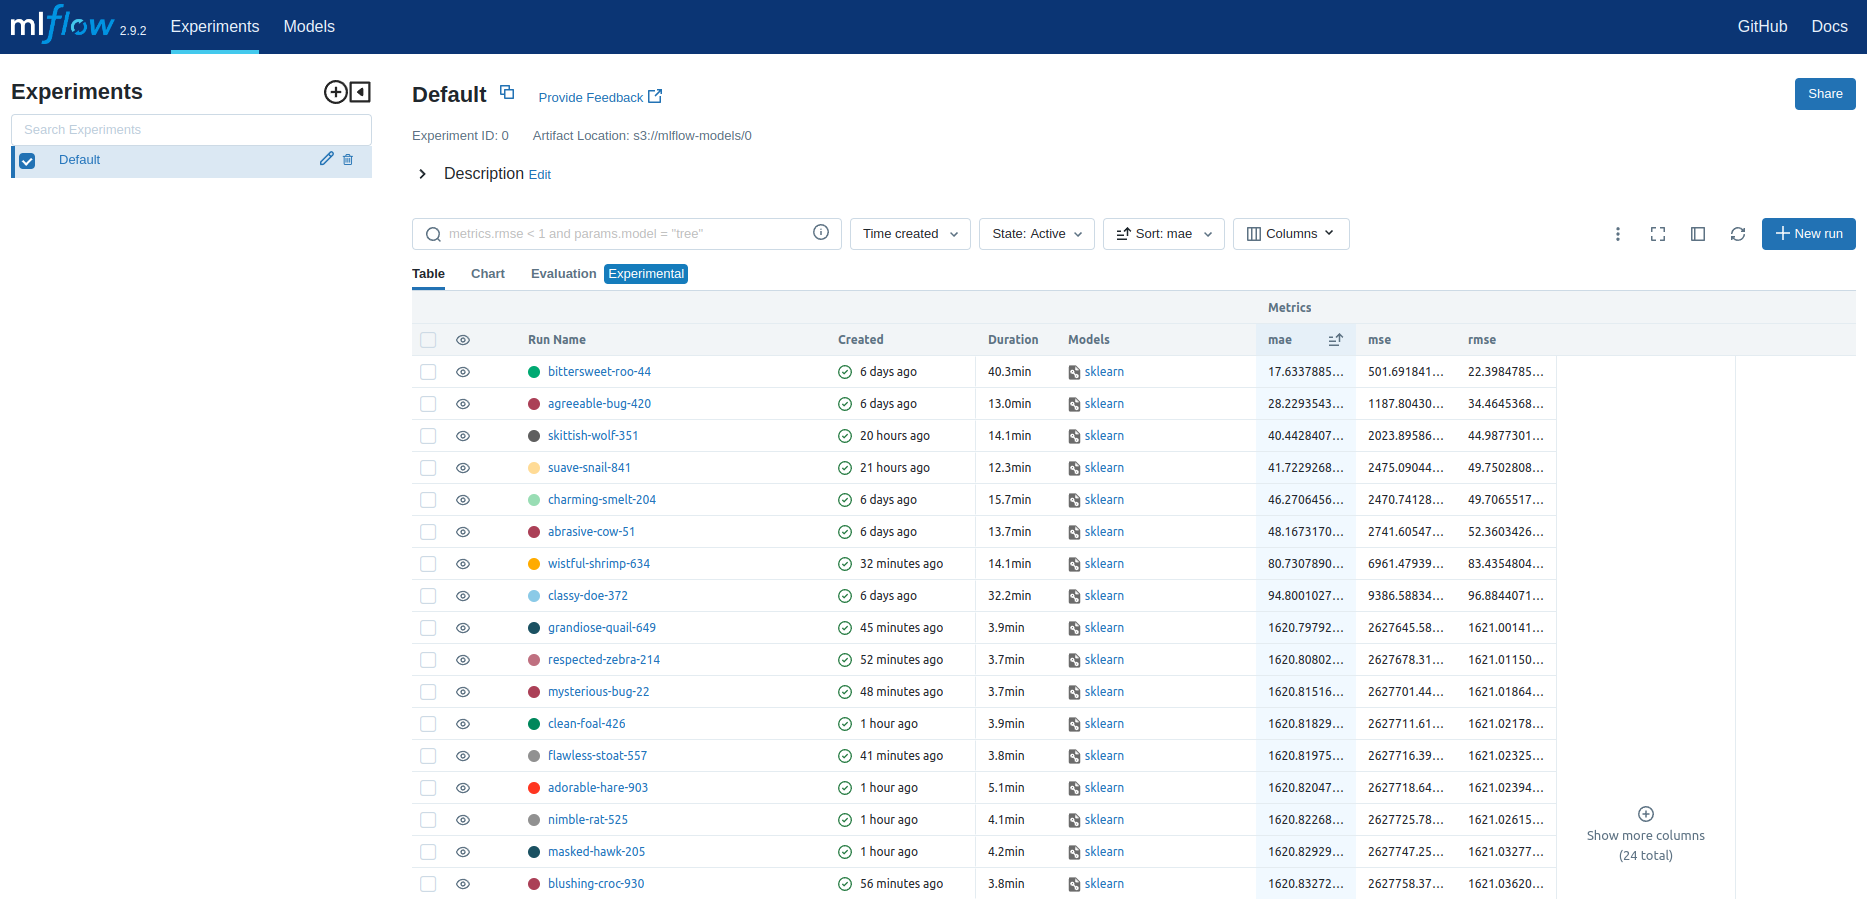
\includegraphics[width=\textwidth]{figures/MLFlow_Model_Overview.png}
    \caption{MlFlow Overview}
    \label{fig:mlflow_overview}
\end{figure}

\begin{figure}[H]
    \centering
    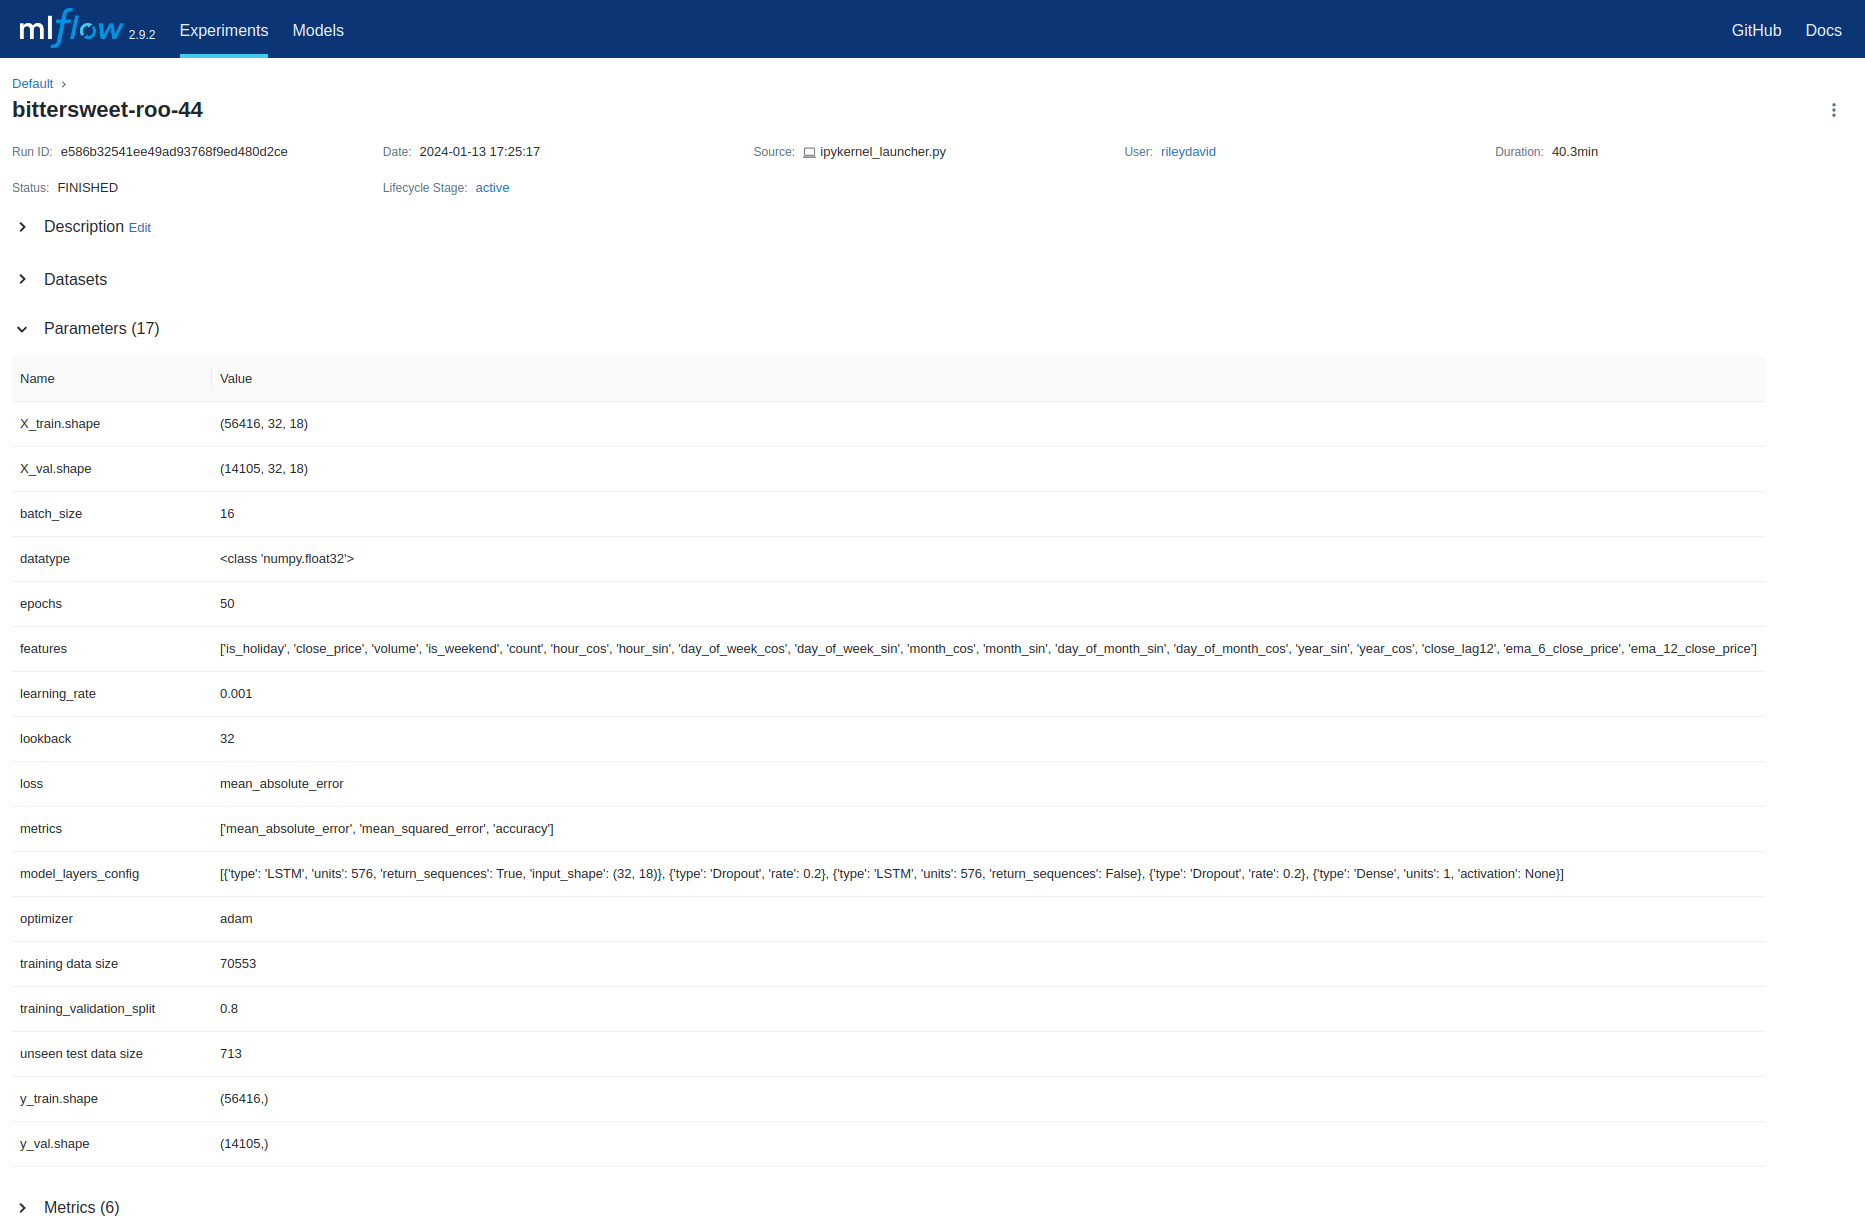
\includegraphics[width=0.93\textwidth]{figures/MlFlow_Model_parameters.png}
    \caption{MlFlow Parameter Tracking}
    \label{fig:mlflow_parameter}
\end{figure}

This provides the user with an overview of the metrics (Figure \ref{fig:mlflow_metrics}) from an MLflow run. The interface displays the metrics recorded for a specific model, such as explained variance, mean absolute error (MAE), mean absolute percentage error (MAPE), mean squared error (MSE), R-squared (r2), and root mean squared error (RMSE). These metrics are critical for assessing the model's predictive accuracy and variance explanation capability. The values are neatly tabulated, allowing for quick review and comparison. 

\begin{figure}[H]
    \centering
    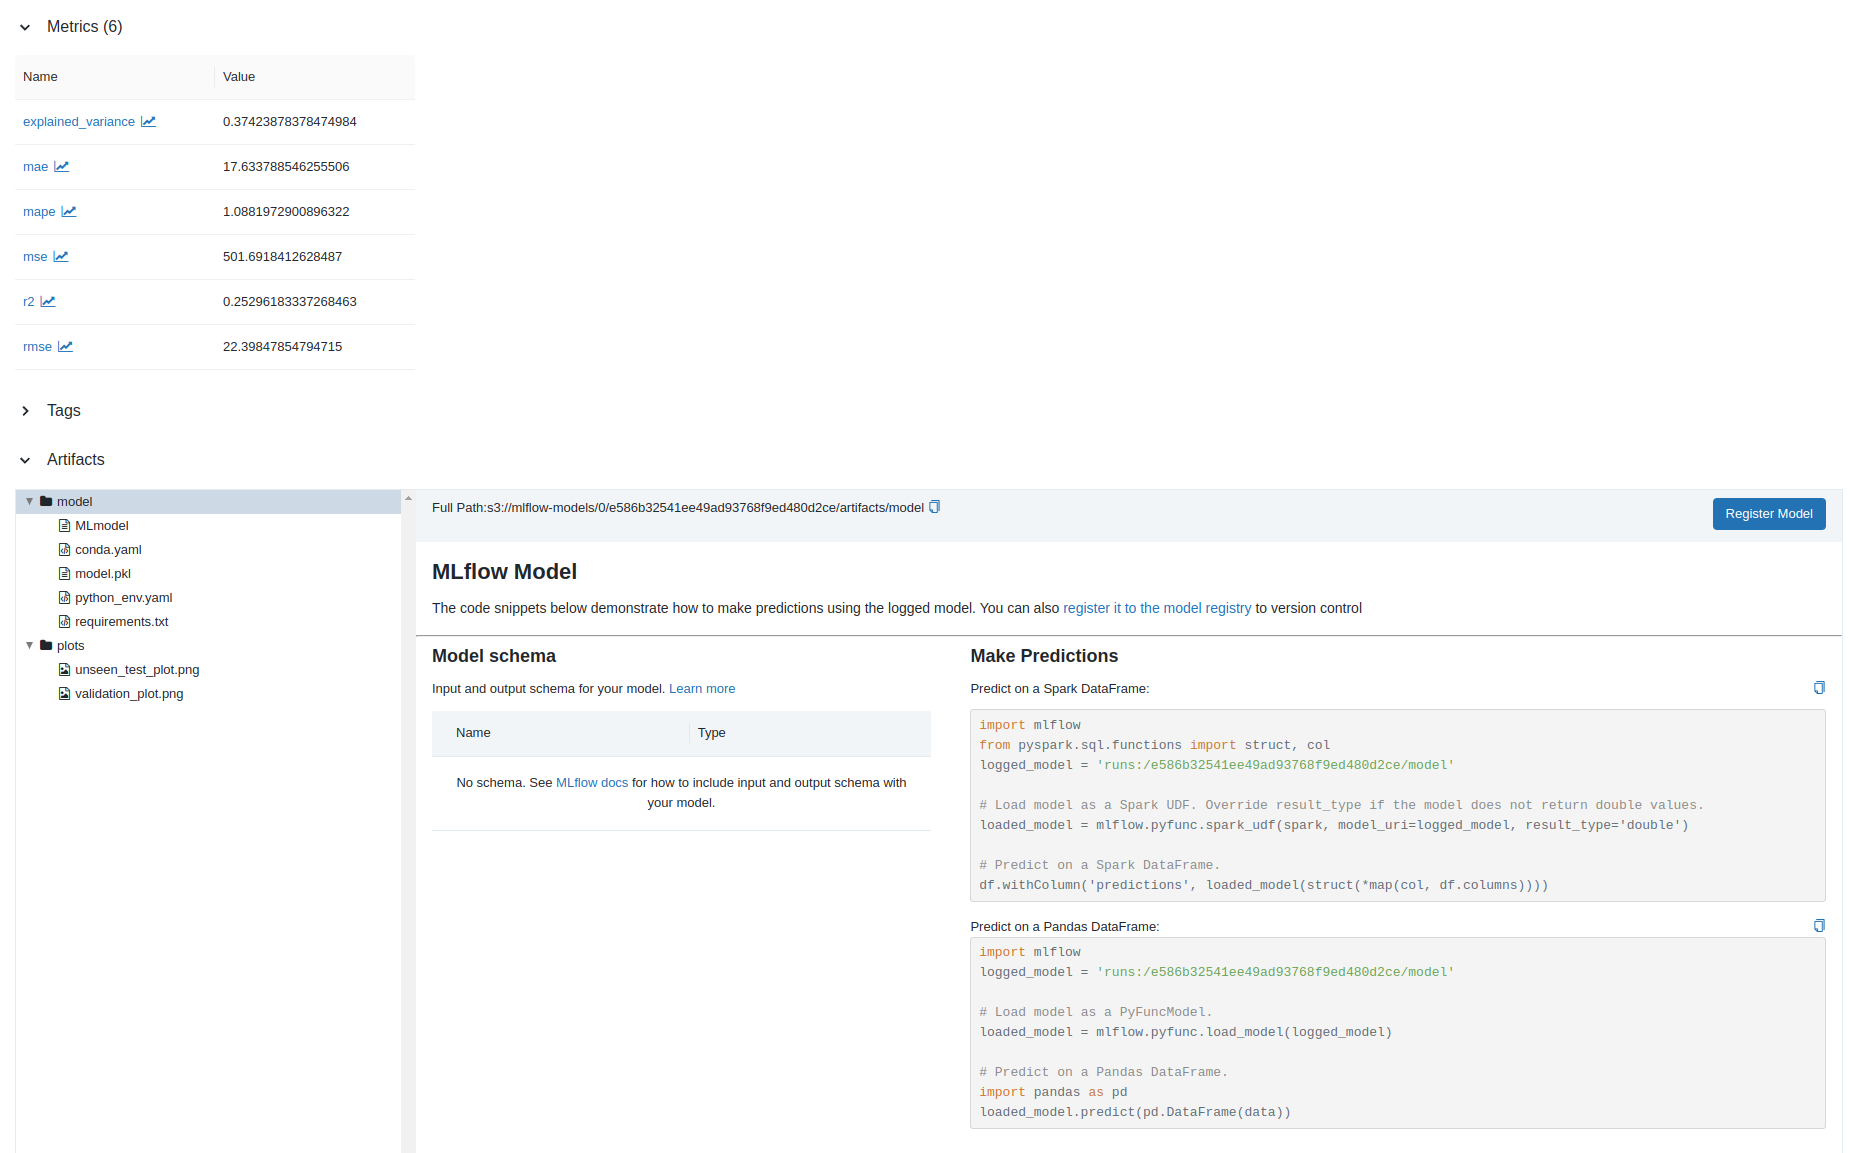
\includegraphics[width=0.93\textwidth]{figures/Mlflow_model_metrics.png}
    \caption{MlFlow Metrics Tracking}
    \label{fig:mlflow_metrics}
\end{figure}

Overall the model tuning process already presents a robust foundation for exploring hyperparameters, but to further enhance this exploration, integrating diverse LSTM architectures could provide a significant leap in model sophistication. This approach not only would broaden the experimental scope but also aligns with the initial strategy of implementing a customizable LSTM model, which has proven instrumental in simplifying the documentation and understanding of the model's structure. Further expansion into varied LSTM designs could unveil new insights and performance benchmarks in the models predictive capabilities.

\section{Model Evaluation}
\label{section:model_evaluation}
The models have been evaluated on the unseen test dataset (Section \ref{section:splitting_dataset}), which is made up of 327 time steps.

\subsection{Metrics}
The top two models have been evaluated using the following metrics:
\begin{itemize}
    \item \textbf{Explained variance (EV):} A measure of how well the model explains the variance in the target variable. A higher EV value indicates that the model is able to capture a greater portion of the underlying patterns in the data.
    \item \textbf{Mean absolute error (MAE):} A measure of the average difference between the predicted and actual values of the target variable. The lower the value the more accurate the predictions are. 
    \item \textbf{Mean squared error (MSE):} A measure of the average squared difference between the predicted and actual values of the target variable. A lower MSE value indicates that the model's predictions are closer to the actual values. 
    \item \textbf{Root mean squared error (RMSE):} This metric is the square root of the MSE and provides an indication of the standard deviation of the errors. A lower RMSE value indicates that the model's predictions are more consistent and less spread out. 
    \item \textbf{Mean absolute percentage error (MAPE):} A measure of the average absolute percent error for each prediction compared to the actual values. MAPE expresses the accuracy as a percentage, providing a simple and intuitive understanding of the model's predictive performance. A lower MAPE value indicates that the model's predictions are closer to the actual values in terms of percentage, making it particularly useful for understanding the relative error in cases where the target variable spans a wide range of values.
    \item \textbf{R-squared (\( R^2 \)):} A measure of the proportion of the variance in the target variable that can be attributed to the model. A higher \( R^2 \) value indicates that the model is able to explain a greater portion of the variance in the data, but it does not necessarily mean the model is good in an absolute sense. \\
\end{itemize}

\subsection{Model 1: amusing-wren-58}
This section provides a detailed evaluation of Model 1 \texttt{amusing-wren-58}, demonstrating its predictive performance through key statistical metrics and a visual comparison of predicted versus actual prices.

\begin{table}[H]
\centering
\begin{tabular}{l l p{10cm}}
\textbf{Metric} & \textbf{Value} & \textbf{Explanation} \\
\hline
EV & 0.838 & The EV score of 0.838 suggests that the model accounts for approximately 83.8\% of the variance in the target variable. This indicates a strong ability of the model to capture the underlying trends and patterns in the data. \\
MAE & 10.64 & The MAE value implies that the model's predictions are, on average, 10.64 units from the actual values. While this shows a degree of accuracy, there is potential for the model to be more precise. \\
MSE & 175.89 & The MSE value signifies that the models errors, when squared, average to this value. Although lower would be better, this indicates a moderately accurate model that may benefit from further refinement. \\
RMSE & 13.26 & The RMSE value reflects the model's prediction consistency. It is a measure of dispersion, showing that the model's errors are generally not too spread out, which suggests a reliable model performance. \\
MAPE & 0.6574 & With a MAPE of 65.74\%, this metric reveals that the model's predictions deviate from the actual values by this percentage on average. This relatively high value points to an area where the model could be improved for better accuracy. \\
\( R^2 \) & 0.821 & The coefficient of determination, or \( R^2 \), is 0.821, indicating that the model effectively captures 82.1\% of the variability in the data. This underscores a strong predictive capability, but it does not necessarily mean the model is good. \\
\end{tabular}
\caption{Model 1 - Metrics and Evaluation (amusing-wren-58)}
\label{table:model_1_evaluation}
\end{table}

The displayed plot (Figure \ref{fig:amusing-wren})  features two lines, where the blue line indicates the actual closing prices, and the orange line represents the predictions made by Model 1: amusing-wren-58. Upon examination, the model's predictions roughly track the actual prices for the most part, reflecting a decent  understanding of the price movement patterns. Both lines exhibit similar trends and volatilities, indicating that the model has a grasp of the temporal dynamics of the price data. \\

\begin{figure}[H]
    \centering
    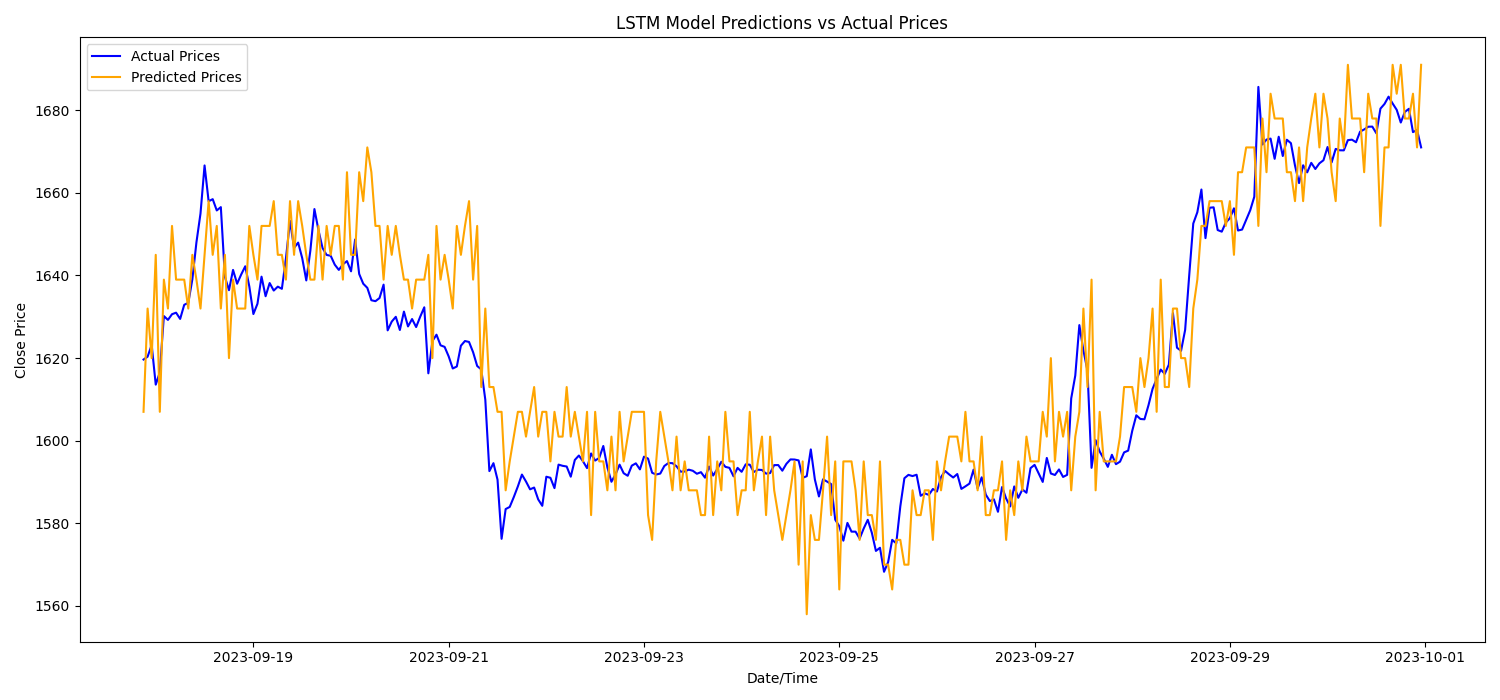
\includegraphics[width=\textwidth]{figures/amusing-wren-58.png}
    \caption{Model 1 - Prediction vs Actual Prices (amusing-wren-58)}
    \label{fig:amusing-wren}
\end{figure}

However, there are noticeable instances where the predicted prices do not align with the actual prices, such as during periods of sideways moving markets, for example in the time period between 2023-09-21 and 2023-09-25, but it does seem to catch rapid peaks quite well between 2023-09-27 and 2023-09-29. These discrepancies might be attributed to the model's limitations in capturing sudden market shifts or anomalies. Despite this, the overall alignment of the two lines throughout the plot signals a decent predictive performance, corroborated by the model's high explained variance score and the tight clustering indicated by the mean absolute error and root mean squared error metrics. The R-squared value of 0.821 further substantiates the model's ability to accurately reflect the majority of the variability in the closing prices, but there is definitely the need for refinement as the model seems to be very sensitive and easily swings far beyond the true values during relatively stable periods. 
\clearpage
\subsection{Model 2: clean-mare-368}
The model 2 \texttt{clean-mare-368} achieved the following scores: 

\begin{table}[H]
\centering
\begin{tabular}{l l p{10cm}}
\textbf{Metric} & \textbf{Value} & \textbf{Explanation} \\
\hline
EV & 0.897 & The EV of 0.897 suggests that the model explains approximately 89.7\% of the variance in the target variable, which indicates the model is capturing most of the variability in the data. \\
MAE & 8.74 & The MAE value suggests that, on average, the model's predictions are approximately 8.74 units away from the actual price. Given the scale of the price, this seems to be a reasonably low error, indicating the model's predictions are fairly accurate. \\
MSE & 121.07 & The MSE value is a measure that squares the errors, penalizing larger errors more severely. This value being relatively low is indicative of the model not making a lot of large errors when inferring the close price. \\
RMSE & 11.00 & The RMSE value indicates that the model's predictions are consistent and less spread out, emphasizing its improved accuracy and reliability compared to Model 1. \\
MAPE & 0.540 &  A MAPE of 0.540, or 54.0\%, is still relatively high even though the other metrics have improved compared to Model 1. This might indicate that while the model performs well in general, it may have periods where its predictions are off by a larger percentage, which could pose a weak point. \\
\( R^2 \) & 0.877 & The \( R^2 \) value is strong, indicating that the model does a good job of fitting the data and can explain a large proportion of the variance. \\
\end{tabular}
\caption{Model 2 - Metrics and Evaluation for Cryptocurrency Price Prediction}
\label{table:new_model_evaluation}
\end{table}

From the graph (Figure: \ref{fig:clean-mare}) and the metrics (Table: \ref{table:new_model_evaluation}) provided, it can be infered that the model's strength lies in its ability to capture the general trend of the actual closing prices, as indicated by the high EV and R-squared values. It also makes predictions that are, on average, quite close to the actual values (low MAE and RMSE). However, the graph shows that at certain points, particularly around the peaks and troughs, the model predictions diverge from the actual prices. This could be due to the model not capturing some of the more volatile movements in the price data, which could be considered a weak point. The high MAPE value suggests that there are instances where the percentage error is quite large, which might occur during these volatile periods, indicating a potential area for improvement in model performance. 

\begin{figure}[H]
    \centering
    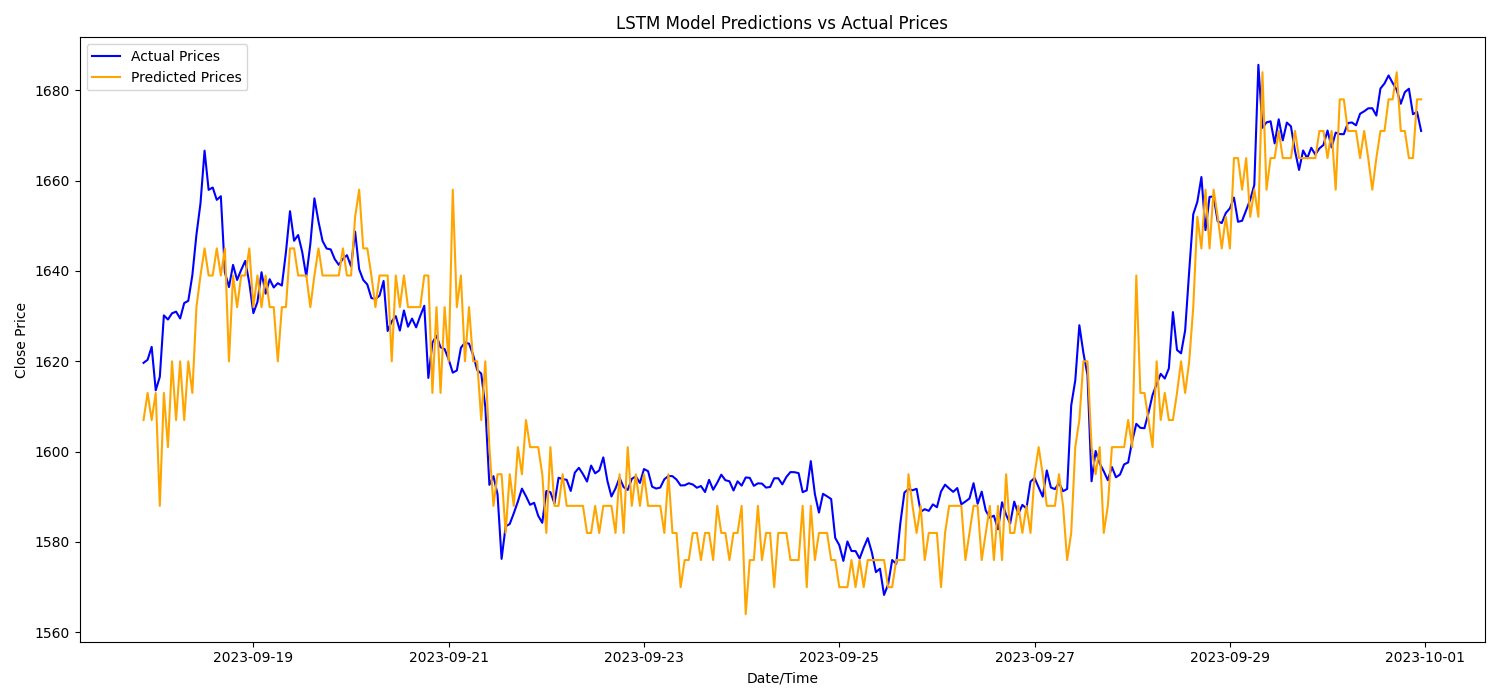
\includegraphics[width=\textwidth]{figures/clean-mare-368.png}
    \caption{Model 2 - Prediction vs Actual Prices (clean-mare-368)}
    \label{fig:clean-mare}
\end{figure}

\subsection{Model Architecture Comparison}
In the following section, the key architectural differences between Model 1 and Model 2 are outlined, which may account for the improved performance in Model 2.

\subsubsection{LSTM Structure}
For Model 1, shown in Listing \ref{lst:model_1_architecture}, the architecture comprises of three LSTM layers, with 228 units each. The first two LSTM layers have the \texttt{return\_sequences} parameter set to True, indicating that they return the full sequence to the next layer. This setup is typical in stacked LSTM configurations where the sequence information should be maintained. The third LSTM layer has \texttt{return\_sequences} set to False, which means it only returns the final output, preparing the data to be fed into the Dense layer. The Dense layer serves as the output layer with a single unit and uses the \texttt{selu} activation function, which is a scaled exponential linear unit that can lead to better convergence during training and seemed to improve the model performance compared to other activation functions (e.g., relu).

\begin{lstlisting}[language=python, caption={Model 1 Structure (amusing-wren-58)}, label={lst:model_1_architecture}]
[{'type':'LSTM', 'units':228, 'return_sequences':True, 'input_shape':(12, 19)},
{'type':'LSTM', 'units':228, 'return_sequences':True},
{'type':'LSTM', 'units':228, 'return_sequences':False},
{'type':'Dense', 'units':1, 'activation':'selu'}]
\end{lstlisting}

Model 2 (Listing \ref{lst:model_2_architecture}) follows a very similar structure but with each LSTM layer containing 240 units, slightly more than Model 1. Additionally, the input shape reflects one additional feature in the data (20 features instead of 19), which could potentially capture more information about the system being modeled. The increased number of units in the LSTM layers may allow Model 2 to learn more complex patterns or relationships in the data, which could be a reason for its improved performance.

\begin{lstlisting}[language=python, caption={Model 2 Structure (clean-mare-368)}, label={lst:model_2_architecture}]
[{'type': 'LSTM', 'units': 240, 'return_sequences': True, 'input_shape': (12, 20)}, 
{'type': 'LSTM', 'units': 240, 'return_sequences': True}, 
{'type': 'LSTM', 'units': 240, 'return_sequences': False}, 
{'type': 'Dense', 'units': 1, 'activation': 'selu'}]
\end{lstlisting}

Both models conclude with a Dense output layer with the same \texttt{selu} activation function, suggesting that the key architectural differences lie in the number of units in the LSTM layers and the dimensionality of the input data.

\subsubsection{Parameters}

The parameters for Model 1 and Model 2 are very similar and both models have been trained on the same dataset. For clarity, the dataset preparation is detailed in Section \ref{section:data_preparation}.

\begin{table}[h!]
\centering
\begin{tabular}{|l|l|}
\hline
\textbf{Parameter} & \textbf{Value} \\
\hline
Learning Rate & 0.001 \\
\hline
Lookback Period & 12 \\
\hline
Metrics & mean\_absolute\_error, mean\_squared\_error, accuracy \\
\hline
Full Dataset Size & 32361 \\
\hline
Training Data Size & 25879 \\
\hline
Validation Set Size & 6470 \\
\hline
Unseen Test Data Size & 327 \\
\hline
Optimizer & Adam \\
\hline
Data Type & numpy.float32 \\
\hline
Batch Size & 16 \\
\hline
\end{tabular}
\caption{Shared Parameters for Model 1 and Model 2}
\label{table:shared_parameters}
\end{table}

The primary difference in parameters between the two models is the set of features used as input data, which are as follows:

\begin{itemize}
    \item Model 1 Features: \{'is\_holiday', 'close\_price', 'volume', 'is\_weekend', 'count', 'hour\_cos', 'hour\_sin', 'day\_of\_week\_cos', 'day\_of\_week\_sin', 'month\_cos', 'month\_sin', 'day\_of\_month\_sin', 'day\_of\_month\_cos', 'year\_normalized', 'close\_lag12', 'close\_lag96', 'ema\_12\_close\_price', 'ema\_48\_close\_price', 'ema\_96\_close\_price'\}
    \item Model 2 Features: \{'is\_holiday', 'close\_price', 'volume', 'is\_weekend', 'count', 'hour\_cos', 'hour\_sin', 'day\_of\_week\_cos', 'day\_of\_week\_sin', 'month\_cos', 'month\_sin', 'day\_of\_month\_sin', 'day\_of\_month\_cos', 'year\_normalized', 'close\_lag12', 'close\_lag96', 'ema\_12\_close\_price', 'ema\_48\_close\_price', 'ema\_96\_close\_price', 'ema\_168\_close\_price'\}
\end{itemize}

The additional feature \texttt{ema\_168\_close\_price} in Model 2 could be a contributing factor to its improved performance. One of the key differences is the loss function used during training. Model 2 uses Mean absolute percentage error as the loss function, which directly optimizes percentage errors, possibly leading to improved performance in metrics that are based on percentages, such as MAPE itself. Model 1 has been trained using the Mean absolute error, which optimizes for absolute differences without considering the relative scale of the target variable, potentially making it less sensitive to proportionally large errors that could be more impactful in a financial context. \\

These differences suggest that Model 2 may be better at capturing both the short- and long-term dependencies in the data due to the additional feature and increased complexity of the LSTM layers and the more ideal loss function.

\subsection{Model Performance Comparison and Conclusion}
Comparing the performance of Model 1: amusing-wren-58 and Model 2: clean-mare-368, several insights can be drawn from their respective metrics and visual analysis. Model 2 demonstrates a notable improvement over Model 1 across several key metrics, highlighting its enhanced predictive capabilities. \\

Model 2's Explained Variance (EV) of 0.897 significantly surpasses Model 1's EV of 0.838, indicating a superior ability to capture the variance in the target variable. This higher EV suggests that Model 2 is more adept at understanding the underlying patterns and trends in the data. \\

The Mean Absolute Error (MAE) further cements Model 2's lead with a value of 8.74, compared to Model 1's MAE of 10.64. This reduction in MAE signifies that Model 2's predictions are closer to the actual values, showcasing its heightened accuracy. \\

In terms of the Mean Squared Error (MSE) and Root Mean Squared Error (RMSE), Model 2 again outperforms Model 1 with lower values of 121.07 and 11.00, respectively. These metrics indicate that Model 2 not only makes fewer large errors but also maintains a consistent level of prediction accuracy across the dataset. \\

However, the Mean Absolute Percentage Error (MAPE) reveals a nuanced perspective. Although the 54.0\% MAPE for Model 2 might appear elevated at first glance, it is essential to not lean on this figure alone and consider all metrics. It does indicate that Model 2 generally delivers reasonable results, yet it encounters challenges in accurately predicting certain cases or outliers, leading to significant discrepancies from the true values. \\

The R-squared value for Model 2 stands at 0.877, an improvement over Model 1's 0.821. This indicates that Model 2 is better at modeling the variance in the data, providing a more accurate representation of the market dynamics. \\

In conclusion, Model 2: clean-mare-368 shows a clear advancement in predictive performance over Model 1: amusing-wren-58, evidenced by its superior metrics across the board. Model 2 demonstrates its enhanced ability to accurately capture and predict the underlying trends within the dataset. While the MAPE suggests room for improvement in handling outliers or specific market conditions, the overall metrics indicate a robust model capable of providing valuable insights. These findings underscore the importance of comprehensive model evaluation, beyond a single metric, to truly understand and appreciate a model's predictive power and potential limitations.
 

\section{Backend}
As the backbone of any robust machine learning system, the backend architecture requires careful consideration of performance, stability, and security. Rust, an emerging systems programming language, offers a compelling combination of features making it an excellent choice for the backend.

\subsection{Rust Libraries for Backend Services}

To build a backend that is both performant and scalable, a suite of Rust libraries have been utilized, each serving a distinct purpose in the backend architecture. The following libraries form the core of the backend:

\begin{itemize}
    \item \textbf{Axum \cite{AxumDocumentation}} Version 0.7.2 of the Axum library is used for crafting web applications. Axum leverages the asynchronous runtime of Tokio and focuses on ergonomics and modularity. 
    \item \textbf{Tokio \cite{TokioDocumentation}} The asynchronous runtime Tokio, version 1.23, provides a non-blocking event loop that drives the application's I/O operations.
    \item \textbf{Serde \cite{SerdeDocumentation}} Serialization and deserialization within the service are handled by Serde, version 1.0, a framework enabling efficient, declarative, and generic data serialization. The "derive" feature is activated, allowing for the automatic generation of code to serialize and deserialize custom data structures.
    \item \textbf{Sqlx \cite{SQLxDocumentation}} The Sqlx library, version 0.7.3, is chosen for database interactions. It provides compile-time checked queries and supports various databases, including PostgreSQL.
\end{itemize}

These libraries form a modern tech stack that bolsters the backend's capacity to handle web services, asynchronous processing, data serialization, and database management efficiently and securely.

\subsection{Collector Module}
\label{section:collector}

The \textbf{Collector Module} serves as the data acquisition gateway of the system. It is implemented to connect with real-time data feeds and extract valuable trade information, thereby feeding the system's analytics and decision-making processes.

\subsubsection{Kraken WebSockets API Overview}
The Kraken WebSockets API \cite{KrakenWebsocketsDocumentation} provides a real-time streaming service for cryptocurrency market data. Through WebSocket connections, clients can subscribe to various data channels to receive immediate updates, a feature that the system takes full advantage of for collecting trade data.

\paragraph{Efficient Data Streaming}
The efficient streaming of live data via the Kraken WebSockets API is instrumental for applications that depend on up-to-the-minute market information, such as algorithmic trading platforms and analytical tools. By leveraging this API, the backend system, is able to collect, process, and utilize market data in a way that aligns with the high-throughput and low-latency requirements of modern trading systems.

\paragraph{Trade Subscription}
Subscribing to trade data is a key feature of the API. The trade subscription (Listing \ref{lst:trade_sub}) provides a live feed of trade executions on the exchange, including details such as price, volume, and time. The payload structure for trade messages (Listing \ref{lst:trade_payload}) consists of multiple fields (price, volume, time, side, order type, misc), ensuring that clients have access to comprehensive trade data for their selected currency pairs.


\begin{lstlisting}[language=bash, caption={Subscription for Trade Data}, label={lst:trade_sub}]
{
  "event": "subscribe",
  "pair": [
    "XBT/USD"
  ],
  "subscription": {
    "name": "trade"
  }
}
\end{lstlisting}

\begin{lstlisting}[language=bash, caption={Trade Message Payload}, label={lst:trade_payload}]
[
  0,
  [
    [
      "5541.20000",
      "0.15850568",
      "1534614057.321597",
      "s",
      "l",
      ""
    ],
    [
      "6060.00000",
      "0.02455000",
      "1534614057.324998",
      "b",
      "l",
      ""
    ]
  ],
  "trade",
  "XBT/USD"
]
\end{lstlisting}

\subsubsection{Functionality and Workflow}
The collector initiates a WebSocket connection to the Kraken exchange, subscribing to trade data (Listing \ref{lst:trade_sub}) streams for various cryptocurrency pairs. It maintains a mapping of currency symbols to their corresponding database identifiers, ensuring that incoming trade data can be accurately categorized and stored. \\

Upon receiving a new trade message, the collector performs several critical operations:
\begin{itemize}
    \item Parses the message and filters out non-trade related information such as heartbeats and subscription acknowledgments.
    \item Inserts new trading symbols into the database if they do not exist already, expanding the system's ability to track a broader range of currency pairs.
    \item Converts trade data into internal models and persists them into the database using the trade repository's insertion functionality.
\end{itemize}

The collector's loop continues to listen for new subscription messages and trade data, maintaining an up-to-date and comprehensive dataset for the system.

\paragraph{Asynchronous and Parallel Processing}
The collector is built to leverage Rust's asynchronous runtime and parallel processing capabilities, allowing it to handle high volumes of data with minimal latency. It uses the \texttt{tokio} and \texttt{rayon} libraries to perform non-blocking data operations and parallel computations.

\paragraph{Error Handling and Logging}
Robust error handling is embedded within the collector, ensuring that any issues encountered during data collection or insertion are logged and managed appropriately. This proactive approach to monitoring ensures the system's reliability and data integrity.

In essence, the trade data collector serves as a resilient and efficient backend module, tasked with the continuous collection of trade data, which forms the backbone of the system's data-driven analytics and machine learning capabilities.

\subsection{Webserver}
The backend webserver exhibits a modular design that significantly enhances the system's flexibility and maintainability. This is achieved by splitting the applications into distinct components, where each component is responsible for a specific aspect of the system's functionality.

\begin{itemize}
\item \textbf{Server Module}: Acts as the entry point of the application, handling server initialization and configuration (Listing \ref{lst:webserver_main}).
\begin{lstlisting}[language=rust, caption={Webserver Main}, label=lst:webserver_main]
#[tokio::main(flavor = "multi_thread", worker_threads = 6)]
async fn main() -> Result<(), ()> {
    dotenv().ok();
    logger::run().await;
    info!("server is starting up ...");

    let (sender, receiver) = mpsc::channel(1);

    collector::collector::run(receiver).await;
    webserver::webserver::run(sender).await;
    Ok(())
}
\end{lstlisting}

\item The \textbf{Webserver Module} is architected to set up the web routing and middleware configurations that dictate the processing of HTTP requests and generation of responses. This module uses the Axum framework, renowned for its ergonomic design and powerful features, to define clear and concise routes for different endpoints. Each route is associated with a specific handler function that executes when the route is accessed.

Middleware components are strategically placed to manage cross-cutting concerns that apply across multiple routes. These concerns include but are not limited to logging for monitoring and debugging, authentication to secure endpoints, and error handling to gracefully manage any unexpected conditions during request processing.

The module is designed with modularity at its core, with routes organized into distinct sub-modules, which enhances the clarity and scalability of the codebase, allowing for independent development and testing of different API endpoints. A CORS layer has been incorporated to ensure that the server can interact with web clients from different origins, making it versatile and web-friendly.

Below is the setup code for the Axum webserver, detailing the initialization process, and the middleware and routes configuration:

\begin{lstlisting}[language=rust, caption={Webserver Axum Setup with Annotations}, label=lst:axum_webserver_init]
pub async fn run(sender: tokio::sync::mpsc::Sender<String>) {
    // Initialize database connection and application state.
    let pool = postgresdb::get_connection().await; 
    let app_state = AppState::new(pool.clone(), /* Redis cache */ None, sender);

    // Configure CORS to allow interactions from any origin.
    let cors = CorsLayer::new()
        .allow_methods(Any)
        .allow_origin(Any)
        .allow_headers(Any);

    // Define the router and its associated routes.
    let app = Router::new()
        .route("/ping", get(ping))
        .merge(routes::ohlc::routes::router(pool).await) 
        .merge(routes::symbol::routes::router(app_state).await) 
        .merge(routes::import::routes::router(pool).await) 
        .merge(routes::modelexecution::routes::router(pool).await) 
        .merge(routes::trade::routes::router(pool).await) 
        .merge(routes::upload::routes::router().await) 
        .layer(cors); // Apply CORS settings to all routes

    // Determine server address and start listening for requests.
    let address = SocketAddr::from(get_address().await);
    let listener = TcpListener::bind(address).await.unwrap();
    axum::serve(listener, app.into_make_service())
        .await
        .unwrap_or_else(|_| panic!("Server cannot launch."));
}
\end{lstlisting}

\item The \textbf{Service Module} within the system architecture encapsulates specialized sub-modules, each dedicated to a distinct set of data management and operational tasks:

\begin{itemize}
    \item \textbf{Import Sub-Module}: Oversees the importation process of historical data, ensuring the database can be populated with historical datasets and materialized views are refreshed to account for the newly imported data.
    \item \textbf{Symbol Sub-Module}: Manages the retrieval and management of symbol data, interfacing directly with the \texttt{symbol\_repository} to ensure up-to-date symbol information is available.
    \item \textbf{Trade Sub-Module}: Handles the acquisition of live trade data, utilizing the \texttt{trade\_repository} to fetch and process trade transactions from the market.
    \item \textbf{OHLC Sub-Module}: Deals with the retrieval of Open-High-Low-Close (OHLC) data, critical for market analysis, by making use of the \texttt{ohlc\_repository}.
    \item \textbf{Model Execution Sub-Module}: Orchestrates the execution of machine learning models, coordinating the loading of model configurations and relevant data from Timescale. It facilitates model execution requests to the model service, which ultimately yield predictive outcomes such as the estimated close\_price.
\end{itemize}

Each submodule within the service module is linked to a specific domain, ensuring the separation of concerns and efficient data handling that is crucial for the system's responsiveness and analytical capabilities. \\

The following code snippet showcases an example of the \texttt{symbol\_service}. This service is responsible for retrieving symbol data from the repository and transforming it into a data transfer object (DTO) format that is optimized for client-side consumption.

\begin{lstlisting}[language=rust, caption={Symbol Service Fetch Function}, label=lst:symbol_service]
pub async fn get_symbols(pool: &sqlx::PgPool) -> Result<Vec<SymbolDto>, GenericError> {
    match symbol_repository::get_symbols(pool).await {
        Ok(data) => {
            let result: Vec<SymbolDto> = data
                .into_par_iter()
                .map(|model| SymbolDto::from(&model))
                .collect();

            Ok(result)
        }
        Err(err) => {
            Err(err)
        },
    }
}
\end{lstlisting}

This function demonstrates a typical service operation, where data is fetched from the repository and transformed. The use of parallel iteration through \texttt{into\_par\_iter} signifies the system's commitment to performance and efficiency.

\item \textbf{Repository Module}: Encapsulates all database interactions, abstracting the complexity of data queries and manipulations. It is further divided into sub-modules for different domain entities like symbols (Listing \ref{lst:symbol_repository}), trades, and OHLC data, promoting a single responsibility principle.
\begin{lstlisting}[language=rust, caption={Symbol Repository Example}, label=lst:symbol_repository]
const QUERY_SELECT_SYMBOLS: &str = "SELECT * FROM symbol;";

pub async fn get_symbols(
    pool: &sqlx::PgPool,
) -> Result<Vec<SymbolModel>, GenericError> {
  match sqlx::query(QUERY_SELECT_SYMBOLS)
      .map(|row: PgRow| SymbolModel::from(row))
      .fetch_all(pool)
      .await
  {
      Ok(data) => Ok(data),
      Err(err) => Err(RepositoryError::general_error(err.to_string())),
  }
}
\end{lstlisting}

\item The \textbf{Utils Module} offers a suite of utility functions and shared libraries that facilitate cross-application use, significantly increasing code reusability. For instance, Listing \ref{lst:webserver_address_util} showcases a utility function that retrieves the address configuration for the webserver. While this function is currently tailored for the webserver, it can be refactored to generically obtain host IP addresses and ports for various services by reading from the environment configuration. Such a modification would enhance the module's reusability across different components of the application.
\begin{lstlisting}[language=rust, caption={Util get\_address for Webserver}, label=lst:webserver_address_util]
pub async fn get_address() -> (IpAddr, u16) {
    let host_ip_address =
        std::env::var("WEBSERVER_IP").unwrap_or_else(|_| panic!("WEBSERVER_IP must be set!"));
    let host_port =
        std::env::var("WEBSERVER_PORT").unwrap_or_else(|_| panic!("WEBSERVER_PORT must be set!"));

    let ip_address = host_ip_address
        .parse::<IpAddr>()
        .expect("IP Adress invalid");
    let port = host_port.parse::<u16>().expect("PORT is invalid.");

    let url_message = format!(
        "executed: initializing server url = {}:{}",
        &ip_address, &port
    );
    info!(url_message);

    (ip_address, port)
}
\end{lstlisting}


\end{itemize}

\paragraph{Separation of Concerns}
This modular setup is grounded in the separation of concerns principle, which dictates that each module should address a separate piece of the application's functionality. By adhering to this principle, the application not only becomes more manageable and easier to understand but also enhances each module's reusability and testability. \\

The modular nature of this setup makes the webserver highly flexible, allowing for the addition or modification of routes and middleware without disrupting existing functionality. It embodies a cleanly separated architecture that simplifies concern isolation, ultimately leading to a system that is easier to extend, maintain, and troubleshoot.

\subsubsection{Error Handling}
A robust error handling system is vital for maintaining the reliability and predictability of any application. In the provided setup, the system uses a combination of a trait, a struct, and an enumeration to structure and manage errors effectively.

\paragraph{GenericErrorTrait}
The \texttt{GenericErrorTrait} (Listing \ref{lst:generic_error_trait}) is a Rust trait that defines a common interface for error handling. Traits in Rust are similar to interfaces in other languages, providing a way to define shared behavior. This trait includes two methods:
\begin{itemize}
    \item \texttt{get\_message()}: Returns a human-readable error message.
    \item \texttt{get\_code()}: Provides a specific error code, useful for categorizing and responding to different error types.
\end{itemize}

\begin{lstlisting}[language=rust, caption={GenericErrorTrait Utils Module}, label=lst:generic_error_trait]
pub trait GenericErrorTrait {
    fn get_message(&self) -> String;
    fn get_code(&self) -> String;
}
\end{lstlisting}

\paragraph{ErrorBody Struct}
The \texttt{ErrorBody} struct (Listing \ref{lst:error_body}) is a concrete representation of an error, containing a message and a code. It implements the \texttt{GenericErrorTrait}, thereby adhering to the interface defined by the trait. 
\begin{lstlisting}[language=rust, caption={ErrorBody Utils Module}, label=lst:error_body]
#[derive(Debug)]
pub struct ErrorBody {
    message: String,
    code: String,
}
\end{lstlisting}

\paragraph{GenericError Enum}
The \texttt{GenericError} (Listing \ref{lst:generic_error}) enumeration is a versatile way to encapsulate different error types while maintaining a uniform interface. It has variants for different error contexts, such as \texttt{Repository}, \texttt{Service}, and \texttt{Web}. Each variant holds an \texttt{ErrorBody}, ensuring that every error within the system has a consistent structure.

\begin{lstlisting}[language=rust, caption={GenericError Utils Module}, label={lst:generic_error}]
#[derive(Debug)]
pub enum GenericError {
    Repository(ErrorBody),
    Service(ErrorBody),
    Web(ErrorBody),
}
\end{lstlisting}
\mbox{}\\
This setup offers several advantages:
\begin{itemize}
    \item \textbf{Consistency}: By using a common trait and struct, the system ensures that all errors, regardless of where they occur, have a consistent representation.
    \item \textbf{Flexibility}: The \texttt{GenericError} enum can be easily extended to include more error types as the system evolves.
    \item \textbf{Ease of Use}: The trait and struct provide straightforward methods for creating and handling errors, making the code more readable and maintainable.
    \item \textbf{Error Propagation}: This setup simplifies error propagation across different layers of the application, such as from the repository layer to the web layer.
\end{itemize}

In summary, this error handling system offers a structured and effective approach to managing errors, which is crucial for maintaining the robustness and user-friendliness of the application.

\subsubsection{Environment Configuration}
Employing an environment configuration file is essential for a system that prioritizes security, maintainability, and scalability, ensuring that it remains robust and flexible across various deployment environments. In this case the environment variables have been defined in the docker compose file, which itself makes use of a global \texttt{config.env} file (Section \ref{docker_config_env}) that initializes the environment variables for the backend.


\section{Model Service}

The \textbf{Model Service} operates as a specialized web server within the infrastructure, dedicated to managing the execution of machine learning models. This service plays a pivotal role, closing the gap between the raw data inputs and the derived actionable insights.

\subsection{Operational Workflow}
At its core, the Model Service's primary role involves processing incoming requests that carry both the model configuration (Listing \ref{lst:model_configuration}) and the required data for model inference. Specifically, these requests encompass OHLC (open, high, low, close price) data, volume, and trade count, which are essential for the model inference.

\begin{lstlisting}[language=bash, caption={Model Configuration (JSON)}, label={lst:model_configuration}]
{
  "symbol_id": 1,
  "modelname": "model.pkl",
  "data_type": "np.float32",
  "lookback": 16,
  "lags": [12, 168],
  "window_sizes": [],
  "span_sizes": [6, 12],
  "active": true,
  "features": [
    "is_holiday",
    "close_price",
    "volume",
    "is_weekend",
    "count",
    "hour_cos",
    "hour_sin",
    "day_of_week_cos",
    "day_of_week_sin",
    "month_cos",
    "month_sin",
    "day_of_month_sin",
    "day_of_month_cos",
    "year_normalized",
    "close_lag12",
    "close_lag168",
    "ema_6_close_price",
    "ema_12_close_price"
  ]
}
\end{lstlisting}

The service operates using a singular endpoint, \texttt{/execute}, designed to handle POST requests (Listing \ref{lst:model_service_entry}). Upon receiving a request, the service unpacks the JSON payload, which encapsulates both the model configuration and the necessary data. This configuration delineates all necessary details for the model execution, encompassing the model's name, the input features, parameters, and the comprehensive dataset required for the process. \\

\begin{lstlisting}[language=Python, caption={Model Service Flask Entry Point}, label={lst:model_service_entry}]
from flask import Flask, request, jsonify
from model_execution import * 

app = Flask(__name__)

@app.route('/execute', methods=['POST'])
def execute_model():
    try:
        config = request.json
        model_execution = ModelExecution(config)
        timestamp, price = model_execution.execute()
        return jsonify({"bucket": timestamp, "close_price": price.item()}), 200
    except Exception as e:
        return jsonify({"error": str(e)}), 500

if __name__ == '__main__':
    app.run(debug=False, host='0.0.0.0', port=7000, load_dotenv=True)
\end{lstlisting}

\subsubsection{Model Execution Class}
The initialization of the \texttt{ModelExecution} class (Listing \ref{lst:model_execution_class}) triggers the loading of environment variables via \texttt{load\_dotenv}. These variables play a crucial role in initializing the \texttt{ModelProvider} class. This class bears the responsibility of fetching the machine learning model from an S3-compatible storage solution, specifically MinIO in this context. \\

Upon receiving a request, the \texttt{ModelExecution} class is initialized using the model configuration. This class undertakes the task of transforming the dataset (as detailed in Section \ref{section:data_preparation}), ensuring the inclusion of features as specified in the model configuration. Subsequently, it retrieves the actual model from MinIO (as elaborated in Section \ref{section:minio}). After the model inference, the service compiles a JSON response. This response encapsulates the model's prediction, integrating the relevant timestamp, and providing the inferred close prices.

\begin{lstlisting}[language=Python, caption={Model Execution Class}, label={lst:model_execution_class}]
class ModelExecution:
  def __init__(self, config):
    print("Initializing Model Execution")
    load_dotenv()
    self.config = config

    self.model_provider = ModelProvider(os.getenv('S3_BUCKET'),
                                       config['modelname'],
                                       os.getenv('AWS_ACCESS_KEY_ID'),
                                       os.getenv('AWS_SECRET_ACCESS_KEY'),
                                       os.getenv('S3_ENDPOINT_URL'))

    self.data_service = DataService(os.getenv('BACKEND_ENDPOINT'))

  def execute(self):
    print("Starting execution")
        
    df = pd.DataFrame(self.config['data'])
    df.reset_index(inplace=True)

    data_preperation_service = DataPreparation(df, self.config)

    X = data_preperation_service.prediction_sequence
    X_reshaped = X.reshape(1, int(self.config['lookback']), len(self.config['features']))

    self.model_provider.fetch_model(self.config['modelname'])
    with open(self.config['modelname'], 'rb') as file:
        model = cloudpickle.load(file)

    predicted_price_log = model.predict(X_reshaped, verbose=0)
    predicted_price = np.expm1(predicted_price_log)[0, 0]
        
    parsed_date = datetime.strptime(self.config['from_date'], '%Y-%m-%dT%H:%M:%S%z')
    new_date = parsed_date + timedelta(hours=1)
    output_date = new_date.strftime('%Y-%m-%dT%H:%M:%S') + 'Z'
    print(output_date)
        
    return output_date, predicted_price
\end{lstlisting}

Additionally, the \texttt{DataService} comes into play for interfacing with the backend service for any extra data requirements. Although this class was previously utilized, enhancements have been made to streamline the data flow and minimize execution times by transmitting the required data alongside the initial requests.

The \texttt{ModelExecution} class is at the core of the Model Service, steering the complete lifecycle of executing a machine learning model.

\subsubsection{Significance in the System}
The \texttt{Model Service} is the cornerstone of the system, pivotal for harnessing the power of machine learning in forecasting. By meticulously managing the complexities of model retrieval, data processing, and prediction it ensures that the system delivers precise and timely forecasts, a critical capability in dynamic sectors such as the financial markets.

\section{Frontend}

The frontend of the system is engineered using Angular 17 \cite{AngularOverview} and Node.js \cite{NodejsWebsite}. This combination offers a potent platform for crafting dynamic, responsive, and user-friendly web applications.

\subsection{Dashboard Overview}

The dashboard (Figure \ref{fig:frontend_dashboard}) is a crucial component of the frontend, designed to offer users a comprehensive overview of the system's analytics. It is the focal point for data visualization, presenting both historical and predictive data in an intuitive and accessible manner.
\begin{figure}[ht!]
    \centering
    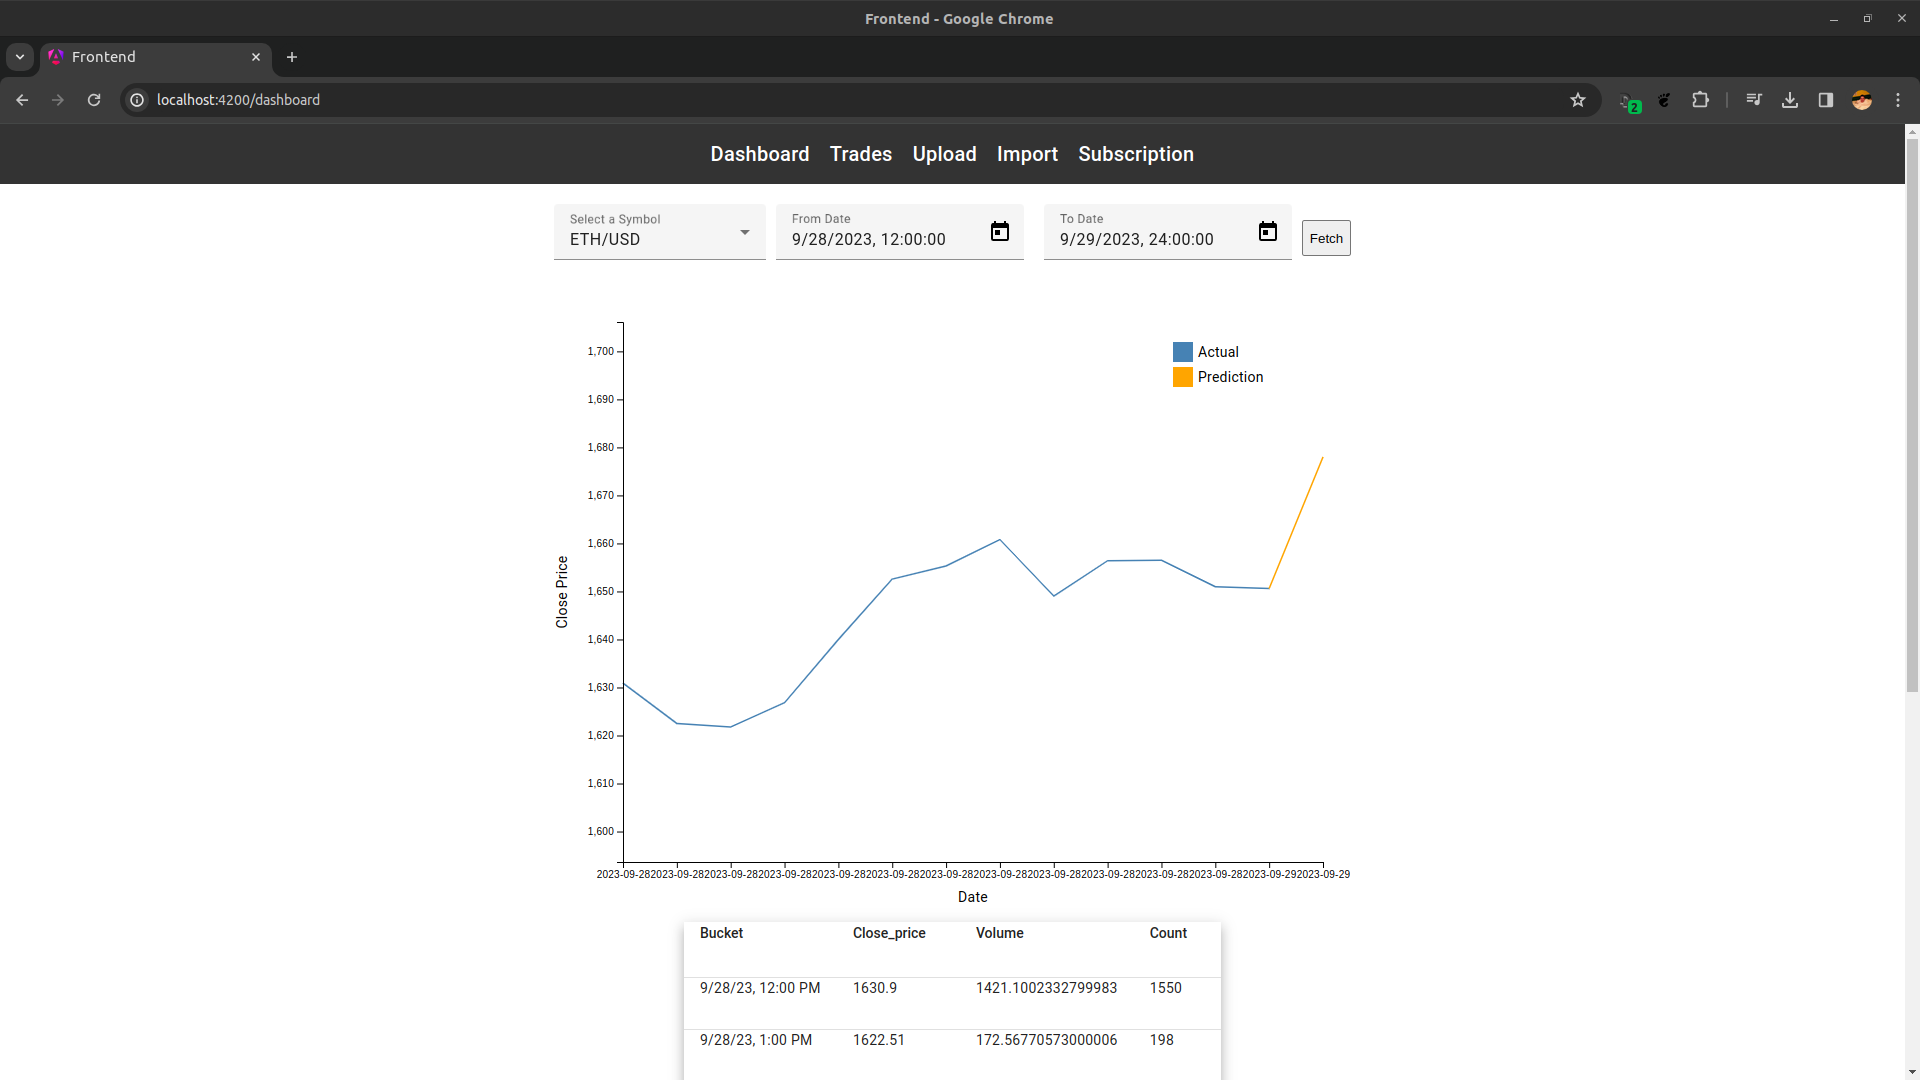
\includegraphics[width=\textwidth]{figures/frontend_dashboard.png}
    \caption{Dashboard}
    \label{fig:frontend_dashboard}
\end{figure}

\subsubsection{User Interface}
The dashboard interface is structured to provide a seamless user experience:
\begin{itemize}
    \item \textbf{Symbol Selection}: Users can choose from a dropdown menu to select different symbols (currency pairs) for which they wish to view a forecast and OHLC data.
    \item \textbf{Date Range}: The dashboard includes a date range picker, allowing users to specify the time frames, they want to analyze.
    \item \textbf{Fetch Data}: The \texttt{Fetch} button initiates the retrieval of data based on the selected symbol and date range, updating the visualizations accordingly.
\end{itemize}

\subsubsection{Data Visualization}
The core of the dashboard is its data visualization:
\begin{itemize}
    \item \textbf{Price Chart}: A line chart prominently displays the close price trends over the selected time period. This chart helps users quickly grasp market movements and identify trends.
    \item \textbf{Prediction Indicator}: Predictive analytics are highlighted on the chart with a distinct color, differentiating predicted values from actual historical data.
\end{itemize}

\subsubsection{Data Table}
Below the chart is a data table that enumerates detailed information:
\begin{itemize}
    \item \textbf{Bucket}: Specific time intervals (e.g., hourly buckets) corresponding to the data points on the chart.
    \item \textbf{Close Price}: Closing price of the asset for each bucket, providing granular insight into price fluctuations.
    \item \textbf{Volume}: Trading volume within each bucket, offering an indication of market activity.
    \item \textbf{Count}: Number of trades that occurred, which can serve as a proxy for market liquidity or activity during the bucket's period.
\end{itemize}


In summary, the frontend dashboard provides a rich, interactive platform for monitoring and analyzing market data. Its intuitive design and visualization make it an essential part of the user interface, enabling effective display and examination of financial data and model predictions.

\subsection{Trades}

The \texttt{Trades} tab (Figure \ref{fig:frontend_trades}) within the frontend is a detailed ledger that presents users with a transaction-level view of trading activity. It complements the aggregate data visualized on the dashboard by providing the granular details of each trade.

\begin{figure}[ht!]
    \centering
    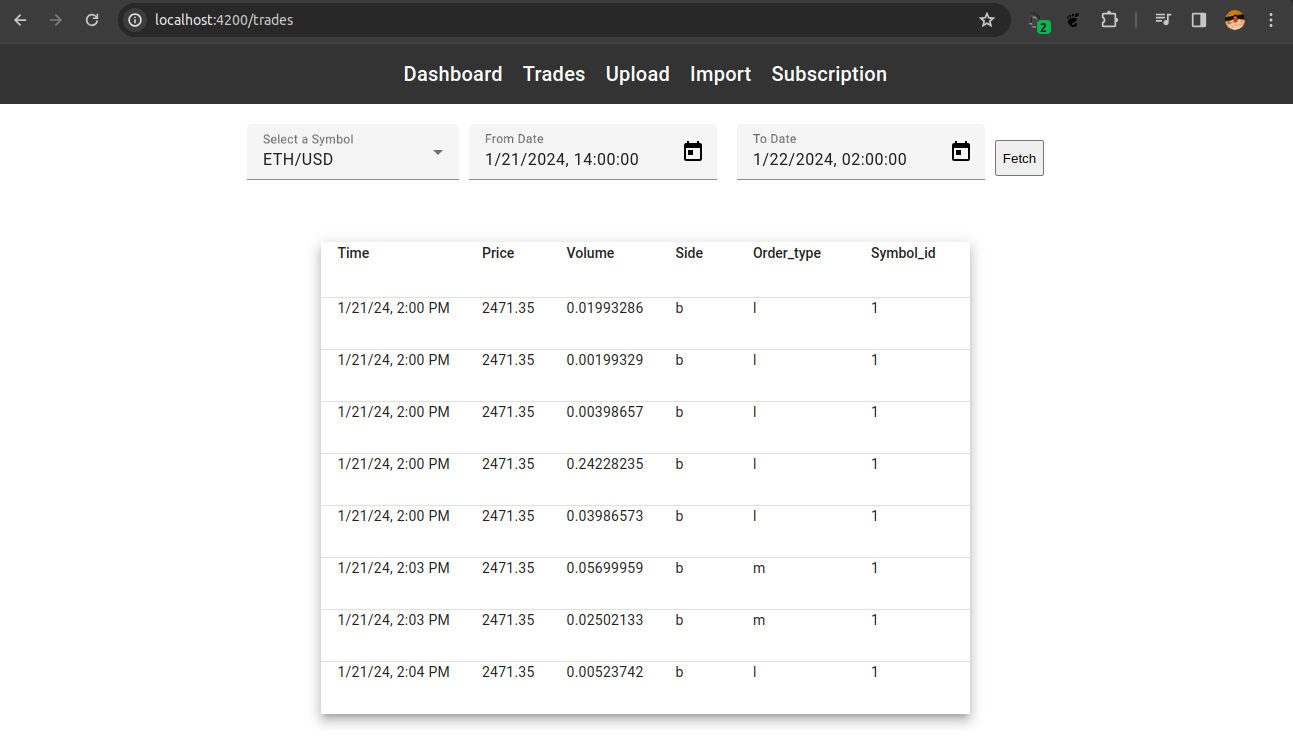
\includegraphics[width=\textwidth]{figures/frontend_trades.png}
    \caption{Trades}
    \label{fig:frontend_trades}
\end{figure}

\subsubsection{Interface and Functionality}
While utilizing the same symbol and date range selectors as the dashboard for consistency and also showcasing the re-usability of angular components, this tab specifically showcases:
\begin{itemize}
    \item A tabular display of trades, listing the time of trade, price, volume, and other details.
    \item Information on the trade side ('b' for buy, 's' for sell) and order type, allows users to discern market behaviors.
    \item The symbol identifier associated with each trade links the data back to the system's internal symbol mapping.
\end{itemize}

The \texttt{Trades} tab serves as an essential tool for users requiring a comprehensive audit of trade history and market dynamics. In essence, this is a vital feature of the frontend, providing an in-depth look at the trade data that drives the analytical engines of the system.

\subsection{Upload Functionality}
\label{section:frontend_upload}

The \texttt{Upload} (Figure \ref{fig:frontend_upload}) tab in the frontend is designed to facilitate the ingestion of historical data into the system via CSV files. This utility is crucial for users who need to input bulk data without manual entry.
\begin{figure}[ht!]
    \centering
    
\includegraphics[width=\textwidth]{figures/frontend_upload_file.png}
    \caption{Upload}
    \label{fig:frontend_upload}
\end{figure}

\subsubsection{Interface and Usage}
The interface of the \texttt{Upload} tab is straightforward and user-friendly:
\begin{itemize}
    \item It provides an option to \texttt{Select Files} which opens the user's file explorer to choose the CSV file(s) they intend to upload.
    \item The \texttt{Upload} button is then used to initiate the transfer of the selected file(s) to the system.
\end{itemize}


\subsection{Import Feature}

The \texttt{Import} tab (Figure \ref{fig:frontend_import}) is an essential part of the frontend that enables users to finalize the ingestion of historical data into the system. This feature interfaces with the backend to parse uploaded files and integrate their contents into the database for further processing and analysis.

\begin{figure}[ht!]
    \centering
    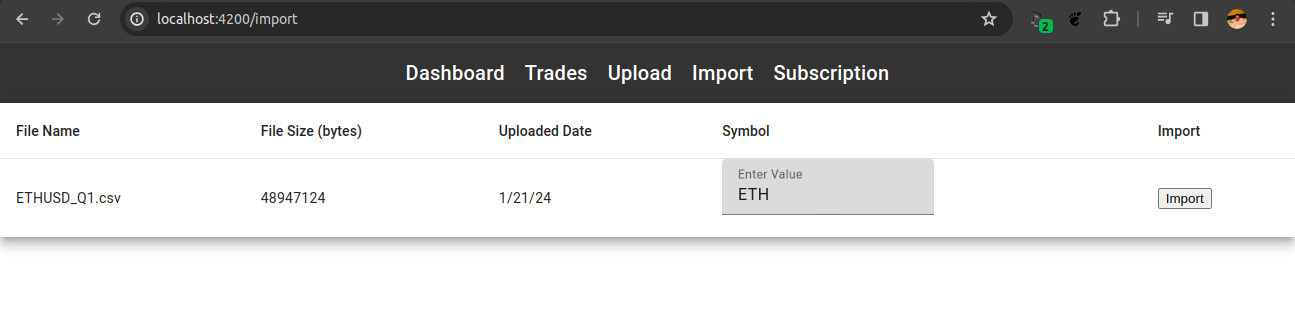
\includegraphics[width=\textwidth]{figures/frontend_import.png}
    \caption{Import}
    \label{fig:frontend_import}
\end{figure}

\subsubsection{Functionality}
The import section provides a streamlined process:
\begin{itemize}
    \item Displays a list of uploaded files, showing essential details like file name, size, and the date of upload.
    \item Allows users to associate each file with a specific symbol. This enables the user to add data from new symbols ensuring that the data is imported using the correct symbol.
    \item The \texttt{Import} button triggers the backend processes to parse the selected file, extract its contents, and import the data into the system's database.
\end{itemize}

\subsubsection{Workflow Integration}
The import functionality acts as a bridge between the initial file upload and the data's operational use within the system. It ensures that the data from the CSV files is properly validated, transformed, and stored, making it available for the system's analytical modules.

\subsubsection{User Empowerment}
This tab empowers users to manage the data lifecycle comprehensively, from uploading raw data files to initiating their integration into the system's core data structures. It is designed to handle large datasets, facilitating efficient data management and scalability.

In summary, the \texttt{Import} tab is a critical feature that encapsulates the system's capability to assimilate external data sources, providing users with control over when and how data is incorporated into the system.

\subsection{Subscription Management}

The \texttt{Subscription} tab (Figure \ref{fig:frontend_subscription}) is a dedicated interface within the frontend that allows users to add new currency pairs to the data collection service.

\begin{figure}[ht!]
    \centering
    
\includegraphics[width=\textwidth]{figures/frontend_subscription.png}
    \caption{Subscription}
    \label{fig:frontend_subscription}
\end{figure}

\subsubsection{Interface and Functionality}
This tab simplifies the process of adding new currency pairs for data collection:
\begin{itemize}
    \item Features a dropdown list that allows users to choose their preferred currency pair, such as \texttt{XRP}.
    \item The \texttt{Add} button is used to submit the request to the collector module, which then begins to monitor and collect data for the selected currency pair.
\end{itemize}

\subsubsection{User Empowerment}
This feature empowers users by giving them control over the scope of data collection, allowing for a personalized and relevant data set that aligns with their specific interests or trading strategies.

\subsubsection{System Scalability}
The ability to add new currency pairs on-the-fly demonstrates the system's scalability and adaptability to user needs and market changes. \\ \mbox{}
\\
In essence, the \texttt{Subscription} tab provides a vital function that ensures the system's data collection processes remain dynamic and user-driven, effectively expanding the system's analytical reach as new currency pairs are introduced into the marketplace. \\

    \chapter{User Guide}
Before deploying and running the system, certain prerequisites must be met to ensure a successful setup process. One of the primary requirements is the installation of Docker, which serves as the foundation for creating and managing the application's containers.
\newline
\\
For reference and reproducibility, the complete implementation described in this thesis is available in the accompanying source code repository: 
\url{https://github.com/rileydavid/kraken-lstm-prediction-engine}

\section{Prerequisites}

\subsection{Docker Installation}
To run this application, Docker must be installed and properly configured. The following steps have to be successfully completed:

\begin{enumerate}
    \item \textbf{Download Docker}: Visit the official Docker website at \url{https://www.docker.com/get-started} and download the appropriate Docker Desktop application for your operating system.
    \item \textbf{Install Docker}: Execute the installer and follow the on-screen instructions to install Docker on your machine. Ensure that the neeeded administrative privileges are available to complete the installation.
    \item \textbf{Verify Installation}: Open a terminal or command prompt and run the command \texttt{docker ---version} to verify that Docker has been installed correctly. The Docker version number should show up in the output.
    \item \textbf{Post-Installation Steps}: Depending on the host operating system, there may be additional post-installation steps required. These are detailed in the Docker documentation and ensure that Docker runs smoothly.
\end{enumerate}

\subsection{Historical Dataset}
\label{section:historical_dataset}
To make sure the frontend is fully functional and to enable predictions the historical data for the currency pair \texttt{ETH/USD} is needed, which can be downloaded from \url{https://support.kraken.com/hc/en-us/articles/360047543791-Downloadable-historical-market-data-time-and-sales-}. Download the full dataset as well as the incremental update for 2023 Q3 and optionally Q4. 

\section{Starting the Application}

To start the application, follow the steps below. Ensure you are in the root directory of the project, where the \texttt{docker-compose.yaml} file is located.

\begin{enumerate}
\item \textbf{Start Docker:} Run the following command in a terminal or command prompt:
\begin{verbatim}
docker-compose --env-file config.env up --build
\end{verbatim}
This will build all necessary container images and start them afterwards. This process might take a while as it is pulling in dependencies and compiling the source code. 

\item \textbf{Access MinIO Dashboard:} Navigate to the MinIO dashboard at \url{http://172.1.0.12:2001/}. Log in using the credentials from the \texttt{config.env} file. The default credentials are:
\begin{verbatim}
MINIO_ROOT_USER=minio_root_user
MINIO_ROOT_PASSWORD=minio_password
\end{verbatim}

\item \textbf{Create a Bucket:} Create a bucket named \texttt{prod-model} (Figure \ref{fig:minio_create_bucket}).

\begin{figure}[ht!]
    \centering
    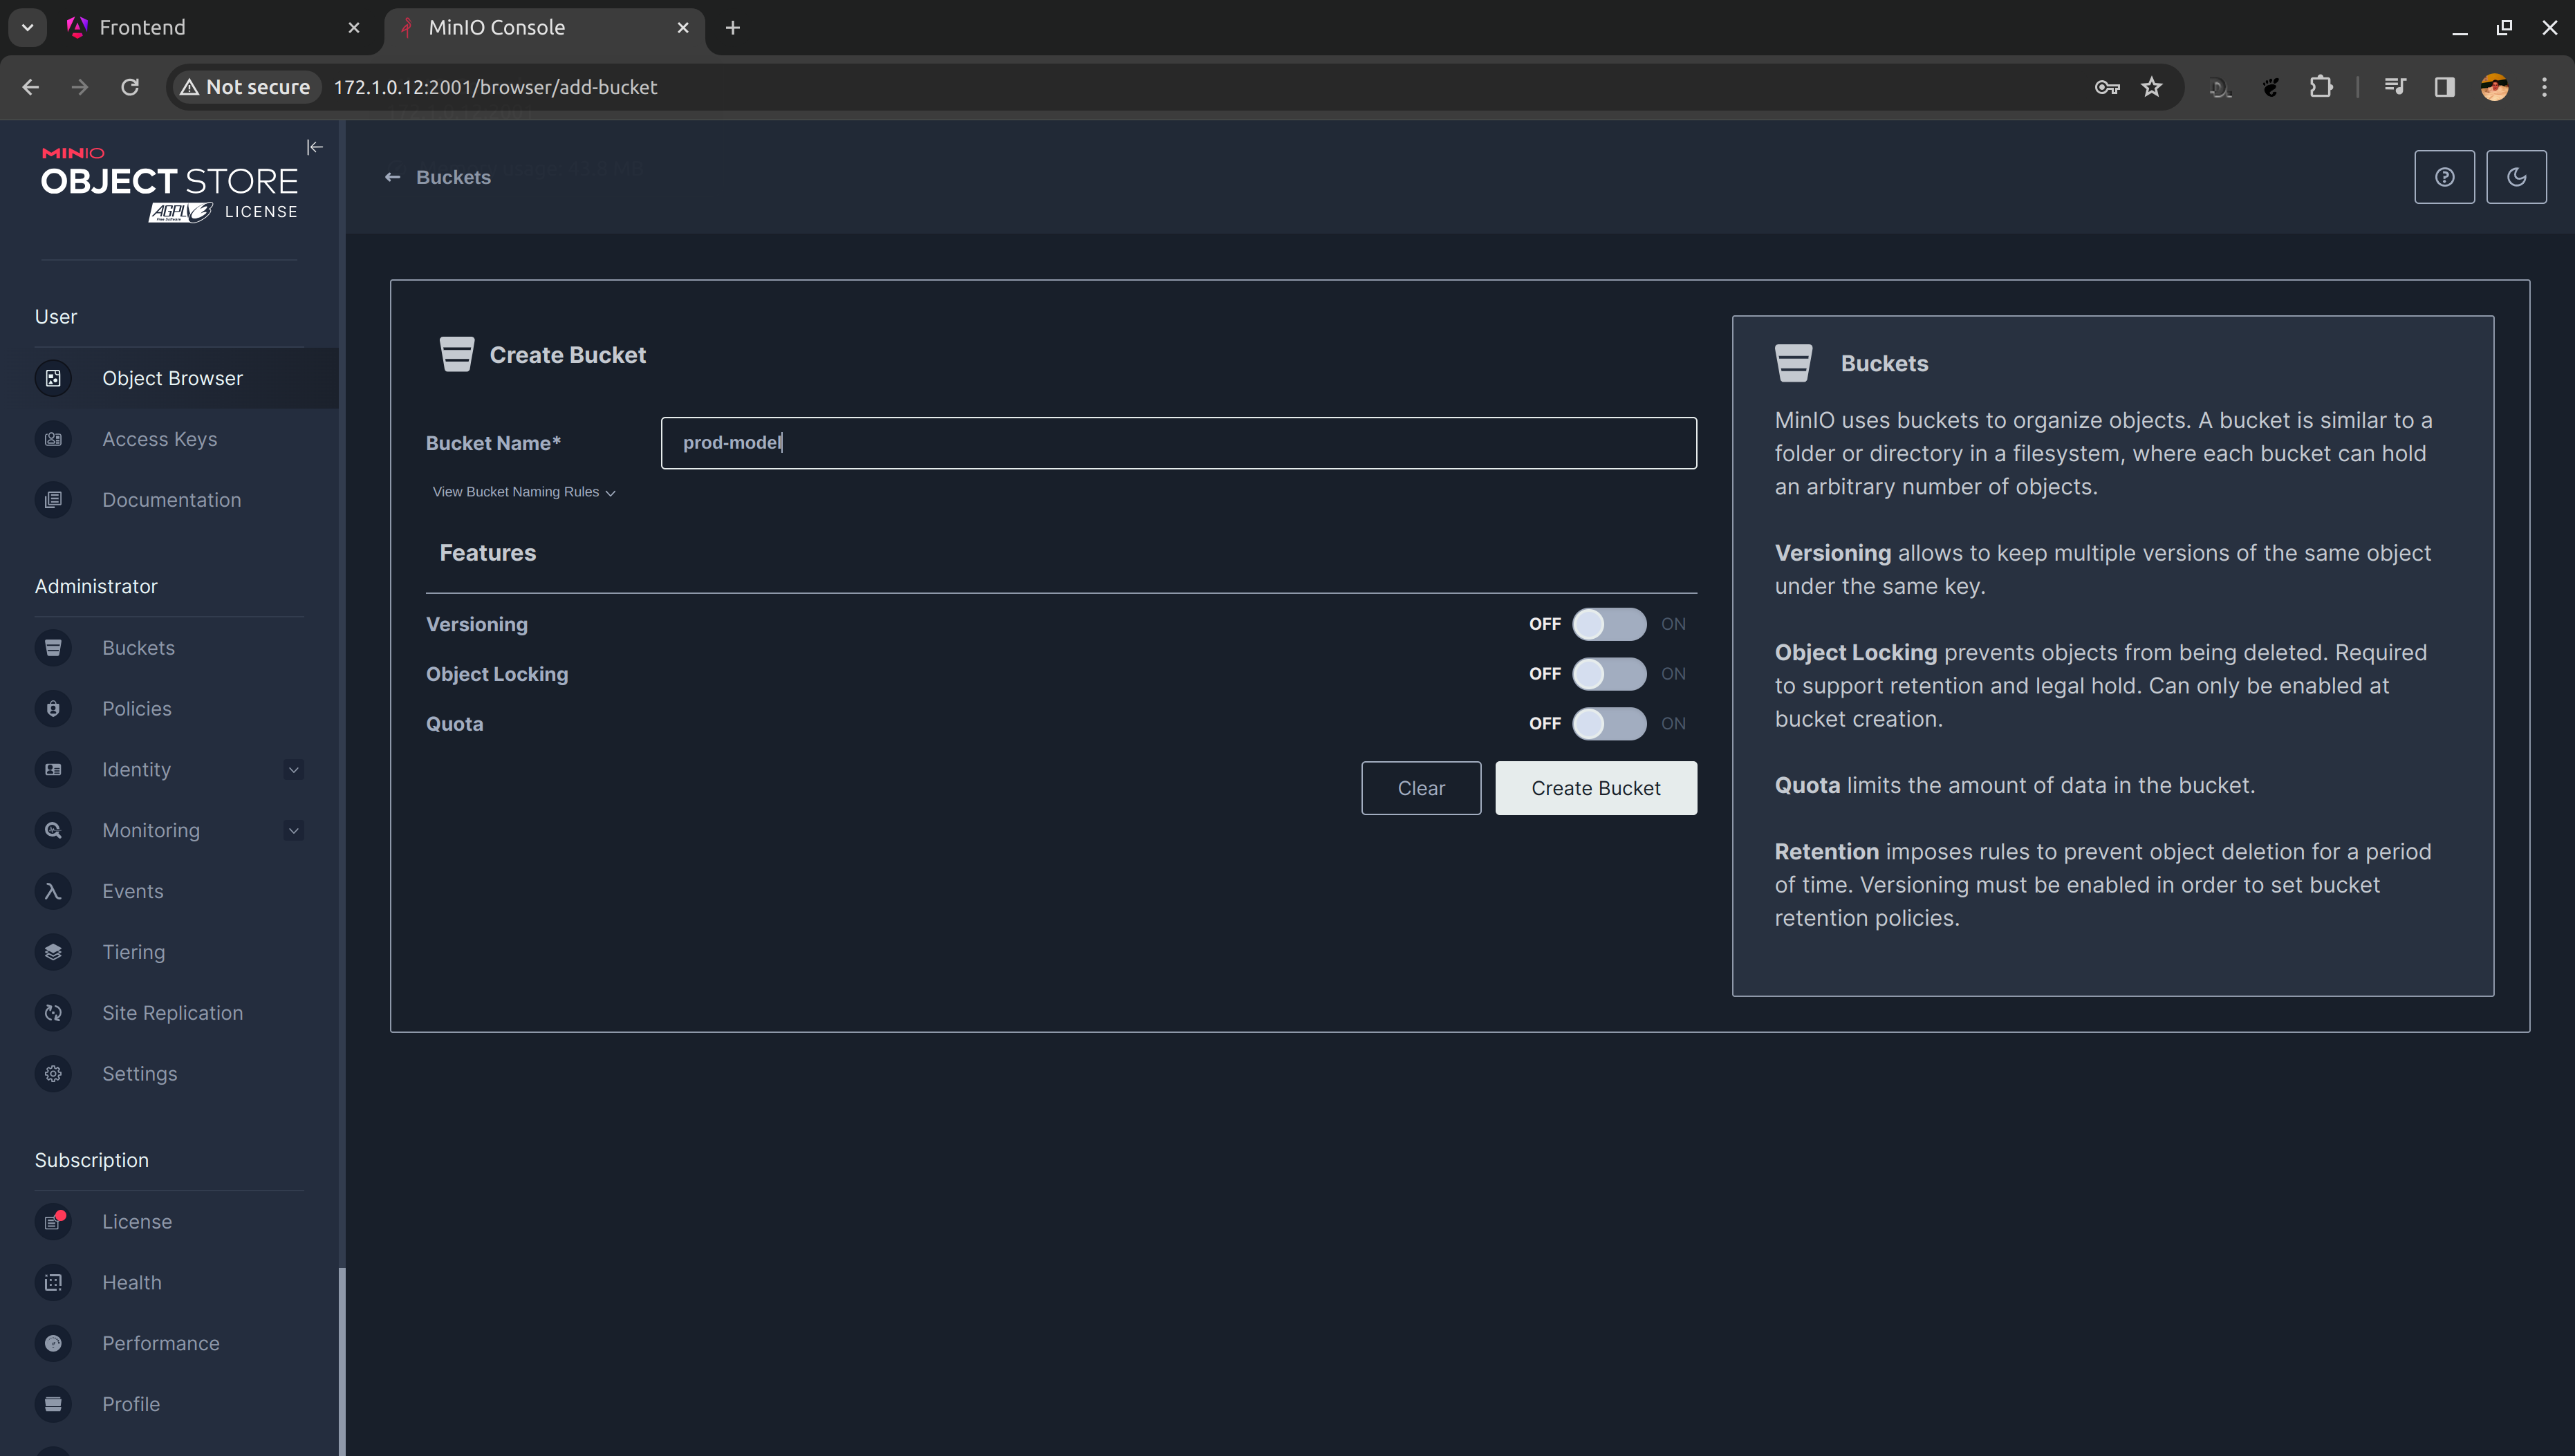
\includegraphics[width=\textwidth]{figures/create_bucket.png}
    \caption{Create Bucket in Minio}
    \label{fig:minio_create_bucket}
\end{figure}

\item \textbf{Upload Model File:} Upload the \texttt{clean-mare-368.pkl} file from the \texttt{data/model} folder to the \texttt{prod-model} bucket.

\item \textbf{Update Access Keys:} Create new access keys (Figure \ref{fig:minio_create_accesskeys}) and update them in the \texttt{config.env} file:
\begin{verbatim}
MINIO_ACCESS_KEY=eITEO5kyE7hccuy7UTHv
MINIO_SECRET_ACCESS_KEY=5KBCscit30Z70bSVGIMvMBBoqV8ydn232o2MW9RA
\end{verbatim}

    \begin{figure}[H]
    \centering
    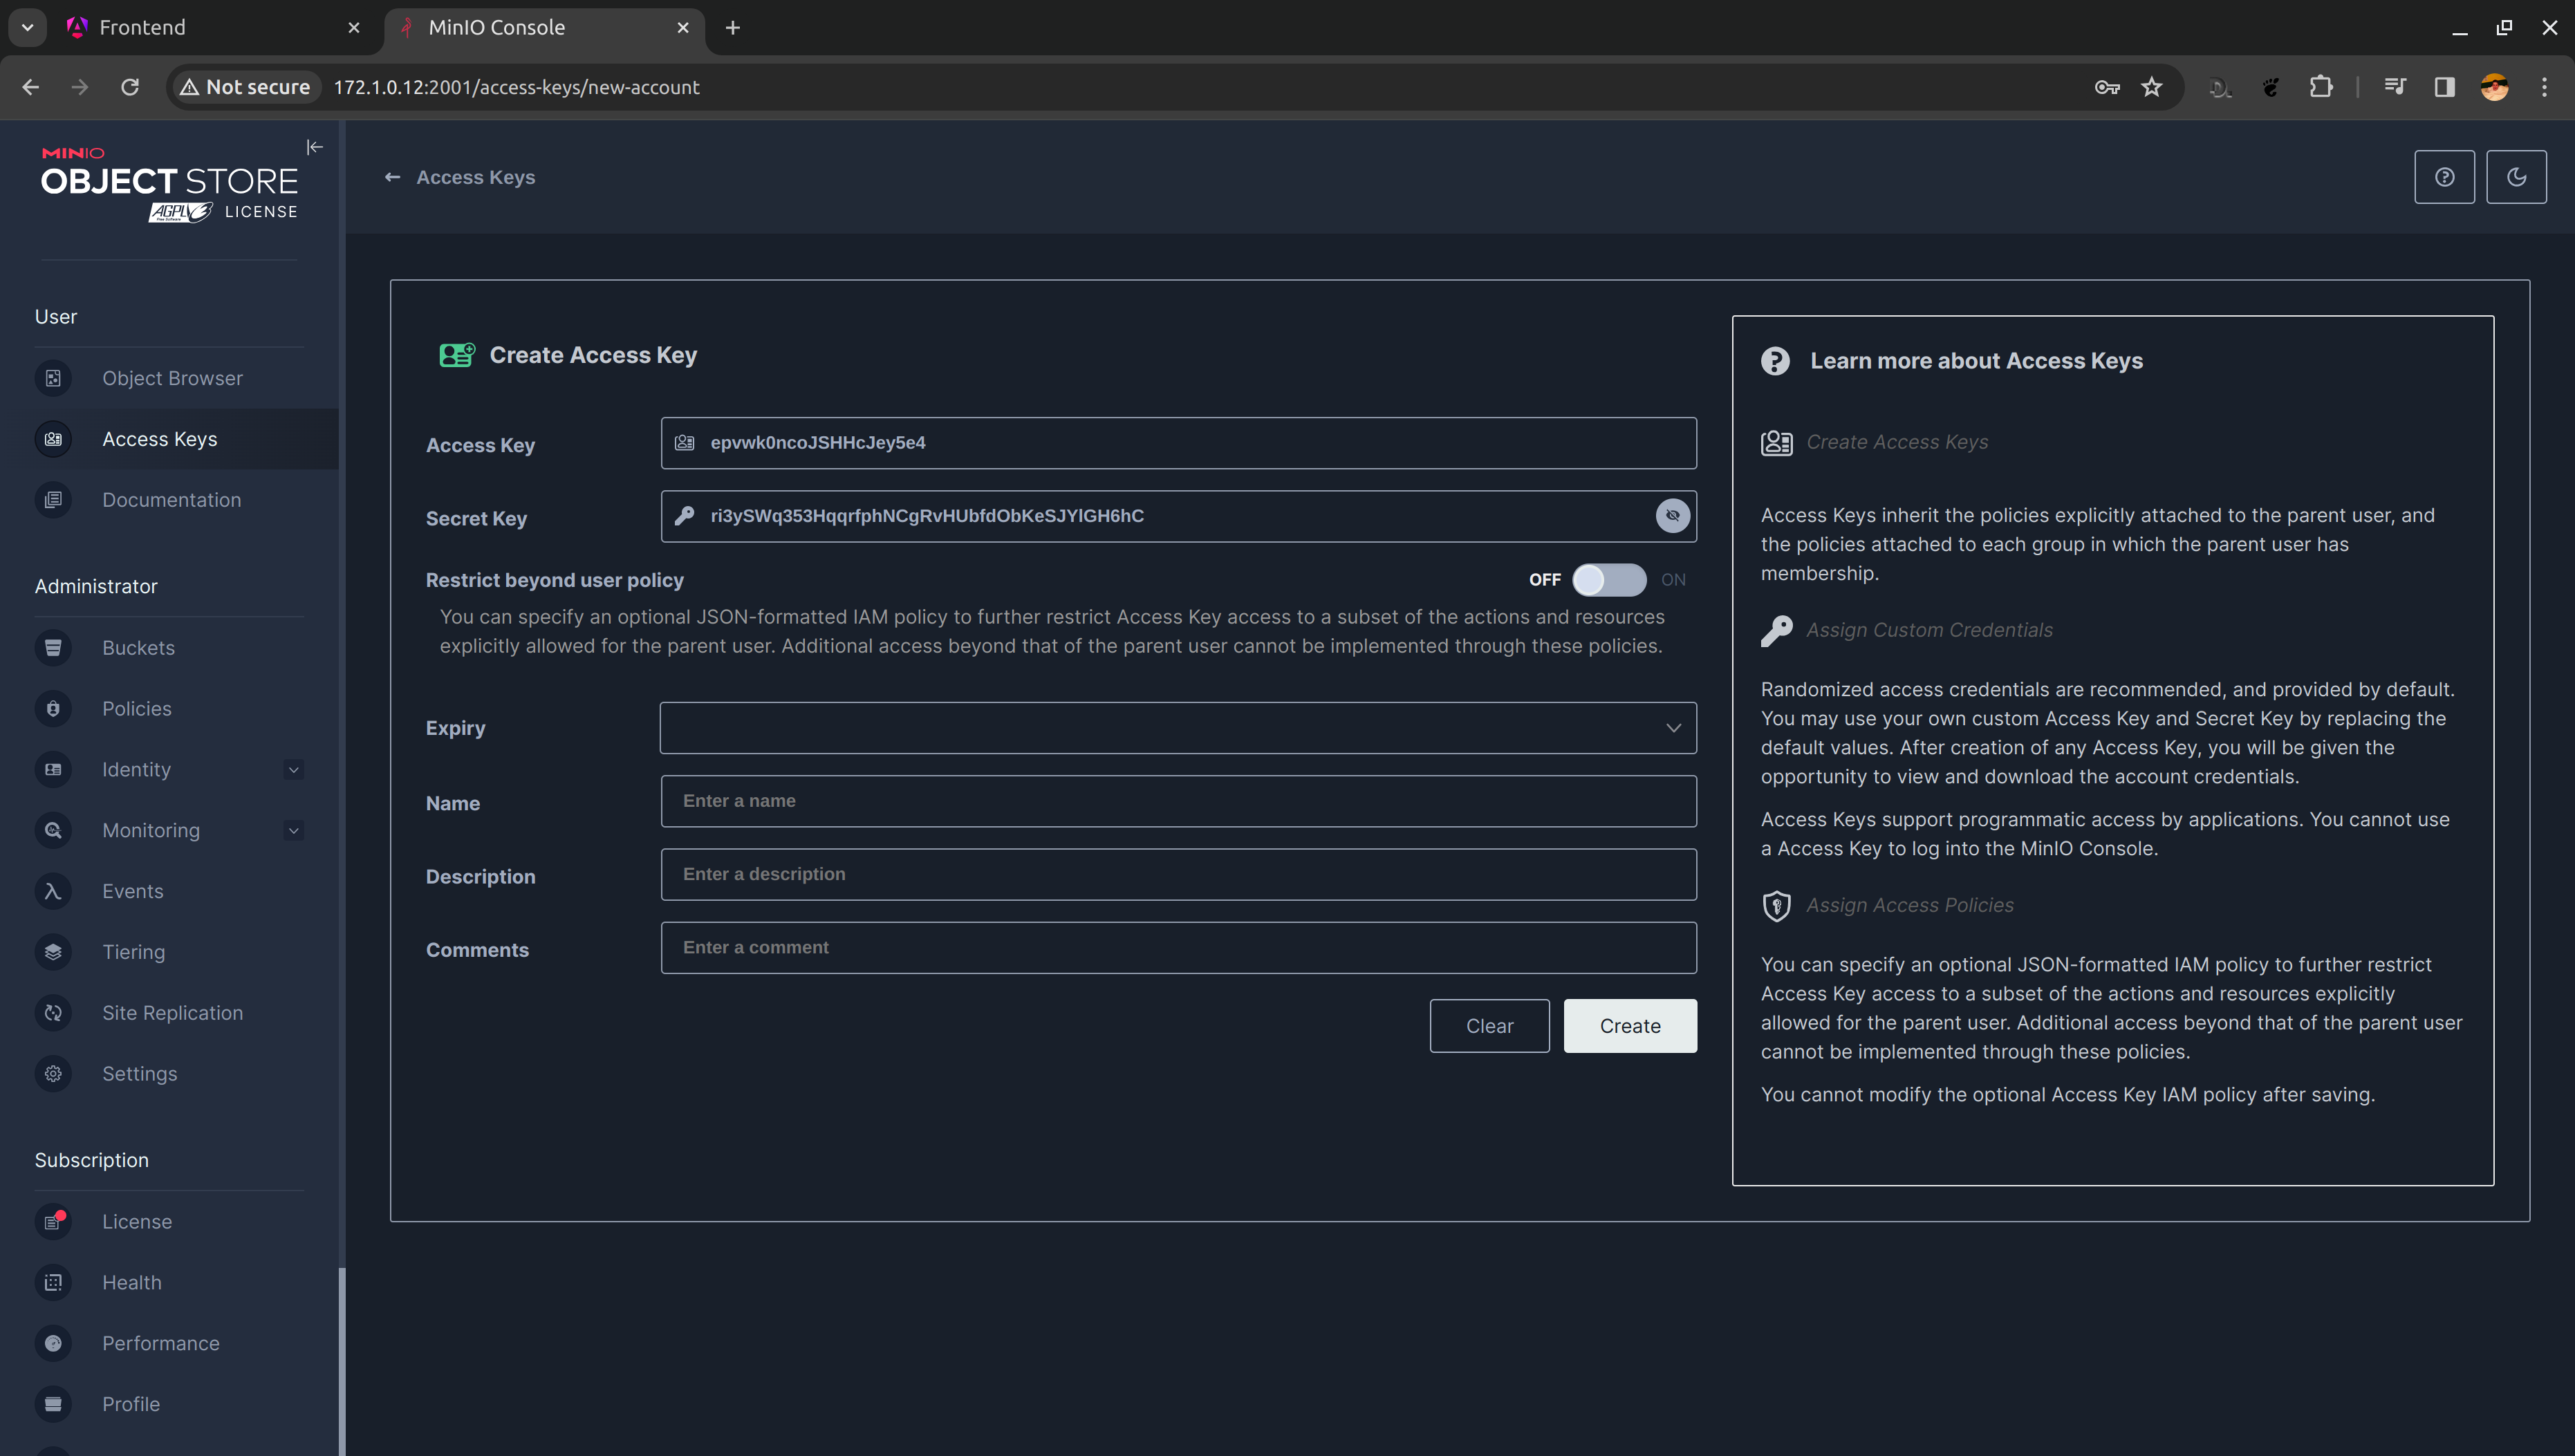
\includegraphics[width=\textwidth]{figures/accesskey_generate.png}
    \caption{Create Access Keys in Minio}
    \label{fig:minio_create_accesskeys}
\end{figure}

\item \textbf{Restart Docker:} Execute the following commands to restart the services:
\begin{verbatim}
docker-compose --env-file config.env down
docker-compose --env-file config.env up --build
\end{verbatim}

\item \textbf{Open Frontend:} After the docker containers have started, open the frontend in a browser: \url{http://localhost:4200}.

\item \textbf{Upload:} Navigate to the \texttt{Upload} tab on the Frontend and upload the historical data for \text{ETH/USD} (Section \ref{section:historical_dataset})

\item \textbf{Import:} To import the just uploaded .csv files navigate to the \texttt{Import} tab and import the necessary files by entering the sybmol \texttt{ETH} and start the import using the import button. Currently it is only possible to add USD currency pairs as the backend automatically fills in the USD part.  

\item \textbf{Dashboard: } Now the main functionality of the system is ready. Try it out by navigating to the Dashboard and selecting the \texttt{ETH/USD} symbol and press fetch.
\end{enumerate}

\section{Model Tuning (Optional)}
To run the Model-tuning Script all libraries used have to be installed locally. \\

\begin{table}[H]
\centering
\begin{tabular}{ll}
\hline
\textbf{Name}         & \textbf{Version} \\ \hline
Python Kernel & 3.10.12      \\
numpy         & 1.23.5       \\
pandas        & 1.5.2        \\
more-itertools & 9.0.0       \\
mlflow        & 2.8.0        \\
keras         & 2.14.0       \\
ipython       & 8.7.0        \\
matplotlib    & 3.6.2        \\
scikit-learn  & 1.1.3        \\
holidays      & 0.32         \\ \hline
\end{tabular}
\caption{Software and Libraries Version List}
\label{tab:software_version}
\end{table}

Additionally it can be beneficial to install Nvidia CUDA \cite{NVIDIACUDAToolkit} to improve training performance, keep in mind that this is only a viable option if a Nvidia GPU is installed in the system. To run the model-tuning script (located in the \texttt{prediction-model-development} folder), replace the \texttt{AWS\_ACCESS\_KEY\_ID} and the \texttt{AWS\_SECRET\_ACCESS\_KEY} with the generated MinIO keys from earlier. The dataset required is available in the folder and therefore does not have to be exported using PgAdmin. \\
\begin{verbatim}
os.environ["AWS_ACCESS_KEY_ID"] = "eITEO5kyE7hccuy7UTHv"
os.environ["AWS_SECRET_ACCESS_KEY"] = "5KBCscit30Z70bSVGIMvMBBoqV8ydn232o2MW9RA"
\end{verbatim}

\section{PgAdmin}
\label{section:pgadmin_user_guide}
\subsection{Login and Configuration}
To make use of the export feature of \texttt{PgAdmin} navigate to \url{http://localhost:5050/} and login using the credentials configured in the \texttt{config.env} file (Section \ref{docker_config_env}). The landing page of \texttt{PgAdmin} (Figure \ref{fig:pgadmin_landing_page}) should open. 

\begin{figure}[H]
    \centering
    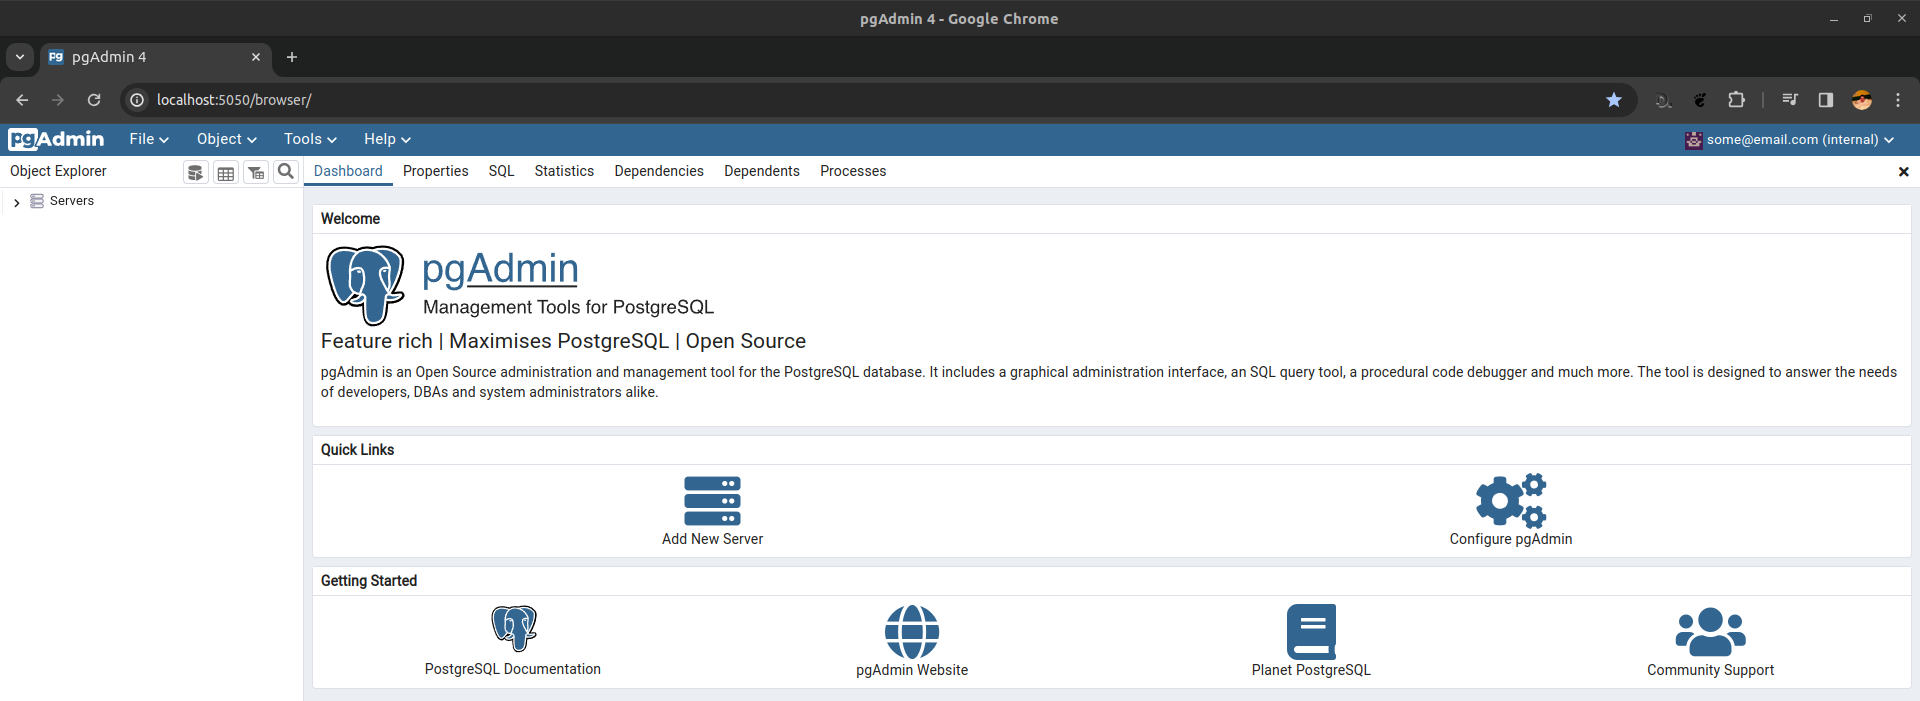
\includegraphics[width=\textwidth]{figures/pgadmin_landing_page.png}
    \caption{PgAdmin Dashboard}
    \label{fig:pgadmin_landing_page}
\end{figure}

On the landing page (Figure \ref{fig:pgadmin_landing_page}) press the add new server button. A dialog (Figure \ref{fig:pgadmin_add_server_page}) should open up. Enter a fitting name (e.g. \texttt{timescale}) and navigate to the \texttt{Connection} tab. 

\begin{figure}[H]
    \centering
    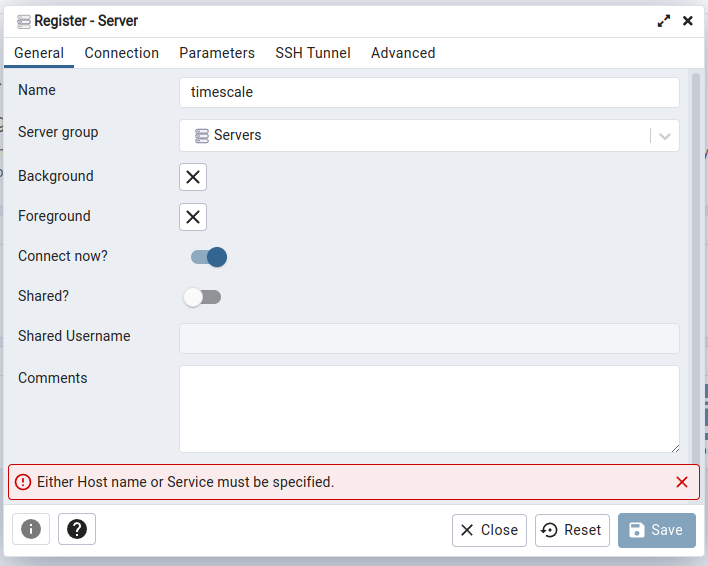
\includegraphics[width=0.75\textwidth]{figures/pgadmin_add_server_page.png}
    \caption{PgAdmin Add Server Dialog}
    \label{fig:pgadmin_add_server_page}
\end{figure}

After navigating to the \texttt{Connection} tab (Figure \ref{fig:pgadmin_server_ip_setup}) enter the IP-Address of timescale, \texttt{172.1.0.10}, if the default configuration has not been adapted. Enter the user and password for timescale, the default values are \texttt{admin} and \texttt{password} (Section \ref{docker_config_env}), and press save.  
\begin{figure}[H]
    \centering
    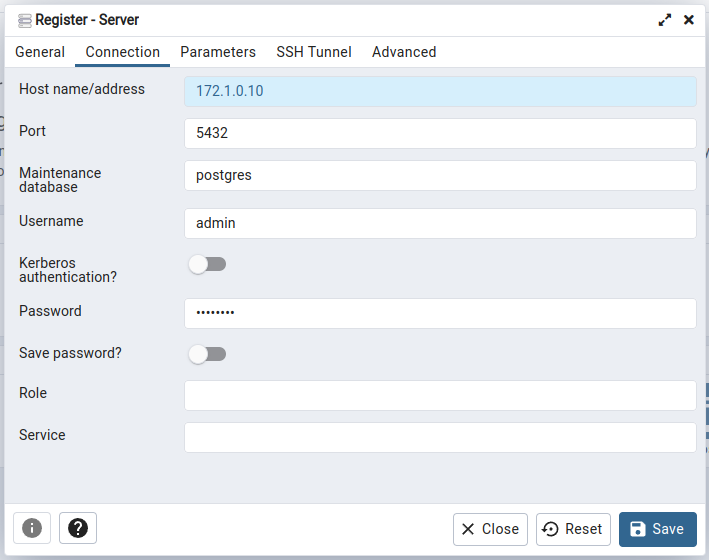
\includegraphics[width=\textwidth]{figures/pgadmin_server_ip_setup.png}
    \caption{PgAdmin Connection Tab}
    \label{fig:pgadmin_server_ip_setup}
\end{figure}

\subsection{Exporting Data}
To export data for training purposes press the \texttt{Tools} option in the menu bar and select the query tool (Figure \ref{fig:pgadmin_export}). Use the query text-field to run the following query (Listing \ref{lst:pg_query}): 

\begin{lstlisting}[language=sql, caption={ETH/USD Training Dataset Query}, label={lst:pg_query}]
SELECT * FROM ohlc_hour 
    WHERE symbol_id = 1 
    AND bucket >= '2020-01-01 00:00:00+00' 
    AND '2023-09-30 23:00:00+00' >= bucket 
    ORDER BY bucket ASC;
\end{lstlisting}

In the data output section use the download button to download this dataset as a .csv. 
\newpage
\begin{figure}[H]
    \centering
    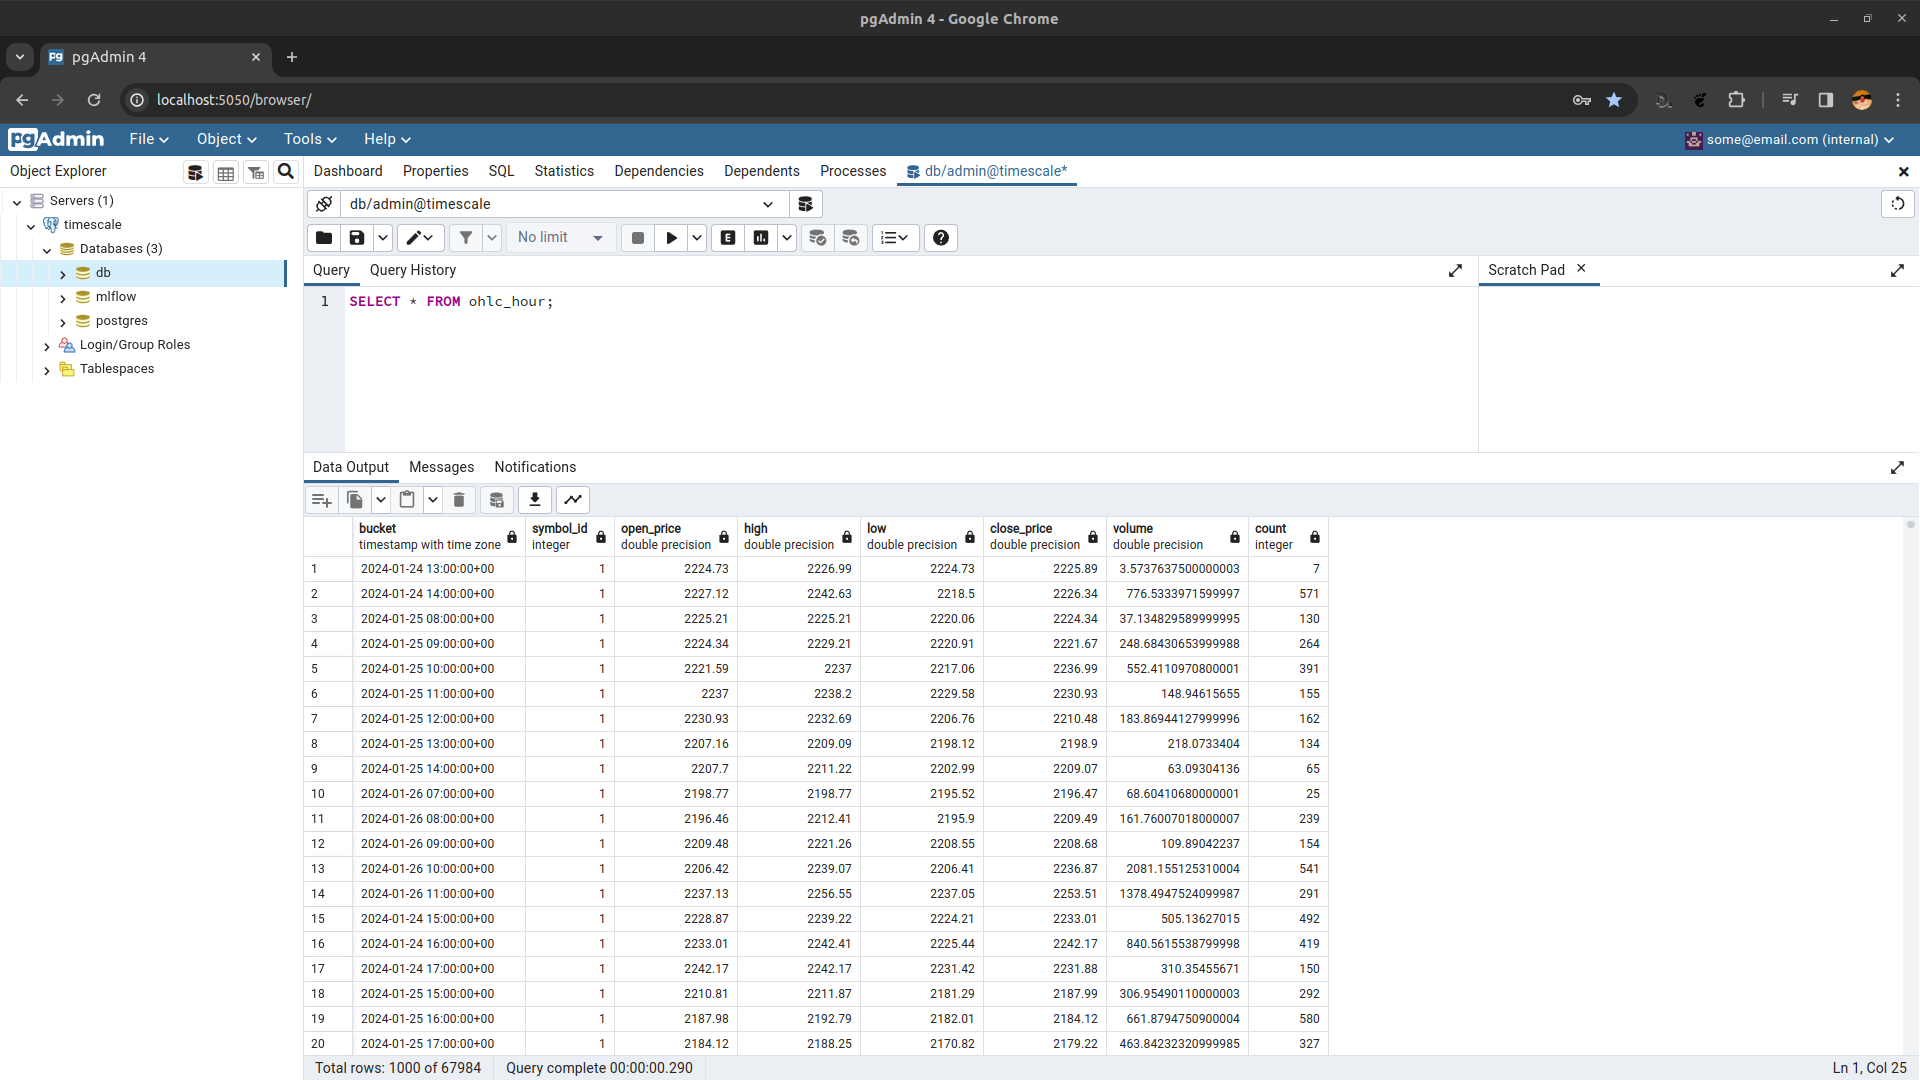
\includegraphics[width=\textwidth]{figures/pgadmin_export.png}
    \caption{PgAdmin Export}
    \label{fig:pgadmin_export}
\end{figure}


    \chapter{Justification and Evaluation}


\section{Justification}

The relevance of deploying advanced machine learning models for financial markets cannot be overstated, especially in the context of cryptocurrency markets with their inherent volatility, unpredictability, and the significant financial opportunities it presents. Cryptocurrencies, unlike traditional financial assets, exhibit swift price fluctuations and unique market dynamics, driven by a myriad of factors ranging from technological advancements to regulatory changes and investor sentiment. This unpredictability, while posing considerable risks, also opens up substantial opportunities for market participants equipped with the right tools to interpret and anticipate market movements.\\

In this high-stakes environment, a well-crafted predictive model can serve as a powerful tool, offering users a significant edge. By harnessing advanced machine learning techniques to analyze and interpret market data, such models can uncover hidden patterns and trends that may elude traditional analysis, enabling users to make more informed, data-driven decisions.\\

Furthermore, the successful implementation of this framework in the cryptocurrency domain lays a robust foundation for its application in other financial markets. The model's adaptability and learning capabilities could potentially be extended to traditional fiat currencies, such as the US Dollar or Euro, and even equities, thereby broadening the scope of its applicability and impact. In essence, this research not only addresses the immediate challenges posed by the cryptocurrency market but also paves the way for additional financial modeling and analysis techniques that could provide significant insights in market operations. \\

In a domain where timely and accurate information is paramount, the development of such predictive models is not merely an academic exercise but a necessary evolution to meet the complex demands of modern financial markets. This research is a step towards realizing that goal, offering promising avenues for both immediate application in the cryptocurrency market as well as potential future expansions. \\

Central to the designed framework is the comprehensive data collection system, which serves as the lifeblood for any machine learning application. By ensuring the availability of high-quality, real-time market data, the framework sets the stage for precise and insightful market predictions. \\

Key to the framework's utility is its focus on continuous improvement. The systematic training and fine-tuning of the model's hyperparameters are instrumental in adapting to the market's evolving dynamics. This iterative approach not only refines the models accuracy over time but also embeds a culture of perpetual enhancement within the framework's architecture. The incorporation of robust experiment tracking mechanisms ensures that each iteration is documented, paving the way for transparent and informed advancements in the model's development. \\

The practical implications of this framework extend far beyond its technical footprint. For traders and investors, the framework promises a new platform for data-driven insights. This is achieved by harnessing the predictive power of advanced machine learning techniques. The framework offers a tool that can potentially uncover market trends and investment opportunities that might be obscure or latent in raw market data. This level of analysis can empower traders and investors with a more nuanced understanding of market movements, enabling them to make more informed and strategic decisions. \\

Moreover, the framework's modular and adaptable architecture ensures that it can remain at the forefront of technological advancements. As new machine learning techniques and analytical tools emerge, the framework is well-positioned to integrate these innovations, continually enhancing its predictive capabilities. \\

In essence, this research is not just about building a sophisticated predictive model, it is about crafting a dynamic, evolving tool that grows in intelligence and insight. It is about offering traders and investors a lens through which the complexities of the cryptocurrency market are not just seen, but also understood and anticipated. The real-world benefits, therefore, are not only imminent but also potentially transformative, redefining the landscape of financial decision-making in the digital age. \\

\subsection{Future Scope}

As the framework continues to evolve, the integration and enhancement of its core components present promising avenues for advancement. A significant leap forward would involve the consolidation of the Rust backend and the model service, morphing them into a singular, powerful entity within the system. This transformation is not merely about streamlining the architecture but also about harnessing the full potential of Rust's performance, stability, and memory safety features. \\

The Rust ecosystem is rapidly gaining momentum in the domain of machine learning. Libraries such as Burn \cite{burnDev}, PyO3 \cite{PyO3PythonFromRust}, and TensorFlow bindings \cite{tensorflowRust} for Rust are laying the groundwork for a new paradigm in machine learning infrastructure, one where Rust's efficiency and robustness can be leveraged to its full extend. The strategic integration of these libraries and technologies could redefine the framework's operational efficiency, making it a formidable tool in processing and analyzing large volumes of financial data. \\

The envisioned future of this framework is one where Python's versatility in machine learning is combined with Rust's performance-oriented nature. This synergy aims to reduce the framework's dependency on Python, not by displacing it, but by optimizing the computational-intensive aspects of the system with Rust's capabilities. Such an approach promises not only a boost in performance but also an enhancement in the system's reliability and resource efficiency.

Furthermore, this evolution is not just about technological transformation but also about positioning the framework at the forefront of innovation in financial analytics. As machine learning continues to advance, the framework's adaptable and forward-looking architecture ensures it remains relevant and capable of incorporating cutting-edge methodologies and tools. 
\\
In conclusion, the road map for the framework's development is clear and ambitious. It involves not just incremental improvements but a strategic reorientation towards a more integrated, efficient, and cutting-edge system. This vision, when realized, will not only enhance the framework's capabilities but also redefine its role and impact in the domain of financial market analytics.
 
\section{Evaluation}

\subsection{Methodology Assessment}
Detailed in Section \ref{section:model_evaluation} it becomes evident that the current models, despite their sophisticated architecture, fall short of the accuracy and reliability required to guide users in making sound financial decisions. The performance limitations are underscored by the metrics used: Mean Absolute Error (MAE), Mean Squared Error (MSE), Explained Variance Score, R-squared Score, Root Mean Squared Error (RMSE), and Mean Absolute Percentage Error (MAPE). While these metrics provide a quantitative measure of the model's predictive capabilities, their collective insights suggest that the models may not fully capture the complexities of the cryptocurrency market dynamics. \\ 

The reliance on these metrics, primarily centered around error minimization and variance explanation, might be insufficient to holistically evaluate the model's predictive performance. In the context of financial decision-making, where the cost of false positives and false negatives can be high, it is crucial to consider metrics that reflect the model's ability to balance precision and recall. Incorporating Precision, Recall, and the F1-score into the evaluation framework could provide a more nuanced understanding of the model's performance, particularly in terms of their ability to accurately predict significant market movements. \\

Precision would offer insight into the model's ability to minimize false positives, a critical factor when predicting price movements in volatile markets. Recall would shed light on the model's ability to accurately identify actual positive occurrences, which is essential to ensure no significant investment opportunities are missed. Lastly, the F1-score, as a harmonic mean of precision and recall, would provide a single metric to assess the balance between precision and recall, offering a more balanced view of the model's predictive accuracy. \\

In addition to the conventional evaluation metrics utilized, it is crucial to consider the dynamic nature of model performance during training. Monitoring the evolution of model loss throughout the training process, alongside visualizing the performance on the validation set, can provide valuable insights into the model's learning trajectory.  \\
The absence of a specified seed for \texttt{TensorFlow} and \texttt{numpy} during the model tuning process introduces an element of unpredictability, hindering the re-producibility of model training. To enhance the robustness of model tuning the establishment of a seed would ensure consistency across different runs. By incorporating these practices, the evaluation framework would gain significant depth, offering a more comprehensive understanding of the model's predictive capabilities, and aiding in the refinement of future model iterations.

\subsection{Data Quality and Reliability}
The data collection mechanism, established through the Kraken Websocket API, has demonstrated reliability and consistency during the testing phase, underscoring the robustness of the underlying infrastructure. However, there are opportunities to fortify the system further and enhance the data's integrity and utility. \\

One notable limitation is the system's current inability to manage unexpected interruptions such as connection timeouts or errors. The absence of an automated re-connection protocol could lead to gaps in the data, potentially undermining the model's training and predictive accuracy. Implementing a monitoring mechanism for heartbeat signals from the API and logging any anomalies could significantly mitigate this risk. By documenting instances of potential data loss and promptly re-establishing connections, the system would be able to ensure a more continuous and reliable data stream. \\

Additionally, the data aggregation strategy should be refined to maximize flexibility and granularity. While the current framework aggregates data on an hourly basis, providing the capability to create Open, High, Low, Close (OHLC) aggregates on a 1-minute basis and subsequently aggregating these into larger time frames (e.g., 5 minutes, 15 minutes, 1 hour, etc.) on demand would offer enhanced granularity. This flexibility would not only cater to diverse analytical needs but also enable more nuanced model training. \\

Moreover, integrating core metrics such as moving averages directly into the database aggregation process, rather than computing them in the model service, could streamline operations and provide direct access to these key indicators. This integration would not only reduce computational overhead in the model service, but also offer potential for real-time analytical insights, enhancing the user experience by providing immediate access to these critical metrics. \\

In conclusion, while the data collection and processing mechanisms exhibit a strong foundation, the proposed enhancements in error handling, data aggregation flexibility, and integration of core metrics into the database would elevate the system's robustness and precision. These improvements are pivotal in ensuring that the data infrastructure can support more advanced predictive models and ultimately lead to a more informed and effective decision-making processes. \\

\subsection{Infrastructure}
The technology stack, despite its robust architecture and comprehensive suite of services, encounters a notable bottleneck with Timescale's performance. This issue persists despite the implementation of indexes aimed at optimizing query efficiency, indicating a more complex challenge. \\

The system's infrastructure is extensive: a Node.js/Angular frontend hosted in a Docker container with Nginx using multiple workers, an MLflow webserver and model service both operating with multiple workers, a multi-threaded Rust backend with one thread dedicated to continuous data collection, and MinIO providing S3 storage services. This multifaceted setup places considerable demand on the CPU, particularly in the context of a development environment concurrently running applications like VS Code and Chrome. \\

In light of these insights, the observed latency in Timescale might be attributed to the cumulative load from the various services and the development environment itself, rather than the database's intrinsic limitations. Transitioning to a dedicated server for Timescale, equipped with robust hardware specifications, is anticipated to alleviate this bottleneck significantly. This would ensure that the database's performance is optimized, without being hindered by the extensive computational demands of the diverse services and development tools. \\

Moreover, the model tuning script, crucial for refining the predictive models, currently operates locally due to complexities in integrating a Jupyter notebook server with CUDA in a docker container. This setup, while necessary for harnessing GPU acceleration, does not align with the mentality of this research to utilize Docker for enabling the framework to run anywhere.\\

By addressing these infrastructure challenges and optimizing the computational allocation, the system could achieve a harmonious balance between its extensive components, ensuring seamless performance and robust support for cryptocurrency market analysis and predictions. \\

\subsection{Model}

To evaluate the LSTM models performance properly, two baseline models, Moving Average (MA) and Last Value, were established. This comparative analysis was aimed at providing a comprehensive understanding of the LSTM's capabilities in the context of predictive analytics. The Last Value model (Figure \ref{fig:last_value_forecast}), serving as a rudimentary baseline, operates under a simple premise predicting future values based solely on the most recent observation. Surprisingly, this approach demonstrated significant efficacy, reflected in its superior performance metrics: it achieved the lowest Mean Squared Error (MSE) at 23.52, the lowest Mean Absolute Error (MAE) at 3.24, and the highest R\(^2\) Score and Explained Variance Score, both at 0.975 (Table \ref{tab:metrics_comparison}). Such outcomes not only highlight the Last Value models effectiveness but also challenge the conventional wisdom that more complex models inherently offer better forecasting accuracy. This is particularly noteworthy in scenarios where the latest data point is a strong predictor of future trends. \\

\begin{figure}[H]
    \centering
    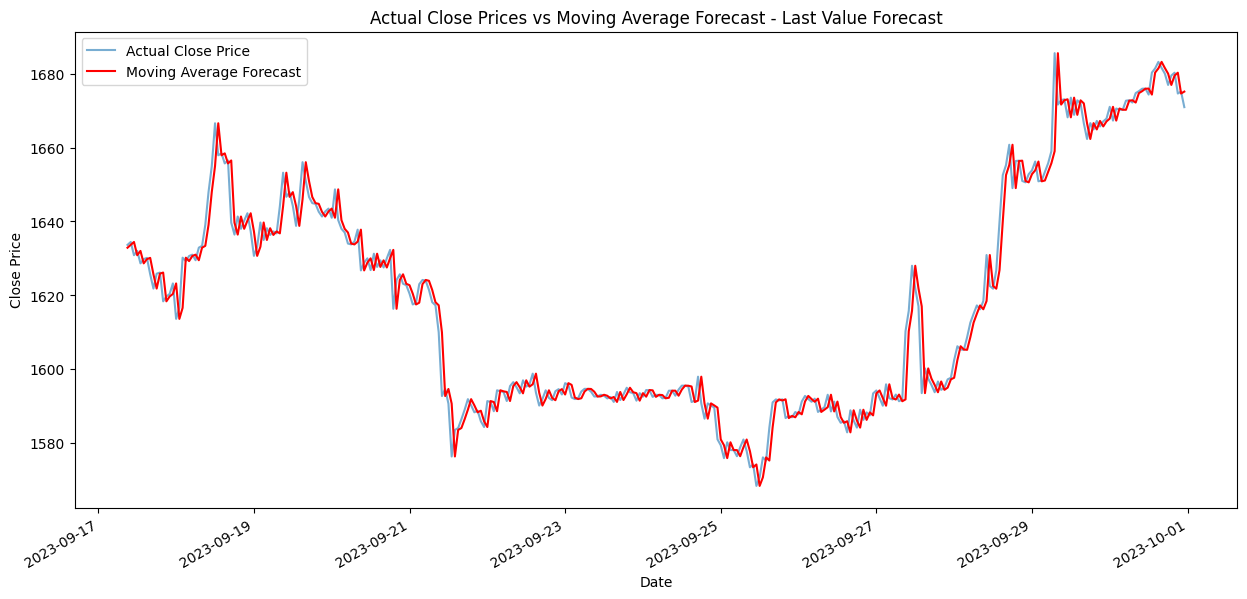
\includegraphics[width=\textwidth]{figures/last_value_model_forecast.png}
    \caption{Last Value Forecast Performance}
    \label{fig:last_value_forecast}
\end{figure}


The Moving Average model (Figure \ref{fig:ma_model_forecast}), which calculates predictions based on the average of the last five data points, was selected as a slightly more sophisticated baseline. Despite its simplicity, it too yielded impressive results (Table \ref{tab:metrics_comparison}), with an MSE of 46.54 and an MAE of 4.41. Its R\(^2\) Score and Explained Variance Score, both at 0.951, further attest to its capability to adequately capture the underlying trends in the data. These findings underscore the potential of simple statistical methods to provide reliable forecasts, challenging the premise that advanced models are always necessary for accurate predictions. \\

\begin{figure}[H]
    \centering
    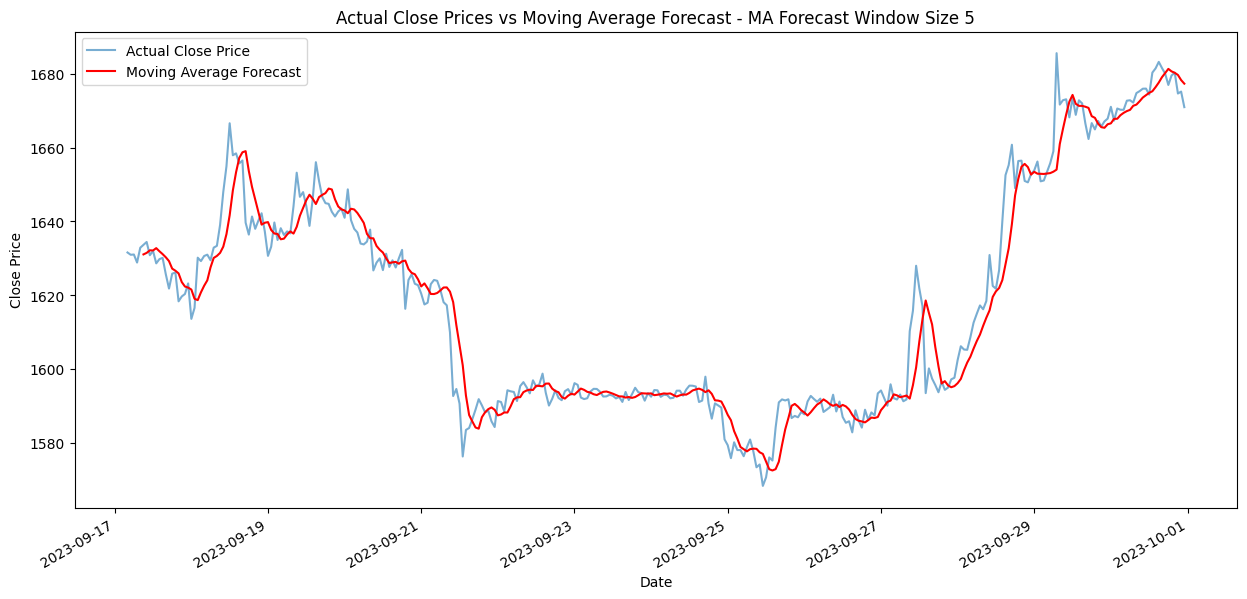
\includegraphics[width=\textwidth]{figures/ma_model_forecast.png}
    \caption{Moving Average Model Forecast Performance}
    \label{fig:ma_model_forecast}
\end{figure}

In contrast, the LSTM model, designed to leverage long-term dependencies in data, exhibited lower performance relative to the baseline models (Table \ref{tab:metrics_comparison}). With the highest MSE of 121.07, an MAE of 8.74, and the lowest R\(^2\) Score of 0.88, the LSTM's results were somewhat disappointing. This underperformance raises important considerations regarding the application of complex neural networks like LSTMs in forecasting tasks, especially when simpler models can achieve comparable or superior results under certain conditions. \\ 


\begin{table}[H]
\centering
\begin{tabular}{|l|c|c|c|}
\hline
Metric & Moving Average & Last Value & LSTM (clean-mare-368) \\ 
\hline
Mean Squared Error & 46.54 & 23.52 & 121.07 \\
Mean Absolute Error & 4.41 & 3.24 & 8.74 \\
Root Mean Squared Error & 6.82 & 4.85 & 11 \\
Mean Absolute Percentage Error& 27.18\% & 19.94\% & 54.04\% \\
R\(^2\) Score & 0.951 & 0.975 & 0.88 \\
Explained Variance Score & 0.951 & 0.975 & 0.897 \\
Timesteps & 327 & 327 & 327 \\
\hline
\end{tabular}
\caption{Comparison of Metrics Across Three Models}
\label{tab:metrics_comparison}
\end{table}

The consistent timesteps across all models ensure a level playing field for comparison, further validating the conclusions drawn from the data. This research illustrates the vital lesson that in forecasting, simpler models can not only serve as valuable benchmarks but can also outperform more complex algorithms under certain conditions. It emphasizes the need for careful consideration of model selection, based on the characteristics of the dataset and the specific forecasting objectives, rather than defaulting to more sophisticated models. The findings advocate for a nuanced approach to predictive modeling, where the choice of model is informed by empirical performance metrics and the theoretical understanding of the dataset's dynamics.
    \chapter{Conclusion}

In conclusion, this research marks a significant advancement in the realm of financial market analysis, particularly within the volatile and complex world of cryptocurrency trading. The comprehensive framework developed herein represents a harmonious integration of an advanced machine learning technique, a robust data collection and processing mechanism, and a sophisticated technological infrastructure. At its core, the Long Short-Term Memory (LSTM) algorithm, enhanced by a rich set of financial indicators, provides the predictive prowess necessary to decipher intricate market dynamics and forecast future trends with a commendable degree of accuracy. \\

The robust architecture of the system, encompassing a high-performance timeseries database Timescale, the versatility of MLflow for model tracking and management, and the efficiency of MinIO for data storage, create a resilient and scalable foundation for the framework. Coupled with the Rust backend's performance and the user-friendly Angular and Node.js frontend, the system offers a seamless, intuitive, and powerful tool for traders and investors seeking to navigate the cryptocurrency market's uncertainties. \\ 

This research embodies a blend of innovation, rigor, and vision. It serves as a testament to the transformative power of technology in deciphering the complexities of financial markets. As the framework continues to evolve, it holds the promise of offering traders and investors not just data, but insight, not just predictions, but foresight, and not just tools, but a new paradigm for understanding and navigating the ever-changing tides of the cryptocurrency market. \\


	%add your sources in the bib file and change the style here
    \bibliographystyle{alpha}
	\bibliography{bibliography}
	
	\printglossary[type=\acronymtype]
    \printglossary

	%add your end matter here
	%\appendix{}

	%\input{C) Back Matter/appendix}

\end{document}